\chapter{随机序列与随机过程}
\label{chap:random-sequences-and-processes}
\label{chap:stochastic-processes-and-approximation}

同一传感器反复读数时，每次噪声可以相互独立，也可以共享一个缓慢变化的背景。即使单次读数具有相同的分布，重复平均的误差和长期行为仍可能不同。前两章建立了随机变量、联合分布、分布变换与差异的工具；现在需要把这些工具用于一整族共同定义的随机读数，说明索引之间怎样联系以及整条实现怎样变化。

本章把有限时刻的联合规律、历史条件与样本路径放在同一概率模型中，再研究累计计算。固定预算下要控制大偏差的概率，预算增长后要判断平均、缩放误差、状态分布与路径各自趋向什么；这两类保证承担不同的任务。采样积分沿用给定的概率规律，展示怎样在保持积分目标的同时调整抽样及样本贡献。概率规律未知时的估计、预测与检验留到下一章讨论。

\section{随机序列与过程的表示}
\label{sec:rv-sequences-processes}
\label{sec:stoch-process-joint-laws}
\label{sec:rv-sequences}

\subsection{共同概率空间上的随机序列与过程}
\label{sec:stoch-common-space-sequences}

反复测量得到的\(X_1,X_2,\ldots\)必须一起定义，才能说明两次读数是否共享噪声。索引\(n\)记录测量轮次；把轮次换成连续时间后，同样的思路给出随机过程。变量族的共同概率空间保留了各次结果之间的联系。
\begin{definition}[随机序列]
\label{def:rv-random-sequence}
同一概率空间上的可测映射族\((X_n)_{n\in\mathbb N}\)称为\term{随机序列}（random sequence）。固定\(n\)得到一个随机变量，固定\(\omega\)得到确定的实现序列
\((X_n(\omega))_{n\in\mathbb N}\)。取值空间可以是实数、向量或其他指定可测空间。
\end{definition}
例如取相互独立的噪声\((\varepsilon_i)\)，并取与全部噪声独立的非退化可积背景变量\(\Theta\)。这些噪声、共享背景的读数
\(X_i=\Theta+\varepsilon_i\)和累计和
\(S_n=\sum_{i=1}^n\varepsilon_i\)都是随机序列，但具有不同的联合关系。噪声序列的各项相互独立；读数序列的各项共享背景\(\Theta\)；累计和序列的相邻项则共享此前的全部增量。即使各项边缘相同，也不能据此选用独立样本平均的结论。这里\(n\)可以是试验编号；当它表示物理时间或算法轮次时，历史信息的解释才进一步进入模型。

\label{sec:rv-paths}
% Baseline S:32-36
随机过程允许索引取自更一般的集合。时间索引可以离散或连续，空间索引也可以标记图上的顶点或欧氏空间的位置；指定索引集合后，各坐标仍须作为同一概率空间上的随机变量共同定义。
\begin{definition}[随机过程]
  \label{def:stoch-process}
  给定概率空间\((\Omega,\mathcal F,\mathbb P)\)、索引集\(T\)和状态可测空间\((\mathcal X,\mathcal A)\)，\term{随机过程}（stochastic process）是一族随机变量\((X_t)_{t\in T}\)，其中每个\(X_t:\Omega\to\mathcal X\)均可测。
\end{definition}

\subsection{基于有限维分布的过程表示}
\label{sec:rv-finite-dimensional-laws}
设每次只能观察有限个时刻，我们可以分别指定这些读数的联合分布。问题在于：删去部分时刻或重排时刻后，这些指定还能不能来自同一个过程，也就是彼此是否相容。建立共同过程之后，路径能否连续仍需另外的增量条件；一列近似过程的路径极限则由第~\ref{sec:rv-path-convergence}节研究。

只给每个时刻的边缘分布，无法判断相邻时刻是同向、独立还是反向变化。有限维分布是在任意有限时刻集合上给出
\(\mathcal L(X_{t_1},\ldots,X_{t_m})\)，把这种共同变化也保存下来。

要把这些有限观测放到同一个空间中，记\(E^T\)为全部映射\(x:T\to E\)的集合。
其乘积\(\sigma\)代数由有限坐标柱集生成；这类集合的形式是
\[
 \{x\in E^T:(x(t_1),\ldots,x(t_m))\in B\},
\]
其中\(B\)为有限积\(E^m\)中的可测集。它只检查有限个坐标是否满足某项条件，再由可数集合运算生成更多事件；每个坐标评价\(x\mapsto x(t)\)因此可测。

这里的标准Borel条件指可测空间可与某个完备可分度量空间中某个Borel子集的可测结构建立可测同构；实数、有限维欧氏空间及有限或可数离散空间都满足这一条件。它排除仅靠有限维相容性仍无法在任意可测结构上完成扩张的情形。

\begin{theorem}[Kolmogorov扩张的标准Borel版本]
\label{thm:rv-kolmogorov-extension}

设状态空间\(E\)是标准Borel空间，\(T\)为任意索引集。若给定每个有限索引集合\(J\subset T\)上的概率测度\(P_J\)，且对有限集合\(J\subset K\)，从\(E^K\)投影到\(E^J\)把\(P_K\)推送为\(P_J\)，则存在唯一的概率测度定义在\(E^T\)的乘积\(\sigma\)代数上，使各坐标过程具有这些有限维分布。
用有序时刻元组表示时，还必须满足重排坐标的相容性。
\end{theorem}
相容性意味着同一个两时刻问题，不论直接指定还是从三时刻问题删掉一个坐标，都应得到同一答案。高斯过程的半正定核会提供一组相容的高斯向量，因而可用此定理建立过程。扩张定理不同时承诺它落在连续路径空间中，也不保证
\((t,\omega)\mapsto X_t(\omega)\)联合可测。这里的唯一性只针对乘积\(\sigma\)代数中的事件；整条路径的连续性还须另行建立版本及适合的路径空间。

\subsection{基于样本路径的过程表示}
\label{sec:stoch-sample-path-representation}
离散时间通常取\(T=\mathbb N_0\)，连续时间取\(T=[0,\infty)\)。固定时刻\(t\)，
\(\omega\mapsto X_t(\omega)\)是随机变量；固定基础结果\(\omega\)，
\(t\mapsto X_t(\omega)\)是样本路径。所谓连续时间只规定索引可以任取实数，不规定取值连续，更不规定路径连续。

图~\ref{fig:rv-paths}中，沿横轴看一条线，是一次实现随时间怎样变化；沿竖线看多个交点，是同一时刻在不同实现中的结果。右连续阶梯路径可以在连续时间定义却只取整数；连续实值路径也可能非常粗糙。稍后的Poisson和Brownian过程分别给出这两种情形的正式模型。
\begin{figure}[htbp]
  \centering
  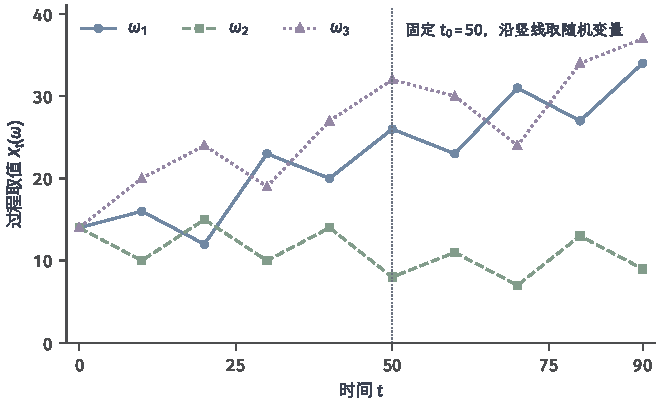
\includegraphics[width=\linewidth]{figures/02-mathematical-preliminaries-lower/01-random-variables-distributions-and-causality/matplotlib/rv-paths/figure.pdf}
  \caption{同一过程的路径与时刻截面是不同对象。图为人为给定的三条示意路径，竖虚线固定时刻\(t_0\)；交点展示该时刻可能出现的不同值，并非用三条路径估计出的概率密度。}
\label{fig:rv-paths}
\end{figure}

若对每个固定\(t\)，\(\mathbb P(X_t=Y_t)=1\)，称\(X,Y\)互为版本；若
\(\mathbb P(\forall t,\ X_t=Y_t)=1\)，则称不可区分。不可数时间集上，两者不同。
例如\(U\)在\([0,1]\)均匀分布，\(X_t=\mathbb I_{\{t=U\}}\)、\(Y_t=0\)：
每个固定时刻两者几乎必然相等，但每条\(X\)路径都在某个时刻出现尖点。
若两个版本都具有右连续路径，则先在可数稠密时刻同时相等，再用右连续性推广，才得到不可区分。

描述连续路径的粗糙程度时，称\(x\)在紧时间区间上具有正指数\(\alpha\)的Hölder连续性，是指存在有限\(C_x\)，使
\[
 |x(t)-x(s)|\leq C_x|t-s|^\alpha
 \quad\text{对区间内所有 }s,t\text{成立}.
\]
随机路径允许常数\(C_x\)依赖具体实现。\(\alpha=1\)就是Lipschitz条件；在短时间差上，较小的正指数给出较弱的约束。例如\(\sqrt t\)满足
\(|\sqrt t-\sqrt s|\leq|t-s|^{1/2}\)，却在零点附近不满足Lipschitz条件。这里是路径正则性，与同名的Hölder积分不等式不同。

得到连续版本的一项常用充分条件是Kolmogorov连续性准则：若在紧时间区间上存在
\(p>0,\beta>0,C<\infty\)，使
\[
\mathbb E|X_t-X_s|^p\leq C|t-s|^{1+\beta},
\]
则存在连续版本，并可取得任意小于\(\beta/p\)的正Hölder指数；该条件本身不保证达到端点\(\beta/p\)。条件控制的是整族短时增量，不能由每个时刻分布连续推出。对Brownian增量，四阶矩为\(3|t-s|^2\)，足以给出连续版本；更高阶矩可把Hölder指数推进到任意小于\(1/2\)。

\subsection{随机误差的收敛与量级}
\label{sec:stoch-convergence-criteria}
重复测量时，一个自然的问题是：样本均值的误差是否会随样本数增多而缩小。要严格表述“缩小”，先要说明控制的是哪个量：大偏差发生的概率、整条样本路径，还是平均平方误差。下面先约定这几种收敛判据，后文在具体估计问题中使用它们，并在第~\ref{sec:rv-sequence-process-convergence}节证明彼此的关系。
\paragraph{随机结果的收敛判据}
\begin{definition}[随机变量的收敛]
  \label{def:probability-random-convergence}
以下依概率、几乎必然和\(L^p\)收敛要求\(X_n,X\)定义在同一概率空间上；依分布收敛只要求它们的分布有定义。若对每个\(\varepsilon>0\)，
\[ \mathbb{P}(|X_n-X|>\varepsilon)\to0, \]
就称\(X_n\)依概率收敛到\(X\)，记作\(X_n\to_{\mathbb{P}}X\)。它允许小概率坏事件随\(n\)改变，只要求每个固定容差外的概率趋于零。

若
\[ \mathbb{P}\left(
    \lim_{n\to\infty}X_n=X\right)=1, \]
就称\(X_n\)几乎必然收敛到\(X\)，记作\(X_n\to_{\mathrm{a.s.}}X\)。它要求除一个
固定零测集外，每条样本路径最终都收敛，因而比依概率收敛更强。

对\(1\leq p<\infty\)，若\(X_n,X\in L^p(\mathbb P)\)且\(\mathbb{E}[|X_n-X|^p]\to0\)，就称\(X_n\)在\(L^p\)中收敛。特别地，\(p=2\)称为均方收敛。

若对\(X\)的每个分布函数连续点\(x\)，都有
\[ F_{X_n}(x)\to F_X(x), \]
就称\(X_n\)依分布收敛到\(X\)，记作\(X_n\Rightarrow X\)。它只比较边缘分布，不要求变量定义在同一概率空间上。

\end{definition}

\paragraph{随机误差的概率阶}
渐近分析还要比较随机误差与某个确定尺度的相对大小，例如判断余项相对于主项是否可以忽略。下面的概率阶记号把这种比较写成可以直接检验的概率条件。
\begin{definition}[概率阶记号]
  \label{def:statistics-probability-order}
\term{概率有界}（bounded in probability）把“随机量不会随\(n\)逃向无穷”写成
可检验的概率条件。若对每个\(\epsilon>0\)，都存在有限常数\(M\)和整数\(n_0\)，使
\[
  \sup_{n\geq n_0}\mathbb{P}(|X_n|>M)<\epsilon,
\]
就记\(X_n=O_{\mathbb{P}}(1)\)。若\(X_n\to_{\mathbb{P}}0\)，则记
\(X_n=o_{\mathbb{P}}(1)\)。对确定正数列\(a_n\)，约定\(X_n=O_{\mathbb P}(a_n)\)与\(X_n=o_{\mathbb P}(a_n)\)分别表示\(X_n/a_n=O_{\mathbb P}(1)\)与\(X_n/a_n=o_{\mathbb P}(1)\)。
\end{definition}

\section{随机序列与过程的依赖关系}
\label{sec:stoch-process-dependence}
一组读数可以共享同一背景，也可以随状态逐步演化。要判断重排记录、压缩历史或平移时间会保留哪些概率结论，需要分别规定联合规律的对称性、下一状态的条件规律、下一读数的条件均值与时间平移的规律。这些条件可以同时成立，不能互相替代。

\subsection{序列重排下的交换关系}

若一批观测没有需要保留的顺序，可以检查重排记录以后联合规律是否改变。这一对称要求只比较重排前后的规律，不要求各项独立；共享同一背景的观测也可能满足它。
\label{sec:rv-exchangeability}
% Baseline P:2279-2289
\begin{definition}[可交换随机变量]
  \label{def:probability-exchangeability}
随机变量\(Z_1,\ldots,Z_m\)若对每个排列\(\pi\)都有
\[ (Z_1,\ldots,Z_m)
  \overset{\mathrm{d}}{=}(Z_{\pi(1)},\ldots,Z_{\pi(m)}), \]
就称它们\term{可交换}（exchangeable）。
\end{definition}
独立同分布蕴含可交换，但反向不成立。
例如先抽取取值于\([0,1]\)的非退化随机概率\(\Theta\)，再条件于\(\Theta\)独立生成Bernoulli观测；边缘上这些观测可交换，却因共享\(\Theta\)而相关。

可交换性不提供样本平均的独立乘积结构，因而不能直接代入Hoeffding证明。
它提供的是标签位置的对称性：若评分规则在重排观测时只把分数作同样的重排，
并且分数几乎必然没有并列，则每个分数占据每个秩的概率都是\(1/m\)。
因为所有标签机会相同，而每个秩又恰由一个标签占据，概率总和必须为\(1\)。
有并列时，可为每个分数附加一个服从\(\operatorname{Unif}(0,1)\)的随机数，
这些随机数相互独立，并且独立于全部分数。
把分数按大小排序，分数相同时再按附加的随机数排序；这样既保留对称性，又消除并列，从而恢复均匀的秩。
若采用不随机化的并列规则，则通常只能得到相应的保守概率界。
后面的共形预测会明确区分这两种处理，使用它们各自的有限样本结论。
例如共享参数\(\Theta\sim\operatorname{Beta}(2,2)\)，给定\(\Theta\)后
\(X_i\)独立服从\(\operatorname{Bernoulli}(\Theta)\)。每个边缘的成功率为\(1/2\)，但对\(i\ne j\)，塔式性质给出
\[
\operatorname{Cov}(X_i,X_j)
=\mathbb E[\Theta^2]-(\mathbb E\Theta)^2
=\operatorname{Var}(\Theta)=\frac1{20}.
\]
因此\(\mathbb P(X_1=X_2=1)=0.3\)，大于独立情况下的\(0.25\)。
共享背景使一串成功更常一起出现，却没有偏爱某个观测编号。有限可交换性本身不保证一定存在这样的独立混合表示；本例是可交换依赖的一种构造。

\subsection{历史条件下的状态依赖}

预测下一时刻时，完整历史通常含有很多记录。若当前状态已经概括其中与下一步有关的信息，给定当前状态后继续加入旧记录就不应改变下一步条件分布。Markov关系将这个建模要求写成条件分布的等式。
\label{sec:rv-markov}
\label{sec:stoch-martingales-stopping-sequential-concentration}
先约定时刻\(t\)已知哪些记录。滤过使“完整历史”成为可用于条件期望的数学对象；适应性检查当前状态是否已经可知，可预测性则检查下一步所用系数是否在新噪声揭晓前确定。
% Baseline S:371-384
\begin{definition}[滤过、适应与可预测性]
  \label{def:stoch-filtration-adaptation-predictability}
在概率空间
$(\Omega,\mathcal{F},\mathbb{P})$上，令每个$\mathcal{F}_t$都是
$\mathcal{F}$的子$\sigma$代数，并且
\[
  \mathcal{F}_0\subseteq\mathcal{F}_1\subseteq\cdots\subseteq\mathcal{F}.
\]
这列递增的子$\sigma$代数称为\term{滤过}（filtration），可以理解为随时间增长的信息。
随机变量$X_t$若对
$\mathcal{F}_t$可测，就称它在时刻$t$已经可知；若每个$t$都如此，称$(X_t)$适应于该滤过。对$t\geq1$，过程$(H_t)$若$H_t$对
$\mathcal{F}_{t-1}$可测，就称为\term{可预测过程}（predictable process）。
\end{definition}
这里的“可预测”不是说$H_t$没有随机性，而是说它可以由第$t$次新噪声到来之前的信息确定。
% Baseline S:441-447
逐步观测还可能在读数首次越过阈值时结束，结束轮次因此是随机的。可实施的停止规则必须只用已经取得的记录：到当前轮次就能判断是否已经结束。下面的条件排除依赖未来记录的停止选择。
\begin{definition}[停时]
  \label{def:stoch-stopping-time}
  相对于滤过\((\mathcal F_t)_{t\geq0}\)，取值于\(\mathbb N_0\cup\{\infty\}\)的随机时刻$\tau$若满足$\{\tau\leq t\}\in\mathcal{F}_t$对每个整数$t\geq0$成立，就称为\term{停时}（stopping time）。
\end{definition}
到时刻$t$为止已有的信息足以判断是否已经停止；“最后一次
达到最大值的时刻”通常需要看到未来，不一定是停时。

% Baseline S:69-131
\begin{definition}[Markov链]
  \label{def:stoch-markov-chain}
设$(Z_t)_{t\geq0}$取值于可测空间$(\mathcal{Z},\mathcal{A})$。若对每个
$B\in\mathcal{A}$，
\[
  \mathbb{P}(Z_{t+1}\in B\mid Z_0,\ldots,Z_t)
  =
  \mathbb{P}(Z_{t+1}\in B\mid Z_t),
\]
则称$(Z_t)$为\term{Markov链}（Markov chain）；上述条件等式按几乎必然意义理解。
\end{definition}
这个条件不是说过去没有影响，而是
说当前状态已经保存了预测下一步所需的全部历史信息。
即使当前状态足以预测下一步，同一个状态在上午和晚上也可能使用不同的转移规律。若进一步假设规律不随轮次改变，就可以反复使用同一个核，并用核的复合计算多步分布。
\begin{definition}[时间齐次Markov链]
  \label{def:stoch-time-homogeneous-chain}
  若存在从\((\mathcal Z,\mathcal A)\)到自身的概率核\(P\)，使所有\(t\geq0\)、\(B\in\mathcal A\)都满足
  \[ \mathbb P(Z_{t+1}\in B\mid Z_t)=P(Z_t,B)\quad\text{几乎必然}, \]
  则该Markov链称为\term{时间齐次的}（time-homogeneous）。
\end{definition}
时间齐次描述机制不变，不代表$Z_t$的边缘分布不随时间改变\scite{math-meyn2009markov}。

概率核的两项要求见定义~\ref{def:probability-kernel}：每个状态对应合法的下一步分布，而每个事件的概率随当前状态可测地变化。对有界可测函数$f$，记
\[
  Pf(z)=\int_{\mathcal{Z}}f(z')P(z,\mathrm{d}z').
\]
两个核的复合按
\[
  (PQ)(z,B)
  =
  \int_{\mathcal{Z}}Q(z',B)P(z,\mathrm{d}z')
\]
定义；它表示先按$P$走一步，再按$Q$走一步。令$P^0(z,B)=\mathbb{I}\{z\in B\}$，
$P^{m+1}=P^mP$，则时间齐次链满足
\begin{equation}
  \mathbb{P}(Z_{t+m}\in B\mid Z_t=z)=P^m(z,B),
  \qquad
  P^{m+n}(z,B)
  =
  \int_{\mathcal{Z}}P^n(z',B)P^m(z,\mathrm{d}z').
  \label{eq:stoch-chapman-kolmogorov}
\end{equation}
第一个等式作为条件分布恒等式只要求对\(Z_t\)的分布几乎处处成立；不可达状态上的条件版本并不由观测规律确定。核的复合则在每个\(z\)上有定义。第二个等式称为\term{Chapman--Kolmogorov关系}。证明可直接使用条件概率的塔式性质：
给定$Z_{t+m}=z'$后，Markov性质把后$n$步的条件概率化为$P^n(z',B)$；再对
$Z_{t+m}$在给定$Z_t=z$时的分布$P^m(z,\mathrm{d}z')$积分，就得到右侧。取$n=1$
并归纳，还同时证明了第一个等式及核幂确实给出多步转移。

核给出了分布怎样前进一步。现在反过来寻找一种初始分布，使前进一步后各事件的概率都保持不变：对旧状态分布混合下一步核，得到的仍是原分布。这样的分布是分布更新的不动点，而不是要求单个状态停止移动。
\begin{definition}[平稳分布]
  \label{def:stoch-stationary-distribution}
概率分布$\pi$若满足
\begin{equation}
  \pi(B)=\int_{\mathcal{Z}}P(z,B)\,\pi(\mathrm{d}z),
  \qquad B\in\mathcal{A},
  \label{eq:stoch-stationary-distribution}
\end{equation}
就称为$P$的\term{平稳分布}（stationary distribution）。
\end{definition}
若$Z_0\sim\pi$，式
\eqref{eq:stoch-stationary-distribution}保证每个$Z_t$仍服从$\pi$；若从指定状态
$z_0$启动，平稳性本身却没有说明$\mathcal{L}(Z_t)$会趋向$\pi$。恒等转移核
$P(z,B)=\mathbb{I}\{z\in B\}$保持任意分布，但它永远不忘记初态，这已经表明“保持
目标”和“到达目标”是两项不同要求。

% Baseline S:151-163
要验证一张候选分布被转移核保持，可以直接核对上面的积分等式，也可以寻找更容易逐对核验的充分条件。在有限状态下，若每对状态之间的正向流量\(\pi_iP_{i,j}\)都等于反向流量\(\pi_jP_{j,i}\)，对所有来源求和就能保证各处总质量不变。下面把这一逐对流量条件推广到一般状态空间。
\begin{definition}[细致平衡]
  \label{def:stoch-detailed-balance}
概率核\(P\)与概率测度\(\pi\)满足\term{细致平衡}（detailed balance），若以下两个联合测度在\(\mathcal Z\times\mathcal Z\)上相同：
\begin{equation}
  \pi(\mathrm{d}z)P(z,\mathrm{d}z')
  =\pi(\mathrm{d}z')P(z',\mathrm{d}z).
  \label{eq:stoch-detailed-balance}
\end{equation}
\end{definition}
它要求平稳运行时任意两处之间的概率流量正反相等。对$z$积分便得到
\eqref{eq:stoch-stationary-distribution}，所以细致平衡足以推出平稳性。反向不成立：
围绕三个状态单向循环的链可以保持均匀分布，却没有逐边对称的反向流。细致平衡是构造
采样链的便利证书，不是遍历平均成立的必要定义。

\subsection{历史条件下的均值关系}

完整条件分布不变是一项强要求。有时只知道新增量在已有历史下没有平均漂移，方差和其他形状仍可随历史改变。把这类增量累计起来，得到条件均值保持当前值的过程，称为鞅；下面用可积性使这个均值等式有意义。
\label{sec:rv-martingales}
% Baseline S:386-425
\begin{definition}[鞅与鞅差]
  \label{def:stoch-martingale}
可积过程$(M_t)$若适应于$(\mathcal{F}_t)$，并对每个整数$t\geq1$满足
\begin{equation}
  \mathbb{E}[M_t\mid\mathcal{F}_{t-1}]=M_{t-1},
  \label{eq:stoch-martingale-definition}
\end{equation}
就称为\term{鞅}（martingale）。增量$X_t=M_t-M_{t-1}$满足
\begin{equation}
  \mathbb{E}[X_t\mid\mathcal{F}_{t-1}]=0,
  \label{eq:stoch-martingale-difference}
\end{equation}
称为\term{鞅差}（martingale difference）。若条件等式改为\(\mathbb E[M_t\mid\mathcal F_{t-1}]\leq M_{t-1}\)，称\((M_t)\)为超鞅；改为\(\geq\)时称为次鞅。两者也要求每个时刻可积且适应。
\end{definition}
这里的\(t\)是离散整数时刻。连续时间的定义把相邻时刻条件换成：
对任意\(0\leq s\leq t\)，
\(\mathbb E[M_t\mid\mathcal F_s]=M_s\)几乎必然；每个时刻仍须可积且适应。
超鞅与次鞅分别改用\(\leq\)和\(\geq\)。后面的补偿计数与布朗运动均使用这一连续时间版本。
无条件零均值不够：若$X_t$可以由过去
预测，累计和仍可能形成系统漂移；式~\eqref{eq:stoch-martingale-difference}排除的正是
这种可利用的条件平均。

\begin{example}[公平随机游走与按过去下注]
  \label{ex:stoch-predictable-betting}
  设$\varepsilon_t$独立取$\{-1,1\}$，两种取值概率均为$1/2$，并令
  $\mathcal{F}_t=\sigma(\varepsilon_1,\ldots,\varepsilon_t)$。公平随机游走
  $S_t=\sum_{s=1}^{t}\varepsilon_s$是鞅。

  现在允许下注额$H_t$根据过去结果选择，只要求$H_t$对
  $\mathcal{F}_{t-1}$可测，并使$H_t\varepsilon_t$可积。另设\(M_0\)可积且对\(\mathcal F_0\)可测。财富过程
  \[
    M_t=M_0+\sum_{s=1}^{t}H_s\varepsilon_s
  \]
  仍是鞅，因为
  \[
    \mathbb{E}[H_t\varepsilon_t\mid\mathcal{F}_{t-1}]
    =
    H_t\mathbb{E}[\varepsilon_t\mid\mathcal{F}_{t-1}]
    =0.
  \]
  策略可以追涨、反向或在某些历史后停止下注，但只要它不能偷看$\varepsilon_t$，就不能
  改变下一笔收益的条件均值。若$H_t$依赖当前尚未揭晓的$\varepsilon_t$，上面的等式便
  失去依据。
\end{example}
条件均值保持本身没有规定长期极限。定理~\ref{thm:rv-l2-martingale-convergence}将在序列收敛中补充二阶矩有界条件，说明累计误差何时具有路径极限与均方极限。

这里值得先分清两个常被混淆的说法。例~\ref{ex:stoch-predictable-betting}说明“每期条件均值为零”不等于“不能亏损”：公平下注策略的财富可以使已实现路径长期为负，只是这种路径不能用已知历史提前识别。可预测性要求下注额在新噪声揭晓前已经由历史确定；收益增量的零条件均值还需要噪声在该历史下均值为零。两项条件共同支持上面的鞅结论，都不保证单条实现不亏损。相应地，鞅差的零条件均值也不推出增量之间的无条件独立性：增量可以有相同的方差、可以有依赖的绝对值，甚至方差本身随历史变化（例如每期下注额随财富调整），但只要给定历史后条件均值为零，累计和仍是鞅。把鞅差一律当作独立同分布变量，会漏掉允许历史依赖和条件异方差的情形。

第二个区分关乎定义中条件\(\sigma\)代数的选择。条件期望\(\mathbb E[M_t\mid\mathcal F_{t-1}]\)随\(\mathcal F_{t-1}\)变化：信息更多时，条件均值可能不再等于\(M_{t-1}\)。因此同一序列在较粗的信息流下可能是鞅，在较细的信息流下则不是。例如令独立符号\(\varepsilon_t\)等概率取\(\pm1\)，\(M_t=\sum_{s=1}^t\varepsilon_s\)，自然历史为\(\mathcal F_t=\sigma(\varepsilon_1,\ldots,\varepsilon_t)\)。给定\(\mathcal F_{t-1}\)后，下一增量仍均值为零，所以\(M_t\)是鞅。若扩大信息流为\(\mathcal G_t=\sigma(\varepsilon_1,\ldots,\varepsilon_{t+1})\)，则\(M_t\)仍适应，但\(\mathcal G_{t-1}\)已经揭晓\(\varepsilon_t\)，于是\(\mathbb E[M_t\mid\mathcal G_{t-1}]=M_t\)，通常不等于\(M_{t-1}\)。因此独立零均值增量只保证相对于不预先揭晓这些增量的适当历史是鞅，不能保证相对于任意扩大的信息流仍是鞅。使用鞅结论时必须说明信息流是什么，这与条件期望的定义要求一致。

\subsection{时间平移下的分布关系}
\label{sec:rv-stationarity}
% Baseline S:132-149
把观测窗口从今天移到明天后，若整组读数的联合规律保持不变，就可以用时间平移来表达这种稳定的统计结构。这里比较的是窗口中的联合分布；仅保持单时刻的边缘分布，还不足以确定两次读数之间的联系。
\begin{definition}[平稳过程]
  \label{def:stoch-stationary-process}
  离散时间过程\((Z_t)_{t\geq0}\)称为\term{平稳过程}（stationary process），若任意正整数\(m\)、时刻\(t_1,\ldots,t_m\geq0\)及整数\(h\geq0\)都满足
  \[ (Z_{t_1},\ldots,Z_{t_m})\overset{\mathrm d}{=}(Z_{t_1+h},\ldots,Z_{t_m+h}). \]
\end{definition}
对时间齐次Markov链，若$Z_0\sim\pi$且
$\pi P=\pi$，则
\[
  \mathbb{P}(Z_0\in\mathrm{d}z_0,\ldots,Z_m\in\mathrm{d}z_m)
  =
  \pi(\mathrm{d}z_0)
  \prod_{j=1}^{m}P(z_{j-1},\mathrm{d}z_j).
\]
把起点向后平移一格时，先对$z_0$积分，$\pi P=\pi$把$Z_1$的边缘重新化为$\pi$，
其余转移核不变；反复应用便证明所有有限维分布都不随平移改变。因此，从平稳分布启动的
时间齐次链是平稳过程。只知道某一个时刻的边缘分布等于$\pi$，却没有核不变或联合分布
条件时，不能据此断言整个过程平稳。
完整联合分布的平移不变性较强。若当前只计算平均值和二阶误差，可以先保留较少的要求：各时刻均值不变，两次读数的协方差只由相隔多久决定。这个较弱条件足以组织二阶计算，却未必保留全部分布形状。
\begin{definition}[二阶平稳]
\label{def:rv-second-order-stationary}
实值过程二阶矩有限，若均值与时间无关，且
\(\operatorname{Cov}(X_s,X_t)\)只依赖时间差\(t-s\)，称为\term{二阶平稳}（second-order stationarity），也称弱平稳。
\end{definition}
严格平稳加有限二阶矩推出二阶平稳；反向一般不成立。例如相互独立的序列在偶数时刻取标准高斯分布，在奇数时刻等概率取\(\pm1\)。均值均为零，方差均为一，非同时刻协方差均为零，所以二阶平稳，但一维边缘随奇偶变化，并不严格平稳。联合高斯过程则由均值与协方差完全决定有限维规律，因此此时二阶平稳足以推出严格平稳。
Brownian运动和零均值随机游走可以是Markov鞅，但方差随时间增长，不是平稳过程；其增量却可平稳。核的不变分布、从任意初态趋向它，以及过程已经从该分布启动，仍是三项不同命题。

\section{随机序列与过程的生成}
\label{sec:stoch-sequence-process-generation}
依赖条件约束一族已有变量的联合规律；构造模型还要给出能够产生这些联合规律的规则。累计独立增量、反复应用转移核、记录事件到达以及指定高斯协方差，分别形成不同的生成方式。有限分割上的相容概率向量还可让整张概率测度成为随机对象。

\subsection{基于状态转移的随机序列生成}
\label{sec:rv-state-generation}

给定当前状态后抽取一步增量，再重复这一操作，可以生成整条随机序列。随机游走用增量相加确定下一位置；一般Markov链则直接用转移核给出下一状态的条件分布。它们都保留逐步生成的次序，相邻位置之间通常相关。

\subsubsection{基于增量累计的随机游走生成}
\label{sec:rv-random-walk}
给定独立同分布增量\(\xi_i\)，定义
\(S_0=0\)、\(S_n=\sum_{i=1}^n\xi_i\)，称为\term{随机游走}（random walk）。若
\(\mathbb E\xi_i=\mu\)、\(\operatorname{Var}(\xi_i)=\sigma^2<\infty\)，则
\[
\mathbb ES_n=n\mu,\qquad
\operatorname{Var}(S_n)=n\sigma^2,\qquad
\operatorname{Cov}(S_m,S_n)=\min(m,n)\sigma^2.
\]
当\(\sigma^2>0\)且\(m,n\geq1\)时，位置之间的协方差为正，所以不能把不同位置当作独立观测。
\(S_n-n\mu\)相对于增量的自然滤过是鞅，\(S_n\)本身还具有Markov性。
若\(\mathbb P(\xi_i=1)=p\)、\(\mathbb P(\xi_i=-1)=1-p\)，则漂移为
\(2p-1\)、单步方差为\(4p(1-p)\)。取\(p=0.6\)，十步均值为\(2\)、方差为\(9.6\)；某一条十步路径却不必靠近均值。
大数定律控制\(S_n/n\)，当\(\sigma>0\)时，中心极限定理控制
\((S_n-n\mu)/(\sigma\sqrt n)\)；整个折线在缩放下的极限则使用第~\ref{sec:rv-path-convergence}节的路径定理。

\subsubsection{基于转移核的Markov链生成}
Markov核给出一步条件规律：从当前状态出发，下一步可能到哪些状态、各以什么概率。但只凭这一步还不够，还要回答三个问题：多步以后状态如何分布，边缘分布能否趋向某个极限，长期平均又由什么决定。下面分别需要核复合及返回条件。

\paragraph{状态转移与多步分布}
% Baseline S:165-185
\begin{example}[相关的两状态观测]
  \label{ex:stoch-two-state-chain}
  令$Z_t\in\{0,2\}$，并把观测直接取为$Y_t=Z_t$。转移矩阵按状态$0,2$排序为
  \[
    \bm{P}
    =
    \begin{pmatrix}
      0.9 & 0.1\\
      0.2 & 0.8
    \end{pmatrix}.
  \]
  平稳分布为$\bm{\pi}=(2/3,1/3)^\top$，因为
  $\bm{P}^{\top}\bm{\pi}=\bm{\pi}$。在这项平稳分布下，单次观测的均值是
  \[
    \mu=\mathbb{E}_{\pi}[Y]=\frac23.
  \]
  两条跨状态概率流都等于
  $(2/3)\times0.1=(1/3)\times0.2=1/15$，故该链还满足细致平衡。
  从状态$0$启动时，$Y_0$不服从$\pi$；转移规则时间齐次，过程却要经过一段时间才
  接近平稳。
\end{example}
% Baseline S:189-197
这个例子能在两个状态之间来回移动，且允许原地停留。要判断一般链能否忘记初态，需要把这两项作用分开：是否任意状态都能经若干步到达另一个状态，以及返回是否只能发生在某些固定倍数的步数上。不可约性检查前者，周期检查后者。
\begin{definition}[有限链的不可约性与周期]
  \label{def:stoch-finite-irreducibility-period}
  有限状态Markov链满足\term{不可约性}（irreducibility），若对任意状态\(i,j\)存在整数\(m\geq0\)，使\(P^m(i,\{j\})>0\)。若返回步数集合非空，状态\(i\)的\term{周期}（period）定义为
  \[ d_i=\gcd\{m\geq1:P^m(i,\{i\})>0\}. \]
  不可约链的全部状态具有共同周期；该周期为\(1\)时，称链为\term{非周期的}（aperiodic）。
\end{definition}
把相互可达的状态归在一起，得到互达等价类；若从一个类内出发，一步转移不会离开该类，就称它封闭。
不可约性要求所有状态属于同一个互达类，并在有限状态下保证平稳分布唯一。

在前面的两状态例子中，令\(q_t=\mathbb P(Y_t=2)\)。一步转移给出
\[
q_{t+1}=0.1(1-q_t)+0.8q_t=0.1+0.7q_t,
\qquad q_t=\frac13+0.7^t\left(q_0-\frac13\right).
\]
从\(q_0=0\)出发，前两步为\(q_1=0.1,q_2=0.17\)，而不是立即得到
\(1/3\)。不变分布给出递推的不动点；这里的收敛则由偏差系数\(0.7\)另行证明。

\subsection{基于到达计数的随机过程生成}
\label{sec:rv-poisson}
事件到达使状态按次跳变。固定窗口内的计数可以服从Poisson分布，但只有规定不同窗口间的联合关系，才能得到Poisson过程。

\paragraph{事件计数与短时跳跃}
\begin{definition}[齐次Poisson过程]
\label{def:rv-poisson-process}
给定速率\(\lambda>0\)和滤过\((\mathcal F_t)_{t\geq0}\)，计数过程
\((N_t)_{t\geq0}\)称为相对于该滤过的齐次\term{泊松过程}（Poisson process），若它适应于滤过，
\(N_0=0\)几乎必然，路径几乎必然右连续、非减、取非负整数且每次跳跃为一，并满足
\[
N_t-N_s\ \perp\ \mathcal F_s,\qquad
N_t-N_s\sim\operatorname{Poisson}(\lambda(t-s)),
\quad 0\leq s<t.
\]
\end{definition}
这里的平稳性属于增量，而非\(N_t\)本身：计数均值随时间线性增长。
对互不相交、按时间排列的区间，逐步使用独立于过去的条件，便得到增量相互独立。
相对于自然滤过给出过程后，不能随意加入未来信息而仍称其增量独立于历史。

短区间\(h\downarrow0\)内，
\[
\begin{aligned}
\mathbb P(N_{t+h}-N_t=0)&=1-\lambda h+O(h^2),\\
\mathbb P(N_{t+h}-N_t=1)&=\lambda h+O(h^2),\\
\mathbb P(N_{t+h}-N_t\geq2)&=O(h^2).
\end{aligned}
\]
一次跳跃的\emph{概率}是一阶小量，发生跳跃时的\emph{幅度}却始终为一。
令\(T_k=\inf\{t:N_t\geq k\}\)为第\(k\)次到达时刻。有限\(t\)内
\(N_t<\infty\)几乎必然，因而只有有限次跳跃；这是有限活动过程。
左极限\(N_{t-}=\lim_{s\uparrow t}N_s\)记录跳跃发生前的计数，跳跃量记为
\(\Delta N_t=N_t-N_{t-}\)。

Poisson计数与指数等待是同一齐次到达机制的两个侧面。首次到达时间满足
\[
% Baseline P:914-923
  \mathbb{P}(T_1>t)
  =
  \mathbb{P}(N_t=0)
  =
  e^{-\lambda t}.
\]
所以\(T_1\)服从速率为\(\lambda\)的指数分布；独立平稳增量进一步使相邻到达间隔独立
同分布。反过来，用独立同分布的指数等待时间累加生成到达时刻，所得计数过程的
\(N_t\)服从\(\operatorname{Poisson}(\lambda t)\)。这里的联系依赖齐次性和独立增量，
不能由两个边缘分布的名称单独推出。
更具体地，独立增量的短区间概率给出前\(k\)个到达时刻在
\(0<t_1<\cdots<t_k\)上的联合密度
\(\lambda^k e^{-\lambda t_k}\)。换成等待间隔
\(E_i=T_i-T_{i-1}\)，其中\(T_0=0\)，Jacobian为一，密度变成
\(\prod_i\lambda e^{-\lambda e_i}\)，证明间隔独立且均为指数分布。
等待\(k\)次到达的总时长因此是
\(\operatorname{Gamma}(k,\lambda)\)，采用前面约定的速率参数。
反向从独立指数间隔构造时，
\(\mathbb P(T_k\leq t<T_{k+1})=e^{-\lambda t}(\lambda t)^k/k!\)；
无记忆性保证每个确定时刻之后的剩余等待仍指数，从而得到独立平稳增量。

若每次到达还带来随机量\(J_k\)，其中\(J_k\)独立同分布且独立于计数过程，则
\[
C_t=\sum_{k=1}^{N_t}J_k
\]
称为\term{复合泊松过程}（compound Poisson process）。其跳跃量不必为一，也可为负；给定\(N_t\)以后再求条件均值和全方差，可得
\[
\mathbb EC_t=\lambda t\,\mathbb EJ_1,\qquad
\operatorname{Var}(C_t)=\lambda t\,\mathbb EJ_1^2
\]
（第一式需一阶绝对矩有限，第二式需二阶矩有限）。第二式不是
\(\lambda t\operatorname{Var}(J_1)\)，因为事件数本身也随机。
这里的Poisson过程描述事件到达；定义~\ref{def:stoch-markov-poisson-equation}中的Poisson方程描述Markov核下的均值校正，它们不是同一个对象。

\paragraph{非恒定强度下的首次到达}
恒定速率假设意味着相同长度的窗口具有相同的平均到达数。若事件密度随时间或沿射线的位置改变，就需要用一个确定的强度函数\(\lambda(t)\geq0\)描述局部到达率。假定它在每个有界区间上可积，并定义累计强度
\[
 \Lambda(t)=\int_0^t\lambda(u)\,\mathrm du.
\]
取单位速率的齐次Poisson过程\(M\)，令\(N_t=M_{\Lambda(t)}\)，便得到一个非齐次泊松过程（nonhomogeneous Poisson process）。它具有独立增量，且
\[
 N_t-N_s\sim\operatorname{Poisson}\bigl(\Lambda(t)-\Lambda(s)\bigr),
 \qquad 0\leq s<t.
\]
局部可积性使每个有限区间内的累计强度有限，从而排除有限时间内无穷次到达。时间变换改变了不同区间的平均到达数；除非\(\lambda\)几乎处处为常数，增量一般不再平稳。

首次到达\(T_1=\inf\{t:N_t\geq1\}\)晚于\(t\)，等价于此前计数为零。因此其生存概率和有限时刻的密度分别为
\begin{equation}
 \mathbb P(T_1>t)=e^{-\Lambda(t)},\qquad
 f_{T_1}(t)=\lambda(t)e^{-\Lambda(t)}
 \quad\text{几乎处处},
 \label{eq:stoch-nonhomogeneous-first-arrival}
\end{equation}
第二式由第一式对\(t\)求导得到，使用了\(\Lambda\)的绝对连续性。若\(\Lambda(\infty)<\infty\)，则
\(\mathbb P(T_1=\infty)=e^{-\Lambda(\infty)}>0\)；这部分质量表示永不到达，有限时刻的密度积分因而可以小于一。

给定直到\(s\)仍未到达，再等待\(u\)的概率为
\[
 \mathbb P(T_1>s+u\mid T_1>s)
 =\exp\left\{-\int_s^{s+u}\lambda(v)\,\mathrm dv\right\}.
\]
它通常依赖开始等待的位置\(s\)，所以到达间隔不能继续当作同分布的指数变量。例如\(\lambda(t)=\beta t\)、\(\beta>0\)时，生存概率为\(e^{-\beta t^2/2}\)，并非指数分布的生存函数。若将\(t\)解释为射线路程，同一无事件概率给出指数透射形式，而\(\lambda(t)e^{-\Lambda(t)}\)给出首次相互作用的位置密度；这只是同一个计数模型的取值解释，离散渲染积分另行处理\scite{math-kallenberg2021probability}。

\paragraph{平均到达与补偿增量}
先回到恒定速率\(\lambda\)的齐次计数，每段长度为\(h\)的时间平均增加\(\lambda h\)。从原计数中减去这一可预测平均趋势，得到\term{补偿泊松过程}（compensated Poisson process）
\[
\widetilde N_t=N_t-\lambda t.
\]
\begin{theorem}[Poisson补偿的鞅性质]
\label{thm:rv-compensated-poisson}
相对于定义~\ref{def:rv-poisson-process}中的滤过，
\(\widetilde N_t\)是平方可积鞅，且
\[
\mathbb E[(\widetilde N_t-\widetilde N_s)^2\mid\mathcal F_s]
=\lambda(t-s),\qquad
\widetilde N_t^2-\lambda t\text{也是鞅}.
\]
\end{theorem}
\begin{proof}
独立增量使给定\(\mathcal F_s\)后的计数增量仍有均值及方差
\(\lambda(t-s)\)。减去均值后，条件均值为零，条件二阶矩就是该方差。
再展开
\(\widetilde N_t^2=(\widetilde N_s+
(\widetilde N_t-\widetilde N_s))^2\)，交叉项条件期望为零，剩余新增二阶矩为
\(\lambda(t-s)\)，得到最后一个鞅结论。
\end{proof}
补偿并未抹平跳跃。图~\ref{fig:rv-poisson-compensation}中，计数在到达之间保持不变，补偿路径则以斜率\(-\lambda\)下降；每个到达时刻仍向上跳一。
\begin{figure}[htbp]
  \centering
  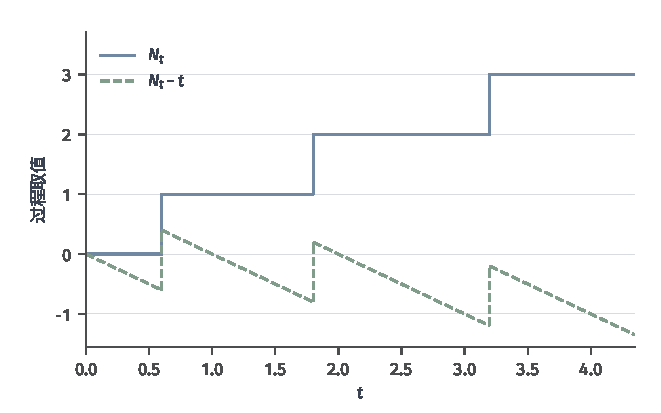
\includegraphics[width=\linewidth]{figures/02-mathematical-preliminaries-lower/01-random-variables-distributions-and-causality/matplotlib/rv-poisson-compensation/figure.pdf}
  \caption{给定三次到达时刻的教学路径，取\(\lambda=1\)。蓝线为计数\(N_t\)，绿虚线为\(\widetilde N_t=N_t-t\)；两条路径在同一时刻跳跃且跳跃量相同。减去的是平均趋势，不是实现中的跳跃。}
\label{fig:rv-poisson-compensation}
\end{figure}
平方跳跃累计为
\(\sum_{s\leq t}(\Delta\widetilde N_s)^2=N_t\)，是随机量；
其可预测平均累计为\(\lambda t\)，不是同一个量。在有限活动区间上，细分路径的平方增量和趋向跳跃平方和，连续线性漂移贡献趋零，故可记
\[
[\widetilde N]_t=N_t,\qquad
\langle\widetilde N\rangle_t=\lambda t.
\]
后一个量是使\(\widetilde N_t^2-\langle\widetilde N\rangle_t\)成为鞅的可预测补偿。离散历史相关偏差中的相应定义见定义~\ref{def:stoch-predictable-quadratic-variation}。对确定分割，这个有限活动情形的路径计算可逐条进行；连续粗糙路径的二次变差将在下一例说明。

复合情形若\(\mathbb E|J_1|<\infty\)，则
\(C_t-\lambda t\,\mathbb EJ_1\)相对于只揭示已到达标记的自然历史是鞅。
若再有\(\mathbb EJ_1^2<\infty\)，其平方跳跃累计为
\(\sum_{k\leq N_t}J_k^2\)，可预测二阶累计为
\(\lambda t\,\mathbb EJ_1^2\)。例如每次损失恒为二，平均损失速率为\(2\lambda\)，二阶累计速率却为\(4\lambda\)。
随机积分将把在跳跃前确定的系数乘到这些补偿增量上；仅对有限步进系数而言，正交性已经给出
\[
\mathbb E\left(\sum_iH_i
(\widetilde N_{t_{i+1}}-\widetilde N_{t_i})\right)^2
=\lambda\sum_i\mathbb E H_i^2(t_{i+1}-t_i),
\quad H_i\in L^2(\mathcal F_{t_i}),
\]
这里使用确定分割与可预测系数。一般过程积分的定义及闭包条件见
第~\ref{chap:action-and-state}章，其中
第~\ref{sec:action-state-poisson-integral}节将把这一有限和延拓为补偿Poisson积分。

\subsection{基于高斯规律的随机过程生成}

规定多个时刻的联合高斯分布时，均值和协方差就能组织全部有限维规律。独立增量给出Brownian模型；一般协方差核则允许不同的时间依赖。有限维规律能否相容、路径能否连续，仍是两个要分别检查的问题。
\label{sec:rv-gaussian-generation}

\subsubsection{独立高斯增量下的布朗路径构造}
\label{sec:dynamical-brownian-motion}
与一次一次的跳跃相对，连续波动的每段增量可越来越小，但累计波动仍然非零。布朗运动给出这种尺度的基本模型；连续路径不等于可微路径。

\paragraph{连续路径与增量尺度}
% Baseline D:1435-1490

设$\xi_{1},\xi_{2},\ldots$独立同分布， $\mathbb{E}\xi_{i}=0$、$\operatorname{Var}
(\xi_{i})=1$。 步长为$\Delta t$时，定义随机游走增量
\[
	\Delta X_{k}=\sqrt{\Delta t}\,\xi_{k}.
\]
对网格终点$t=n\Delta t$，经过正整数$n$步后，
\[
	\operatorname{Var}\left( \sum_{k=1}^{n}\Delta X_{k}\right) = n\Delta t=t.
\]
若把增量缩放成$\Delta t\,\xi_{k}$， 方差会随$\Delta t\to0$趋零；
若不缩放，固定时间内方差会发散。
平方根尺度是让连续时间极限保留有限非零波动的尺度。

在有限方差及适当插值条件下， 函数型中心极限定理把缩放随机游走连接到\term{布朗运动}（Brownian motion）。 本章不重证该一般弱收敛定理，
而从极限所需的性质定义连续对象。

\begin{definition}[标准布朗运动]
	\label{def:dynamical-standard-brownian-motion} 实值过程$(W_{t})_{t\geq0}$称为标准布朗运动，
	若它满足：
	\begin{enumerate}
		\item $W_{0}=0$几乎必然成立；

		\item 对$0\leq t_{0}<t_{1}<\cdots<t_{n}$， 增量$W_{t_i}-W_{t_{i-1}}$相互独立；

		\item $W_{t}-W_{s}\sim\mathcal{N}(0,t-s)$，其中$0\leq s<t$；

		\item 样本路径几乎必然连续。
	\end{enumerate}
\end{definition}

当布朗运动与滤过$(\mathcal{F}_t)_{t\geq0}$共同使用时，还要求$W_t$对该滤过适应，
并且对$s<t$，增量$W_t-W_s$独立于$\mathcal{F}_s$。
定义中的独立增量只比较布朗运动自身的不同时间段；加入滤过后的条件保证积分中的“过去信息”
不能预见下一段布朗增量。

由独立增量和方差公式，
\begin{equation}
	\mathbb{E}[W_{s}W_{t}]=\min(s,t). \label{eq:dynamical-brownian-covariance}
\end{equation}
例如$s\leq t$时， $W_{t}=W_{s}+(W_{t}-W_{s})$， 后一增量与$W_{s}$独立且均值为零，
所以协方差为$\mathbb{E}W_{s}^{2}=s$。

\par\medskip\noindent\textbf{布朗运动的尺度与路径正则性}\quad
对任意$c>0$，过程
\[
	\widetilde W_{t}= c^{-1/2}W_{ct}
\]
仍是标准布朗运动。 它从零出发，增量仍独立， 并且
\[
	\widetilde W_{t}-\widetilde W_{s}\sim \mathcal{N}(0,t-s).
\]
连续性也由原路径继承。 因此两过程具有相同的有限维分布。
这就是布朗运动的尺度规律。

相对于同一滤过，\(m\)维标准Brownian运动
\(\bm W_t=(W_t^{(1)},\ldots,W_t^{(m)})^\top\)由相互独立的实值标准Brownian运动组成，并要求
\[
\bm W_t-\bm W_s\ \perp\ \mathcal F_s,\qquad
\bm W_t-\bm W_s\sim\mathcal N(\bm0,(t-s)\bm I_m).
\]
若以固定矩阵\(\bm A\)混合这些分量，增量协方差变成
\((t-s)\bm A\bm A^\top\)，不再是标准Brownian的单位协方差；低秩\(\bm A\)允许退化扩散。

\paragraph{不可微性与二次变差}
% Baseline D:1492-1542
长度为\(h\)的增量典型尺度为\(\sqrt h\)，所以差商
\[
	\frac{W_{t+h}-W_{t}}{h}
\]
的标准差为$1/\sqrt{h}$， 随$h\to0$反而发散。 严格结果表明，以概率$1$，
布朗运动的样本路径在所有时刻连续，同时在任何时刻都不可微。
因此不能把$\mathrm{d}W_{t}/\mathrm{d}t$当作普通随机函数， 再用Riemann积分处理。

把各时间段的增量平方后相加，所得随机量随分割改变。要说这列随机量趋向什么，必须先约定比较的是实现中的数值、平均误差还是整个分布；这几种极限在后面的统计推断中也会分别使用。
收敛方式回用定义~\ref{def:probability-random-convergence}。

还要描述短时增量相对于网格尺度有多大。不能用“每次取值都有限”代替余项控制：所需的是坏事件的概率能被同一常数压小。概率阶记号把这种控制与确定数列的阶区分开。
概率阶回用定义~\ref{def:statistics-probability-order}。
当网格长度用连续参数\(h\downarrow0\)表示时，同样要求对所有充分小的正\(h\)，用同一个常数控制尾概率。布朗增量除以\(\sqrt h\)后总服从标准高斯，所以增量为\(O_{\mathbb P}(\sqrt h)\)。这不是对全部路径同时成立的确定上界。

\par\medskip\noindent\textbf{布朗运动的二次变差}\quad
二次变差记录细分以后仍无法消失的平方波动。它与$\operatorname{Var}(W_t)$不同：
方差在固定时刻跨样本求平均，二次变差沿同一条路径对时间增量求和再取极限。
取$[0,t]$的一列确定分割$0=t_0<\cdots<t_n=t$，其最大区间长度趋零，并记平方增量和
\[
	Q_{n}= \sum_{i=0}^{n-1}(W_{t_{i+1}}-W_{t_i})^{2}.
\]
\begin{definition}[沿确定分割的二次变差]
\label{def:dynamical-quadratic-variation}
若连续过程沿每一列网格趋零的确定分割得到的平方增量和，在时刻$t$都依概率收敛到同一个随机变量，
这个极限记为$[X]_t$，称为该过程在$[0,t]$上的二次变差。
\end{definition}
以下计算证明标准布朗运动的极限为确定量$t$，并且收敛甚至在$L^2$中成立。
其期望为
\[
	\mathbb{E}Q_{n}= \sum_{i}(t_{i+1}-t_{i})=t.
\]
独立高斯增量还给出
\[
	\operatorname{Var}(Q_{n}) = 2\sum_{i}(t_{i+1}-t_{i})^{2}\leq 2t\max_{i}(t_{i+1}
	-t_{i}).
\]
因此网格趋零时， $Q_{n}\to t$在$L^{2}$中成立，进而依概率成立。 这称为布朗运动在$[
0,t]$上的二次变差等于$t$。

普通连续可微路径的平方增量和会趋零， 因为每个增量是$O(\Delta t)$， 平方后求和为$O
(\Delta t)$。 布朗增量是$O_{\mathbb{P}}(\sqrt{\Delta t})$， 平方后恰好是$O_{\mathbb{P}}
(\Delta t)$。 后文的Itô公式之所以保留二阶导数项， 根源就在这个非零二次变差。

图~\ref{fig:reader-brownian-quadratic-variation}用同一组细网格高斯增量形成两种分割。
平方和随分割改变，但细分后趋近的是$t$，而不是左图路径在时刻$t$的高低。
单条教学折线只能说明计算对象，依概率收敛的保证来自刚才对任意确定分割给出的方差上界。
\begin{figure*}[htbp]
  \centering
  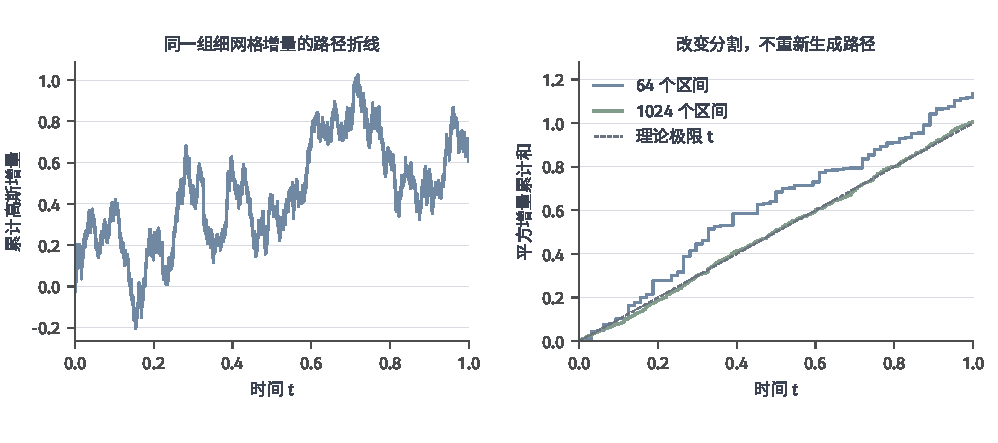
\includegraphics[width=\linewidth]{figures/02-mathematical-preliminaries-lower/01-random-variables-distributions-and-causality/matplotlib/reader-brownian-quadratic-variation/figure.pdf}
  \caption{以固定随机种子构造的高斯增量教学例。左图由$4096$个独立增量
  $\Delta W_i\sim\mathcal N(0,1/4096)$累计成路径折线；右图将同一组增量分别合并为
  $64$和$1024$个时间区间，再累计各区间增量的平方。蓝、绿阶梯线使用不同分割，
  灰色参考线为理论二次变差$t$。这里只绘制有限网格，不把某一条折线作为连续布朗路径或收敛证明。}
  \label{fig:reader-brownian-quadratic-variation}
\end{figure*}

平方增量会留下有限累计量，这使普通积分的链式法则不再适用。第~\ref{chap:dynamical-systems-and-state-estimation}章将用它建立随机积分与Itô换元。
差商在固定时刻的方差发散，是不可微的尺度提示，不是“几乎必然所有时刻都不可微”的完整证明；后者同时涉及不可数多个时刻，是严格路径定理。相应地，
\(W_{t+h}-W_t=O_{\mathbb P}(\sqrt h)\)不是对全部实现、全部短区间成立的统一确定性上界。

对同一确定分割，交叉二次变差使用增量乘积而非平方：
\[
[X,Y]_t=\lim_{|\pi|\to0}\sum_{[u,v]\in\pi}
(X_v-X_u)(Y_v-Y_u),
\]
这里按存在时的依概率极限理解。独立Brownian分量\(i\ne j\)的和均值为零，方差为
\(\sum_{[u,v]\in\pi}(v-u)^2\leq t|\pi|\)，所以
\([W^{(i)},W^{(j)}]_t=0\)；同一分量的计算则给出\(t\)。合写为
\([W^{(i)},W^{(j)}]_t=\delta_{ij}t\)。
在二进分割上，对任意固定容差，平方和偏离\(t\)的概率由上述方差界控制且可求和。尾部坏事件的并集概率因而趋零，说明沿这列分割，几乎每条实现最终都不再超过该容差。再取可数个递减容差，便得到逐个固定终点的几乎必然收敛。对一般网格列，这里的无条件结论是已证明的\(L^2\)及依概率收敛，不把它加强成对所有分割同时逐路径成立。

\subsubsection{均值与协方差约束下的高斯过程构造}
% Baseline S:41-58
布朗运动已用独立高斯增量规定时间依赖。若温度曲线相隔较近时更相似，却不满足独立增量，就不能照搬这项假设。可以保留任意有限组读数联合高斯的结构，改用均值函数和协方差函数指定它们的联系；索引也可以从时间扩大为一般输入位置。
\begin{definition}[高斯过程]
  \label{def:stoch-gaussian-process}
  实值随机过程\((F(x))_{x\in\mathcal X}\)称为\term{高斯过程}（Gaussian process），若任意正整数\(m\)及任意\(x_1,\ldots,x_m\in\mathcal X\)上的向量
  \((F(x_1),\ldots,F(x_m))^\top\)均服从多元高斯分布，允许协方差奇异。其均值函数和协方差函数为
  \[
    m(x)=\mathbb E F(x),\qquad
    k(x,x')=\operatorname{Cov}(F(x),F(x')),
  \]
  因而每个有限向量的均值为\((m(x_i))_i\)，协方差矩阵为\((k(x_i,x_j))_{i,j}\)，记作\(F\sim\mathcal{GP}(m,k)\)。索引\(x\)不必代表时间。
\end{definition}
协方差函数必须对称，且对任意有限输入和实系数\(c_i\)满足
\[
  \sum_{i,j}c_ic_jk(x_i,x_j)\geq0.
\]
这正是有限协方差矩阵半正定的条件。均值与协方差因此确定高斯过程的全部有限维分布；它们本身不自动保证样本函数连续、可微或具有Markov性。

例如令\(A,B\)是独立标准高斯变量，定义\(F(x)=A+Bx\)。任意有限函数值都是\((A,B)\)的线性变换，所以构成高斯过程，且
\(m(x)=0\)、\(k(x,x')=1+xx'\)。三个以上不同输入的协方差矩阵可以奇异，因为这些随机值都由同两个随机系数决定。反过来，各点边缘高斯并不足够：若\(X\sim\mathcal N(0,1)\)，独立符号\(S\)等概率取\(\pm1\)，则\(X,SX\)的边缘均为标准高斯且不相关，但\((SX)^2=X^2\)使它们依赖，故不可能是联合高斯。定义中的“任意有限联合分布”不可省略。
布朗运动是均值零、核\(k(s,t)=\min(s,t)\)的高斯过程：每个有限向量都由独立高斯增量线性组合得到。这个核确实半正定，因为
\[
\sum_{i,j}c_ic_j\min(t_i,t_j)
=\int_0^\infty\left(\sum_i c_i\mathbb I_{\{u\leq t_i\}}\right)^2\,\mathrm du\geq0.
\]
一般给定均值和对称半正定核时，相应高斯有限维分布相容，可用第~\ref{sec:rv-finite-dimensional-laws}节的扩张定理建立过程。要得到连续版本，仍须对核控制增量矩；“高斯过程”这个名称本身不承诺路径光滑。


\subsection{基于Dirichlet规律的随机概率测度生成}
\label{sec:stoch-random-probability-generation}
第~\ref{sec:rv-random-generation}节的层次模型让一个参数向量随机；现在把随机对象扩大为整张概率测度。它也可以看成以可测集合为索引的一族随机质量，但每条实现还须对这些集合满足可数可加性。
把空间划成有限个区域后，一个随机分布先表现为各区域的随机概率，且这些概率之和为$1$。
有限Dirichlet分布正好描述这样的概率向量。要求任意有限分割都具有彼此相容的Dirichlet
概率向量，就得到\term{Dirichlet过程}；这里增加的是随机对象的范围，而不是直接把向量维数写成无穷。
\paragraph{随机概率测度的有限分割表示}
\begin{definition}[随机概率测度]
  \label{def:probability-random-probability-measure}
在可测空间
\((\mathcal X,\mathcal A)\)上，先给概率测度空间\(\mathcal P(\mathcal X)\)配备
\term{评价$\sigma$代数}：它由全部映射
\(\mu\mapsto\mu(A)\)，\(A\in\mathcal A\)，生成。随机概率测度就是从底层概率空间到
这个可测空间的可测映射；换言之，对每个\(A\in\mathcal A\)，\(G(A)\)都必须是随机
变量。
\end{definition}
\paragraph{相容分割下的Dirichlet过程}
\begin{definition}[Dirichlet过程]
  \label{def:probability-dirichlet-process}
  设\((\mathcal X,\mathcal A)\)为标准Borel空间，\(G_0\)为其上的概率测度，\(\alpha>0\)。随机概率测度\(G\)称为参数\((\alpha,G_0)\)的Dirichlet过程，记作\(G\sim\operatorname{DP}(\alpha,G_0)\)，若对任意有限可测分割
\((A_1,\ldots,A_K)\)，
\[ (G(A_1),\ldots,G(A_K))
  \sim\operatorname{Dirichlet}(\alpha G_0(A_1),\ldots,\alpha G_0(A_K)). \]
其中\(\alpha>0\)是总质量参数，\(G_0\)是基概率测度；若
\(G_0(A_k)=0\)，则相应坐标满足\(G(A_k)=0\)几乎必然，应删除该零参数坐标后理解Dirichlet向量。
\end{definition}
这一定义通过全部有限分割刻画随机分布。合并两个分块时，概率质量相加，Dirichlet参数也相加；这说明不同分割规律彼此相容。
相容性还不足以保证每条实现都可数可加。标准Borel空间上的存在性可由随机离散测度构造证明：Ferguson把一族正的随机跳跃质量归一化，使权重和为\(1\)，再把这些权重放在独立、服从\(G_0\)的随机位置上。所得对象逐条实现都是概率测度，各有限分割质量又满足上述Dirichlet规律\scite{statistics-ferguson1973dirichlet}。
后验、聚类表示及非参数Bayes计算留给概率模型章节。

\section{随机累计量的偏差控制}
\label{sec:probability-averages-errors}
\label{sec:rv-aggregation}
用\(n\)次读数求和或取平均后，还需要判断结果偏离目标多少。我们固定\(n\)和误差阈值，控制超出阈值的概率。
控制的对象不同，所需的论证也不同：查询一个预先固定的累计量，只需保证这一个量；
从候选族中挑出累计量最小的一个，则必须让保证同时覆盖全部候选，否则选出的那个恰好
是被噪声压低的可能性没有被排除；根据历史继续收集记录，样本量与观测时刻本身也是随机的，
条件化要求随之改变。本节依次处理这三种情形。下一节再用累计量的概率保证分析采样积分。
样本数增长后的极限不能代替当前预算下的概率界。

\subsection{单个累计量的偏差控制}
\label{sec:probability-basic-tail-bounds}
\label{sec:probability-concentration-inequalities}
\subsubsection{矩条件下的尾概率控制}
固定独立样本数后，最直接的误差指标是样本平均的方差。若\(X_1,\ldots,X_n\)相互独立，且各项二阶矩有限，记\(\overline X_n=n^{-1}\sum_{i=1}^nX_i\)，则
\[
 \operatorname{Var}(\overline X_n)
 =\frac1{n^2}\sum_{i=1}^n\operatorname{Var}(X_i).
\]
第~\ref{sec:rv-features}节的Markov与Chebyshev不等式将一阶或二阶矩转成尾概率。将式~\eqref{eq:probability-chebyshev-inequality}用于这里的平均误差，得到
\[
 \mathbb P\{|\overline X_n-\mathbb E\overline X_n|\geq\varepsilon\}
 \leq\frac{\sum_i\operatorname{Var}(X_i)}{n^2\varepsilon^2},
 \qquad\varepsilon>0.
\]
同分布且单次方差为\(\sigma^2\)时，右侧为\(\sigma^2/(n\varepsilon^2)\)。这个界只利用方差；相同方差的有界变量与重尾变量可能有不同的实际尾部。若样本相关，平均方差中还要保留所有交叉协方差，不能继续把方差除以\(n\)作为通用结论。

% Baseline P:1698-1841
\subsubsection{指数矩条件下的累计偏差控制}
对任意\(\lambda>0\)，函数\(x\mapsto e^{\lambda x}\)单调。Markov不等式给出
\begin{equation}
  \mathbb{P}(X\geq t)
  =
  \mathbb{P}(e^{\lambda X}\geq e^{\lambda t})
  \leq
  e^{-\lambda t}\mathbb{E}[e^{\lambda X}].
  \label{eq:probability-chernoff-step}
\end{equation}
随后对\(\lambda\)优化，便得到Chernoff方法。整个方法依赖相应指数矩有限；若\(\mathbb{E}e^{\lambda X}=\infty\)，式
\eqref{eq:probability-chernoff-step}虽形式上仍真，却不给出有用上界。

Chernoff方法把尾概率问题转成指数矩问题。对方差为\(\sigma^2\)的中心高斯变量，指数矩恰为\(\exp(\lambda^2\sigma^2/2)\)；若另一变量的指数矩也不超过这个形式，同一优化就给出高斯型尾界。因此需要命名这类具有共同指数矩上界的变量，而无需假设它们本身是高斯。
\begin{definition}[次高斯变量]
  \label{def:probability-subgaussian}
对\(\sigma^2>0\)，均值为零的可积实随机变量\(X\)若满足
\[ \mathbb{E}[e^{\lambda X}]
  \leq\exp\left(\frac{\lambda^2\sigma^2}{2}\right),\qquad \lambda\in\mathbb{R}, \]
就称它为参数\(\sigma^2\)的\term{次高斯变量}（sub-Gaussian random variable）。
\end{definition}
对\(t>0\)，代入Chernoff界并取\(\lambda=t/\sigma^2\)，得到
\[ \mathbb{P}(X\geq t)
  \leq\exp\left(-\frac{t^2}{2\sigma^2}\right). \]
“次高斯”描述的是指数矩或尾部上界，不表示变量本身服从高斯分布。

\par\medskip\noindent\textbf{有界变量的Hoeffding不等式}\quad
实际读数可能只知道上下界，尚不知道矩母函数。要继续使用Chernoff方法，就需先从区间长度推出统一的指数矩上界。Hoeffding引理完成这一步，再由独立性把单个变量的控制合成为累计量的控制。
\begin{lemma}[Hoeffding引理]
\label{lem:probability-hoeffding-lemma}
若\(\mathbb{E}X=0\)且\(X\in[a,b]\)几乎处处成立，则
\[ \mathbb{E}[e^{\lambda X}]
  \leq\exp\left\{\frac{\lambda^2(b-a)^2}{8}\right\},\qquad \lambda\in\mathbb{R}. \]
\end{lemma}

\begin{proof}
若\(a=b\)，均值为零迫使\(X=0\)，结论直接成立。以下设\(a<b\)。
凸性说明，对\(x\in[a,b]\)，指数函数位于连接端点的弦下方：
\[ e^{\lambda x}
  \leq\frac{b-x}{b-a}e^{\lambda a}+\frac{x-a}{b-a}e^{\lambda b}. \]
取期望并使用\(\mathbb{E}X=0\)。令\(p=-a/(b-a)\in[0,1]\)、
\(s=\lambda(b-a)\)，则右侧的对数为
\[
 \psi(s)=\log\bigl[(1-p)e^{-ps}+pe^{(1-p)s}\bigr].
\]
这里对无量纲变量\(s\)求导。写
\(r_s=pe^s/(1-p+pe^s)\)，直接求导得到
\(\psi''(s)=r_s(1-r_s)\leq1/4\)，且\(\psi(0)=\psi'(0)=0\)。
Taylor积分余项给出
\(\psi(s)=s^2\int_0^1(1-u)\psi''(us)\,\mathrm du\leq s^2/8\)，
对正负\(s\)都成立。代回原变量，便有
\[ \log\mathbb{E}[e^{\lambda X}]
  \leq\frac{\lambda^2(b-a)^2}{8}. \]
指数化即得结论。
\end{proof}

\begin{theorem}[Hoeffding不等式]
\label{thm:probability-hoeffding-inequality}
设\(X_1,\ldots,X_n\)相互独立，且\(X_i\in[a_i,b_i]\)几乎处处成立。若\(\sum_i(b_i-a_i)^2>0\)，则对\(t>0\)，
\[
  \mathbb{P}\left(
    \sum_{i=1}^{n}(X_i-\mathbb{E}X_i)\geq t
  \right)
  \leq
  \exp\left\{
    -\frac{2t^2}{\sum_{i=1}^{n}(b_i-a_i)^2}
  \right\}.
\]
当全部区间宽度为零时，中心化和恒为零，上述右尾概率为零。
\end{theorem}

\begin{proof}
只需证明总区间宽度平方和为正的情形。记\(S=\sum_i(X_i-\mathbb{E}X_i)\)。对\(\lambda>0\)，独立性使指数矩分解：
\[
\begin{aligned}
  \mathbb{P}(S\geq t)
  &\leq
  e^{-\lambda t}\mathbb{E}[e^{\lambda S}]\\
  &=
  e^{-\lambda t}
  \prod_{i=1}^{n}
  \mathbb{E}\left[
    e^{\lambda(X_i-\mathbb{E}X_i)}
  \right]\\
  &\leq
  \exp\left\{
    -\lambda t+
    \frac{\lambda^2}{8}
    \sum_{i=1}^{n}(b_i-a_i)^2
  \right\}.
\end{aligned}
\]
右侧关于\(\lambda\)的最小点为
\[ \lambda^\star
  =\frac{4t}{\sum_i(b_i-a_i)^2}. \]
代回即得结论。对\(-S\)使用同一结果，再用联合界可得双侧版本。
\end{proof}

若\(X_i\in[0,1]\)独立，则对\(\varepsilon>0\)，样本平均满足
\[ \mathbb{P}(|\overline{X}_n-\mathbb{E}\overline{X}_n|
  \geq\varepsilon)\leq 2e^{-2n\varepsilon^2}. \]
有界性进入Hoeffding引理，独立性进入矩母函数乘积；删除任一条件都不能沿用这份证明。

\par\medskip\noindent\textbf{方差敏感的Bernstein不等式}\quad
Hoeffding界只看到取值区间。两种读数即使区间相同，一种几乎总在均值附近，另一种经常到达端点，实际累计波动也会不同。已知方差时，可以让它控制常见的小波动，再用幅值上限限制罕见的大增量；下面的分母同时保留这两种尺度。
若独立中心化变量满足\(|X_i|\leq M\)，其中\(M>0\)，并记\(v=\sum_i\mathbb{E}[X_i^2]\)，则对\(t>0\)，Bernstein不等式的一个版本为
\begin{equation}
  \mathbb{P}\left(\sum_{i=1}^{n}X_i\geq t\right)
  \leq
  \exp\left\{
    -\frac{t^2}{2(v+Mt/3)}
  \right\}.
  \label{eq:probability-bernstein-inequality}
\end{equation}
为看清两个尺度的来源，取\(0<\lambda<3/M\)。由指数级数及
\(|X_i|^k\leq M^{k-2}X_i^2\)（\(k\geq2\)），有
\[
  \mathbb{E}e^{\lambda X_i}
  \leq
  1+\frac{\lambda^2\mathbb{E}X_i^2}
           {2(1-\lambda M/3)}
  \leq
  \exp\left\{
    \frac{\lambda^2\mathbb{E}X_i^2}
         {2(1-\lambda M/3)}
  \right\}.
\]
这里第一阶项因中心化而消失，常数\(1/3\)来自用几何级数控制
\[
  \sum_{k\geq3}\frac{(\lambda M)^{k-2}}{k!}.
\]
独立性使各指数矩相乘，Chernoff步骤于是给出
\[
  \mathbb{P}\left(\sum_iX_i\geq t\right)
  \leq
  \exp\left\{
    -\lambda t+\frac{\lambda^2v}
      {2(1-\lambda M/3)}
  \right\}.
\]
若\(v=0\)，则全部\(X_i=0\)几乎处处，尾概率为零。若\(v>0\)，取\(\lambda=t/(v+Mt/3)\in(0,3/M)\)便得到式~\eqref{eq:probability-bernstein-inequality}。小偏差区域由\(v\)主导，呈高斯型；大偏差区域由\(Mt\)主导，呈指数型。

例如\(B_i\sim\operatorname{Bernoulli}(0.01)\)独立，考虑
\(\overline{B}_n-0.01\geq0.05\)。Hoeffding上界为
\(\exp(-0.005n)\)，而Bernstein上界约为
\[
  \exp\left\{
    -\frac{0.05^2n}
      {2(0.01\times0.99+0.05/3)}
  \right\}
  \approx \exp(-0.047n).
\]
低发生率使实际方差远小于区间最坏尺度，所以后者明显更紧；当方差接近区间允许的最大值或偏差进入线性尺度时，Bernstein并不保证处处优于Hoeffding。

对重尾变量，方差可能不存在，指数矩也可能对所有正参数发散。此时Chebyshev、Hoeffding和Bernstein各自在矩、范围或指数矩步骤失效。可以增加截断、稳健均值或仅用
有限\(p\)阶矩推导多项式尾界，但所得估计对象和偏差需要重新说明，不能继续声称高斯型集中。

\subsection{候选族累计量的统一偏差控制}
\label{sec:probability-uniform-errors-symmetry}
\label{sec:probability-random-functions-uniform-error}
设同一批记录既用于计算多个候选的平均，又要从中挑出表现最好的一个。选择规则会天然偏向那些偶然偏低的平均，所以对单个预先固定的候选成立的误差保证，未必适用于选中的候选。要让结论对选中的候选也有效，需要构造一个共同事件：在这个事件上，每个候选的累计误差都同时受控。这里上确界遍历候选函数，求和索引遍历样本；这两个范围共同决定保证的含义。

\paragraph{有限候选的联合控制}
% Baseline P:1855-1917
设有限候选类\(\mathcal{H}=\{h_1,\ldots,h_M\}\)，损失\(\ell(h,Z)\in[0,1]\)。真实风险与经验风险分别为
\[ R(h)=\mathbb{E}[\ell(h,Z)],
  \qquad\widehat{R}_n(h)=\frac{1}{n}\sum_{i=1}^{n}\ell(h,Z_i), \]
其中\(Z_1,\ldots,Z_n\)独立同分布。对预先固定的单个\(h\)，Hoeffding不等式给出
\[ \mathbb{P}\bigl(
    |\widehat{R}_n(h)-R(h)|>\varepsilon\bigr)\leq 2e^{-2n\varepsilon^2}. \]
但经验最优候选
\(\widehat{h}\in\arg\min_h\widehat{R}_n(h)\)由同一批训练样本选出，不是预先固定对象。只控制一个候选不能排除“恰好因噪声看起来最好”的选择偏差。

为明确“同时控制”与“样本量足够”的关系，把上述要求写成一个定义。这里讨论抽样前固定的函数类；所有上确界均假定可测。一项常用充分条件是存在可数子类，使每个函数都是该子类中某个序列的逐点极限。
\begin{definition}[分布无关的一致收敛]
  \label{def:uniform-convergence}
  设\(\mathcal G\)是非空的\([0,1]\)值可测函数类。若对任意\(\eta,\delta\in(0,1)\)，存在只依赖\(\mathcal G,\eta,\delta\)的整数\(n_0\)，使任意概率分布\(P\)和任意\(n\geq n_0\)的独立同分布样本\(S=(Z_1,\ldots,Z_n)\sim P^n\)均满足
  \begin{equation}
    \mathbb P_{S\sim P^n}\left\{
      \sup_{g\in\mathcal G}\left|\frac1n\sum_{i=1}^ng(Z_i)-\mathbb E_Pg\right|\leq\eta
    \right\}\geq1-\delta,
    \label{eq:uniform-convergence-definition}
  \end{equation}
  就称\(\mathcal G\)满足分布无关的\term{一致收敛}（uniform convergence）。若只要求\(P\)属于指定分布族，同一定义给出相对于该分布族的一致收敛。
\end{definition}
“函数上一致”由上确界表达，“分布无关”则要求同一个\(n_0\)适用于全部允许分布。对每个固定函数或每个固定分布分别存在的样本量，不能自动满足这两个量词。

\begin{theorem}[有限函数类的一致误差界]
\label{thm:probability-finite-class-uniform-bound}
在上述条件下，对任意\(\delta\in(0,1)\)，以至少\(1-\delta\)的概率同时对所有\(h\in\mathcal{H}\)有
\begin{equation}
  |\widehat{R}_n(h)-R(h)|
  \leq
  \sqrt{\frac{\log(2M/\delta)}{2n}}.
  \label{eq:probability-finite-class-bound}
\end{equation}
\end{theorem}

\begin{proof}
对每个\(h\)定义坏事件
\[ A_h=
  \{|\widehat{R}_n(h)-R(h)|>\varepsilon\}. \]
单函数Hoeffding界给出\(\mathbb{P}(A_h)\leq2e^{-2n\varepsilon^2}\)。由联合界，
\[ \mathbb{P}\left(\bigcup_{h\in\mathcal{H}}A_h\right)
  \leq 2M e^{-2n\varepsilon^2}. \]
令右侧等于\(\delta\)，解得\(\varepsilon=\sqrt{\log(2M/\delta)/(2n)}\)。在坏事件并集的补集上，结论对
全部候选同时成立。
\end{proof}

令\(h^\star\in\arg\min_hR(h)\)，并在式\eqref{eq:probability-finite-class-bound}成立的事件上记右侧为\(\varepsilon_n\)。则
\[
\begin{aligned}
  R(\widehat{h})
  &\leq
  \widehat{R}_n(\widehat{h})+\varepsilon_n\\
  &\leq
  \widehat{R}_n(h^\star)+\varepsilon_n\\
  &\leq
  R(h^\star)+2\varepsilon_n.
\end{aligned}
\]
第二步正是经验最优性的用途。候选数只通过\(\log M\)进入，但若候选类本身由同一批训练样本任意生成，简单地把最终数量代入\(M\)未必合法；需要把生成过程纳入统一控制对象。
例如\(M=100\)、\(n=1000\)、\(\delta=0.05\)时，式~\eqref{eq:probability-finite-class-bound}右侧约为
\[
  \sqrt{\frac{\log 4000}{2000}}\approx0.0644.
\]
这个数同时控制一百个预先固定候选，而不是给每个候选各自提供\(95\%\)保证；后一做法的联合失败概率可能远大于\(5\%\)。
% Baseline P:1974-2031

统一控制不只用于比较预测函数，也可用于同时保护一批几何查询。若把高维点随机投影到较低维，希望所有点对的距离都近似保留，就先要控制一个方向的投影长度。高斯投影的标准化平方长度是独立标准高斯平方之和，因此先建立卡方尾界，再对有限点对使用联合界。
\begin{lemma}[\(\chi^2\)变量的尾界]
  \label{lem:probability-chi-square-tail}
  若\(Z\sim\chi_k^2\)，其中\(k\)为正整数，则对每个\(x>0\)，
  \[
    \mathbb{P}\{Z-k\geq2\sqrt{kx}+2x\}\leq e^{-x},
    \qquad
    \mathbb{P}\{k-Z\geq2\sqrt{kx}\}\leq e^{-x}.
  \]
  因而对\(0<\varepsilon<1\)，
  \begin{equation}
    \mathbb{P}\left(
      \left|\frac{Z}{k}-1\right|>\varepsilon
    \right)
    \leq2\exp\left(-\frac{k\varepsilon^2}{8}\right).
    \label{eq:probability-chi-square-relative-tail}
  \end{equation}
\end{lemma}

\begin{proof}
标准高斯积分给出\(\mathbb E e^{\lambda G^2}=(1-2\lambda)^{-1/2}\)，\(\lambda<1/2\)。独立性因而给出
\[
  \log\mathbb E e^{\lambda(Z-k)}
  =\frac{k}{2}\{-2\lambda-\log(1-2\lambda)\}
  \leq\frac{k\lambda^2}{1-2\lambda},\qquad 0<\lambda<1/2.
\]
最后一步来自\(-u-\log(1-u)=\sum_{j\geq2}u^j/j\leq u^2/[2(1-u)]\)。对上尾使用Chernoff方法，取
\(\lambda=\sqrt{x}/(\sqrt{k}+2\sqrt{x})\)，便在阈值\(2\sqrt{kx}+2x\)处得到指数\(-x\)。
对下尾，用\(u-\log(1+u)\leq u^2/2\)得到
\[
  \log\mathbb E e^{-\lambda(Z-k)}\leq k\lambda^2,\qquad\lambda>0.
\]
取\(\lambda=\sqrt{x/k}\)，在阈值\(2\sqrt{kx}\)处也得到指数\(-x\)。最后取\(x=k\varepsilon^2/8\)。当\(0<\varepsilon<1\)时，两侧阈值均不超过\(k\varepsilon\)，故相对偏差事件包含于对应尾事件的并集，联合界给出式~\eqref{eq:probability-chi-square-relative-tail}。
\end{proof}

现在把单个方向的集中推广到有限点集。这一结果称为Johnson--Lindenstrauss引理：保留有限个距离所需的随机投影维数主要随点数的对数增长，而不由原始坐标数直接决定。
\begin{theorem}[高斯随机投影的距离保持]
  \label{thm:probability-johnson-lindenstrauss}
  给定抽样前固定的\(N\geq2\)个点\(\bm x_1,\ldots,\bm x_N\in\mathbb R^d\)，以及\(\varepsilon,\delta\in(0,1)\)。若\(\bm A\in\mathbb R^{k\times d}\)的元素独立服从\(\mathcal N(0,1/k)\)，且
  \[
    k\geq\frac8{\varepsilon^2}\log\frac{N(N-1)}\delta,
  \]
  则以至少\(1-\delta\)的概率，对全部\(i,j\)同时有
  \begin{equation}
    (1-\varepsilon)\|\bm x_i-\bm x_j\|_2^2
    \leq\|\bm A\bm x_i-\bm A\bm x_j\|_2^2
    \leq(1+\varepsilon)\|\bm x_i-\bm x_j\|_2^2.
    \label{eq:probability-jl-distance-preservation}
  \end{equation}
\end{theorem}
\begin{proof}
固定一个不依赖\(\bm A\)的非零向量\(\bm v\)。矩阵各行独立，每个\((\bm A\bm v)_r\)均为均值零、方差\(\|\bm v\|_2^2/k\)的高斯变量，因此
\[
  \frac{k\|\bm A\bm v\|_2^2}{\|\bm v\|_2^2}\sim\chi_k^2.
\]
引理~\ref{lem:probability-chi-square-tail}使该方向的相对平方范数失真概率不超过\(2e^{-k\varepsilon^2/8}\)。点对差至多有\(N(N-1)/2\)个；对全部非零差使用联合界，失败概率不超过\(N(N-1)e^{-k\varepsilon^2/8}\leq\delta\)。零差经任何线性投影仍为零，无须额外尾界。
\end{proof}
结论控制的是平方距离；对距离本身开方后，因子为\(\sqrt{1\pm\varepsilon}\)。点集须在投影抽样前确定，但在同时保持事件上，可以事后任选这批点中的一对查询。它不保证对观察到\(\bm A\)后任意新造的向量都保持范数；当\(k<d\)时，\(\bm A\)的非零零空间方向就给出反例。这里的常数是便于推导的充分界，也不保证所得\(k\)一定小于\(d\)。

\paragraph{无限候选的统一控制}
% Baseline P:1921-1961
无限函数类不能直接按元素做联合界。样本上的有限取值模式与覆盖网中的有限代表，提供两种有限化方法。
使用样本取值模式时，须先引入独立样本副本并进行下文的对称化，再条件于两批合并样本。此时随机符号和只由样本上的有限取值模式决定，才可对模式使用条件尾界和联合界；这种计数方法可参考
\BookChapterRef{chap:combinatorics}{卷1《数学准备：计算、分析与几何》的“集合的计数”章}。
同一个样本模式可能对应不同的真实风险，因此不能直接把前面固定候选界中的\(M\)换成当前样本的模式数。
使用覆盖网时，若每个函数都能由有限\(\varepsilon\)-网中的代表逼近，则先控制网点，再用Lipschitz性质把误差转回原函数。下面先建立后一种方法所需的误差比较，再说明对称化怎样引入随机符号。

\begin{lemma}[覆盖数的有限网控制]
  \label{lem:probability-covering-finite-net}
  设\((\mathcal{F},d)\)具有有限\(\varepsilon\)-网
  \(\mathcal{N}_\varepsilon\)，其大小为
  \(N(\mathcal{F},d,\varepsilon)\)。若随机过程
  \(\{Z_f:f\in\mathcal{F}\}\)满足
  \[
    |Z_f-Z_g|\leq Ld(f,g)
  \]
  几乎处处对所有\(f,g\)成立，并且相关上确界可测，则对任意\(t>0\)，
  \begin{equation}
    \mathbb{P}\left\{
      \sup_{f\in\mathcal{F}}|Z_f|>t+L\varepsilon
    \right\}
    \leq
    N(\mathcal{F},d,\varepsilon)
    \sup_{f\in\mathcal{F}}\mathbb{P}(|Z_f|>t).
    \label{eq:probability-covering-finite-net}
  \end{equation}
\end{lemma}

\begin{proof}
对每个\(f\)选取满足\(d(f,g_f)\leq\varepsilon\)的
\(g_f\in\mathcal{N}_\varepsilon\)。则
\[
  |Z_f|\leq |Z_{g_f}|+L\varepsilon,
\]
所以左侧坏事件包含在
\(\bigcup_{g\in\mathcal{N}_\varepsilon}\{|Z_g|>t\}\)中。对这个有限并集使用联合界
即得结论。
\end{proof}

若\(Z_f=\widehat R_n(f)-R(f)\)，且经验风险与真实风险各自关于\(d\)都是
\(L_0\)-Lipschitz，则引理中的过程常数是\(2L_0\)。因此，网格大小、离散误差
\(2L_0\varepsilon\)和单点尾界必须一起进入结论；只报告覆盖数而不验证Lipschitz传递
还不能控制原函数类。

% Baseline P:2035-2049
有些目标不是单个样本平均，而是整批记录的函数\(F(Z_1,\ldots,Z_n)\)。若替换第\(i\)个输入最多改变\(c_i\)，即
\[ \sup_{\bm{z},z_i'}
  |F(z_1,\ldots,z_i,\ldots,z_n)-F(z_1,\ldots,z_i',\ldots,z_n)|\leq c_i, \]
当\(\sum_i c_i^2>0\)时，对\(t>0\)，独立输入下的McDiarmid不等式给出
\begin{equation}
  \mathbb{P}\bigl(
    F-\mathbb{E}F\geq t
  \bigr)
  \leq
  \exp\left\{
    -\frac{2t^2}{\sum_{i=1}^{n}c_i^2}
  \right\}.
  \label{eq:probability-mcdiarmid}
\end{equation}
若全部\(c_i=0\)，则\(F\)在样本取值的乘积域上恒定，中心化后的正尾概率为零。其证明把\(F\)依次对前\(i\)个观测条件化，形成Doob鞅；每步有界差控制一个鞅增量，再使用Hoeffding型指数矩界。独立性保证逐步揭示观测时的条件结构，有界差则限制单个观测的影响。
McDiarmid不等式的完整证明见第~\ref{sec:rv-fixed-time}节：在那里把数据函数逐步揭示为Doob鞅，并说明独立输入为什么给出所需的条件范围。
% Baseline P:2053-2272
有限候选可按数量控制误差；无限类的函数在同一组观测上可能高度相似，直接计数会忽略这种结构。\term{Rademacher复杂度}提供另一种衡量方式：固定观测点后，让函数尽量对齐一组无信号的随机正负号，再对这些正负号平均。能拟合更多随机起伏的类，需要更大的同时误差代价。
\begin{definition}[经验Rademacher复杂度]
  \label{def:rademacher-complexity}
  给定非空实值可测函数类\(\mathcal G\)和样本\(S=(z_1,\ldots,z_n)\)。令\(\sigma_i\)独立且等概率取\(-1,1\)。当上确界可测且期望有限时，\term{经验Rademacher复杂度}定义为
  \begin{equation}
    \widehat{\mathfrak R}_S(\mathcal G)
    =\mathbb E_\sigma\left[\sup_{g\in\mathcal G}\frac1n\sum_{i=1}^n\sigma_i g(z_i)\right].
    \label{eq:empirical-rademacher}
  \end{equation}
\end{definition}
固定的是样本，不是使随机和最大的函数；每一组符号都允许选择不同函数。交换上确界与期望会把所有固定函数的零均值随机和平均成零，丢掉所要衡量的拟合能力。
\begin{definition}[期望Rademacher复杂度]
  \label{def:expected-rademacher-complexity}
  对\(S\sim P^n\)，\term{期望Rademacher复杂度}定义为
  \[
    \mathfrak R_n(\mathcal G)=\mathbb E_{S\sim P^n}\widehat{\mathfrak R}_S(\mathcal G).
  \]
\end{definition}
期望复杂度还平均了抽样结果，故依赖\(P\)；经验复杂度仅依赖给定样本上的函数取值。
允许函数作凸组合会增加候选函数，却未必增加它们对随机符号的最大对齐能力。
原因在于，固定符号后，经验随机和是函数取值的线性泛函：若一个组合的各项都不超过
同一个上界，非负且归一化的加权平均也不能超过它。下面把这一几何性质写成复杂度恒等式。

\begin{theorem}[凸组合的Rademacher复杂度]
\label{thm:ensemble-convex-hull}
设$S=(z_1,\ldots,z_n)$为固定样本，$n\geq1$，$\mathcal B$为非空实值可测函数类，
且在这组样本上统一有界，即存在有限$M$使$|h(z_i)|\leq M$对所有
$h\in\mathcal B$和$i$成立。令
\[
 \operatorname{conv}(\mathcal B)
 =\left\{\sum_{t=1}^T a_t h_t:
 T\geq1,\ h_t\in\mathcal B,\ a_t\geq0,\ \sum_{t=1}^T a_t=1\right\}
\]
为全部有限凸组合构成的函数类。则
\[
 \widehat{\mathfrak R}_S(\operatorname{conv}(\mathcal B))
 =\widehat{\mathfrak R}_S(\mathcal B).
\]
若样本再按$P^n$抽取，几乎必然满足上述样本有界条件，且相应样本上确界可测、期望有限，
则期望Rademacher复杂度也满足同一恒等式。
\end{theorem}

\begin{proof}
固定一组符号$\bm\sigma$。对任意有限凸组合，由$a_t\geq0$和$\sum_ta_t=1$，
\[
 \begin{aligned}
 \frac1n\sum_{i=1}^n\sigma_i\sum_{t=1}^T a_t h_t(z_i)
 &=\sum_{t=1}^T a_t
    \left(\frac1n\sum_{i=1}^n\sigma_i h_t(z_i)\right)\\
 &\leq\sup_{h\in\mathcal B}\frac1n\sum_{i=1}^n\sigma_i h(z_i).
 \end{aligned}
\]
因此凸包上的上确界不超过基类上的上确界。反向不等式来自
$\mathcal B\subseteq\operatorname{conv}(\mathcal B)$：取$T=1$即可得到任意基函数。
于是每一组符号下的两个上确界都相等。样本上的统一有界性保证随机和与其上确界有限，
对$\bm\sigma$取期望便得经验复杂度恒等式；在额外的抽样可测性与可积条件下，再对$S$
取期望即得期望复杂度结论。证明不要求函数类有限，也不要求上确界由某个函数达到。
\end{proof}

例如，只含常值函数$0$和$1$的基类，其凸包包含全部常值$c\in[0,1]$。
固定一个观测点时，正号下的最大随机和为$1$，负号下为$0$，两类的经验复杂度都为
$1/2$。候选函数从两个增加到无穷多个，但线性随机和的最坏值仍由端点决定。
这一定理只控制实值函数的随机线性和；把组合再作阈值化等非线性变换后，
需要另外分析变换后的函数类。非负性与归一化也是凸组合的条件，不能用同一等式处理
任意符号或任意尺度的线性组合。

随机符号只改变每个观测的正负方向。若还想用连续变化的随机幅度探测同一组函数取值，可以把符号换成标准高斯系数。它仍衡量函数类对无信号随机起伏的拟合能力，但随机探测规律变了，所得复杂度需单独定义。
\begin{definition}[经验高斯复杂度]
  \label{def:gaussian-complexity}
  将随机符号换成独立标准高斯系数\(\xi_i\sim\mathcal N(0,1)\)，定义
  \[
    \widehat{\mathfrak G}_S(\mathcal G)
    =\mathbb E_\xi\left[\sup_{g\in\mathcal G}\frac1n\sum_{i=1}^n\xi_i g(z_i)\right].
  \]
  相应期望高斯复杂度为\(\mathfrak G_n(\mathcal G)=\mathbb E_S\widehat{\mathfrak G}_S(\mathcal G)\)。
\end{definition}
高斯系数的符号与幅度都变化，Rademacher系数只有符号变化。二者是关于函数类的随机平均，不能按某一组系数的最大值直接比较。

双侧误差的证明常使用带绝对值版本
\[
  \widehat{\mathfrak R}^{\mathrm{abs}}_S(\mathcal G)
  =\mathbb E_\sigma\sup_{g\in\mathcal G}\left|\frac1n\sum_i\sigma_i g(z_i)\right|
  =\widehat{\mathfrak R}_S(\mathcal G\cup(-\mathcal G)),
\]
高斯版本同样定义。若\(\mathcal G=-\mathcal G\)，两种约定可直接等同；一般函数类则不能自动等同。例如只含常数函数\(g\equiv1\)的类，其不带绝对值复杂度为\(0\)；带绝对值复杂度为\(n^{-1}\mathbb E|\sum_i\sigma_i|>0\)。以下对称化沿用带绝对值约定，后续应用单侧风险界时应核对所用版本。

\par\medskip\noindent\textbf{对称化与随机函数复杂度}\quad
这些随机和怎样控制含有未知总体期望的误差？先用独立的第二批样本替代总体期望，得到两批样本平均的差；再利用每对样本交换后规律不变，引入随机正负号。对称化的作用是把未知总体量接到前面已经定义的随机函数复杂度上。
设\(\mathcal{F}\)是一族取值于\([-1,1]\)的函数，定义
\[ \Delta(\bm{Z})
  =\sup_{f\in\mathcal{F}}\left|\mathbb{E}f(Z)-\frac{1}{n}\sum_{i=1}^{n}f(Z_i)\right|. \]
引入独立同分布副本\(Z_1',\ldots,Z_n'\)。Jensen不等式给出
\[
\begin{aligned}
  \mathbb{E}_{\bm{Z}}\Delta(\bm{Z})
  &\leq
  \mathbb{E}_{\bm{Z},\bm{Z}'}
  \sup_{f\in\mathcal{F}}
  \left|
    \frac{1}{n}\sum_{i=1}^{n}
    \bigl(f(Z_i')-f(Z_i)\bigr)
  \right|.
\end{aligned}
\]
由于每对\((Z_i,Z_i')\)交换后联合分布不变，引入独立Rademacher符号\(\sigma_i\in\{-1,1\}\)不会改变差的联合分布。因此
\[
  \mathbb{E}\Delta(\bm{Z})
  \leq
  2\mathbb{E}_{\bm{Z},\bm{\sigma}}
  \sup_{f\in\mathcal{F}}
  \left|
    \frac{1}{n}\sum_{i=1}^{n}\sigma_i f(Z_i)
  \right|.
\]
右侧是带绝对值的经验Rademacher复杂度对样本取期望后的两倍。它只在观测点上考察函数类与随机符号对齐的能力，把未知总体期望转成了条件于样本的随机和。

若\(\phi_i:\mathbb{R}\to\mathbb{R}\)均为\(L\)-Lipschitz且\(\phi_i(0)=0\)，则对任意不必关于取负封闭的函数类\(\mathcal{F}\)，带绝对值的收缩不等式为
\[
  \mathbb{E}_{\bm{\sigma}}
  \sup_{f\in\mathcal{F}}
  \left|
    \sum_i\sigma_i\phi_i(f(Z_i))
  \right|
  \leq
  2L\,
  \mathbb{E}_{\bm{\sigma}}
  \sup_{f\in\mathcal{F}}
  \left|
    \sum_i\sigma_i f(Z_i)
  \right|.
\]
一般情形需要先在取值向量类中临时加入零向量，再分别控制随机和的两个方向；这一步产生因子\(2\)。若变换后的取值向量类关于取负封闭，例如
\(\mathcal{F}=-\mathcal{F}\)且每个\(\phi_i\)都是奇函数，则可去掉该因子。这个不等式允许把预测函数的复杂度传到Lipschitz损失。若损失不全局Lipschitz或相关上确界不可积，必须限制作用范围或使用其他矩条件。

标量收缩可用逐坐标替换证明。先设函数类在固定样本上的取值向量组成有限集
\(\mathcal{A}\subset\mathbb{R}^n\)，并只考虑不带绝对值的上确界。固定前
\(n-1\)个符号，把相应部分记为\(U_{\bm{a}}\)。条件于这些符号，左侧最后一个坐标的贡献为
\[
  \frac12\sup_{\bm{a}}\{U_{\bm{a}}+\phi_n(a_n)\}
  +\frac12\sup_{\bm{a}}\{U_{\bm{a}}-\phi_n(a_n)\}.
\]
取两个上确界的近似最大元\(\bm{a},\bm{b}\)，并使用
\(\phi_n(a_n)-\phi_n(b_n)\leq L|a_n-b_n|\)。按
\(a_n-b_n\)的符号选择正负方向，便得到上式不超过
\[
  \frac12\sup_{\bm{a}}\{U_{\bm{a}}+La_n\}
  +\frac12\sup_{\bm{a}}\{U_{\bm{a}}-La_n\}.
\]
从最后一个坐标向前迭代，即得到单侧收缩。对随机和的正、负两个方向分别应用该结论，再用
\(\sup|S|=\max\{\sup S,\sup(-S)\}\)时，还需要保证两个单侧上确界非负。具体地，令
\(\mathcal{A}_0=\mathcal{A}\cup\{\bm{0}\}\)。由于\(\phi_i(0)=0\)，对每组固定符号都有
\[
\begin{aligned}
  \sup_{\bm{a}\in\mathcal{A}}
  \left|\sum_i\sigma_i\phi_i(a_i)\right|
  &\leq
  \sup_{\bm{a}\in\mathcal{A}_0}
  \sum_i\sigma_i\phi_i(a_i)
  +
  \sup_{\bm{a}\in\mathcal{A}_0}
  \left(-\sum_i\sigma_i\phi_i(a_i)\right).
\end{aligned}
\]
两个单侧上确界因包含零向量而非负。分别对\(\bm{\sigma}\)与\(-\bm{\sigma}\)应用单侧收缩，再利用二者同分布，得到
\[
  \mathbb{E}_{\bm{\sigma}}
  \sup_{\bm{a}\in\mathcal{A}}
  \left|\sum_i\sigma_i\phi_i(a_i)\right|
  \leq
  2L\,
  \mathbb{E}_{\bm{\sigma}}
  \sup_{\bm{a}\in\mathcal{A}_0}
  \sum_i\sigma_i a_i
  \leq
  2L\,
  \mathbb{E}_{\bm{\sigma}}
  \sup_{\bm{a}\in\mathcal{A}}
  \left|\sum_i\sigma_i a_i\right|.
\]
这就闭合了带绝对值版本的证明。一般函数类可由有限子类逼近并使用单调极限；不可数类还须保留前述可测性条件。

线性函数类展示了这一复杂度怎样落到熟悉的范数上。设
\[
  \mathcal{F}
  =\{\,\bm{z}\mapsto\langle\bm{w},\bm{z}\rangle:
       \lVert\bm{w}\rVert_2\leq B\,\},
  \qquad \lVert\bm{Z}_i\rVert_2\leq R.
\]
由对偶范数和Jensen不等式，
\[
\begin{aligned}
  \widehat{\mathfrak{R}}_{\bm{Z}}^{\mathrm{abs}}(\mathcal{F})
  &=
  \frac{B}{n}\mathbb{E}_{\bm{\sigma}}
  \left\lVert\sum_{i=1}^{n}\sigma_i\bm{Z}_i\right\rVert_2\\
  &\leq
  \frac{B}{n}
  \left(\sum_{i=1}^{n}\lVert\bm{Z}_i\rVert_2^2\right)^{1/2}
  \leq\frac{BR}{\sqrt n}.
\end{aligned}
\]
参数范数、样本范数和样本量分别进入\(B\)、\(R\)与\(n^{-1/2}\)。机器学习理论部分会在具体损失和模型类上继续把这一期望复杂度转换为高概率泛化界。

把Rademacher符号替换为独立标准高斯变量\(g_i\)，得到高斯复杂度
\[ \mathbb{E}_{\bm{g}}
  \sup_{f\in\mathcal{F}}
  \left|\frac{1}{n}\sum_i g_i f(Z_i)\right|. \]
记上述带绝对值的经验Rademacher复杂度和高斯复杂度分别为
\(\widehat{\mathfrak{R}}_{\bm{Z}}^{\mathrm{abs}}(\mathcal{F})\)与
\(\widehat{\mathfrak{G}}_{\bm{Z}}^{\mathrm{abs}}(\mathcal{F})\)。对任意固定样本，只要这些上确界可测且期望有限，就有单向比较
\[
  \widehat{\mathfrak{R}}_{\bm{Z}}^{\mathrm{abs}}(\mathcal{F})
  \leq
  \sqrt{\frac{\pi}{2}}\,
  \widehat{\mathfrak{G}}_{\bm{Z}}^{\mathrm{abs}}(\mathcal{F}).
\]
这个方向可直接由条件Jensen不等式解释：写\(g_i=\sigma_i|g_i|\)，符号与幅度独立，且\(\mathbb E|g_i|=\sqrt{2/\pi}\)。固定符号后，随机和的绝对值上确界是幅度向量的凸函数，先对幅度平均不大于先取上确界再平均，因而\(\widehat{\mathfrak G}^{\mathrm{abs}}_S\geq\sqrt{2/\pi}\,\widehat{\mathfrak R}^{\mathrm{abs}}_S\)。

反方向一般不能只付出普适常数。设函数类在固定样本上的取值向量恰为
\(\{\bm e_i,-\bm e_i:1\leq i\leq n\}\)，其中\(\bm e_i\)为第\(i\)个坐标向量。两个上确界分别化为
\[
 \widehat{\mathfrak R}^{\mathrm{abs}}_{\bm Z}=\frac1n,\qquad
 \widehat{\mathfrak G}^{\mathrm{abs}}_{\bm Z}
   =\frac{\mathbb E\max_{i\leq n}|g_i|}{n}.
\]
符号的绝对值恒为\(1\)，高斯幅度的最大值却随\(n\)增长。其尺度可直接核对：
对任意\(t>0\)，指数和上界及Jensen不等式给出
\[
 \mathbb E\max_i|g_i|
 \leq\frac{\log(2n)}t+\frac t2
 \leq\sqrt{2\log(2n)}
 \quad\text{当 }t=\sqrt{2\log(2n)}.
\]
下界对\(n\geq3\)取\(u=\sqrt{\log n}\geq1\)。在高斯密度积分中只保留区间
\([u,u+1/u]\)，得到
\(\mathbb P(|g_1|\geq u)\geq c\,u^{-1}e^{-u^2/2}\)，其中\(c>0\)为固定常数。
于是独立性给出
\[
 \mathbb P(\max_i|g_i|\geq u)
 \geq1-\exp\{-cn^{1/2}/\sqrt{\log n}\}\longrightarrow1.
\]
用期望下界\(u\,\mathbb P(\max_i|g_i|\geq u)\)可知，两种复杂度的比为
\(\Theta(\sqrt{\log n})\)（\(n\geq2\)，有限个小\(n\)并入常数）。
因此替换复杂度时必须保留比较方向；这个例子已经排除了普适常数的反向界。

\subsection{历史依赖下累计量的偏差控制}

逐步采集记录时，下一次观测的位置或噪声尺度可以依赖已见历史。即使每个新增量在历史条件下均值为零，它们也未必独立，不能直接乘上独立样本的指数矩。鞅差的条件均值提供替代起点；累计条件方差则记录实际沿途产生了多少波动。
% Baseline S:427-437
\begin{definition}[可预测二次变差]
  \label{def:stoch-predictable-quadratic-variation}
对平方可积鞅差，定义\term{可预测二次变差}（predictable quadratic variation）
\begin{equation}
  V_t=\sum_{s=1}^{t}\mathbb{E}[X_s^2\mid\mathcal{F}_{s-1}].
  \label{eq:stoch-predictable-quadratic-variation}
\end{equation}
\end{definition}
它在每一步使用新增量到来之前可知的条件方差，因而能够记录实际噪声规模。与之不同，
$\sum_{s=1}^{t}X_s^2$是观察后的实现二次变差。Freedman界使用前者；在其他序贯估计中
也可以围绕后者构造界，但不能不加说明地互换。

\paragraph{固定时刻的误差界}
\label{sec:rv-fixed-time}
% Baseline S:489-540
若只知道每个鞅差的范围，可以把独立变量的指数矩方法逐步条件化。

\begin{theorem}[Azuma--Hoeffding不等式]
  \label{thm:stoch-azuma-hoeffding}
  设$(X_t,\mathcal{F}_t)_{t=1}^{n}$为鞅差，并且几乎必然有
  $a_t\leq X_t\leq b_t$，其中$a_t,b_t$为确定常数。令
  $S_n=\sum_{t=1}^{n}X_t$。若$\sum_t(b_t-a_t)^2>0$，则对任意$x>0$，
  \begin{equation}
    \mathbb{P}(S_n\geq x)\leq\exp\left\{
      -\frac{2x^2}{\sum_{t=1}^{n}(b_t-a_t)^2}
    \right\}.
    \label{eq:stoch-azuma-hoeffding}
  \end{equation}
若全部宽度为零，鞅差条件均值零使每个$X_t=0$几乎必然，正尾概率为零。
\end{theorem}

\begin{proof}
对总宽度平方和为正的情形，条件Hoeffding引理给出，对任意$\lambda>0$，
\[
  \mathbb{E}[
    \exp(\lambda X_t)
    \mid\mathcal{F}_{t-1}]
  \leq
  \exp\left\{
    \frac{\lambda^2(b_t-a_t)^2}{8}
  \right\}.
\]
从$t=n$开始反复使用塔式性质，得到
\[
  \mathbb{E}\exp(\lambda S_n)
  \leq
  \exp\left\{
    \frac{\lambda^2}{8}
    \sum_{t=1}^{n}(b_t-a_t)^2
  \right\}.
\]
Markov不等式于是给出
\[
  \mathbb{P}(S_n\geq x)
  \leq
  \exp\left\{
    -\lambda x+
    \frac{\lambda^2}{8}
    \sum_{t=1}^{n}(b_t-a_t)^2
  \right\}.
\]
对$\lambda$优化，取
$\lambda=4x/\sum_t(b_t-a_t)^2$，便得到式
\eqref{eq:stoch-azuma-hoeffding}。
\end{proof}

这个证明没有要求$X_t$彼此独立，只要求给定过去后均值为零，并且条件范围受控。代价是
它把每一步都按最坏范围计费。若多数时刻的条件方差很小，下一结果会给出更紧的尺度。
现在证明此前用于数据函数的McDiarmid界。设独立输入
\(X_1,\ldots,X_n\)，可测可积函数\(f\)在只改第\(i\)个坐标时满足
\(|f(x)-f(x')|\leq c_i\)。令
\[
Z_i=\mathbb E[f(X_1,\ldots,X_n)\mid X_1,\ldots,X_i],
\quad Z_0=\mathbb Ef,\quad D_i=Z_i-Z_{i-1}.
\]
这是逐步揭示输入的Doob鞅，且\(Z_n-Z_0=f-\mathbb Ef\)。固定已经揭示的
\(x_1,\ldots,x_{i-1}\)，把尚未揭示的输入积分掉，得到关于\(x_i\)的函数\(g_i(x_i)\)。
独立性保证这次积分使用同一未来分布，所以
\(|g_i(x_i)-g_i(x_i')|\leq c_i\)。
因此给定历史后，\(D_i\)落在长度至多\(c_i\)的区间中，并且条件均值为零。区间端点可以随历史变化，长度上界\(c_i\)则是事先固定的。
条件Hoeffding引理给出
\[
\mathbb E[e^{\lambda D_i}\mid\mathcal F_{i-1}]
\leq e^{\lambda^2c_i^2/8}.
\]
逐步取条件期望后，
\(\mathbb E e^{\lambda(f-\mathbb Ef)}
\leq e^{\lambda^2\sum_i c_i^2/8}\)。
若全部\(c_i=0\)，\(f\)为常量，结论直接成立。否则，对\(u>0\)，Chernoff优化取\(\lambda=4u/\sum_i c_i^2\)，得到
\[
\mathbb P(f-\mathbb Ef\geq u)
\leq\exp\left\{-\frac{2u^2}{\sum_i c_i^2}\right\}.
\]
对\(-f\)同样处理即得双侧界。若输入依赖，更改当前输入可能同时改变未来条件分布，上面的同一分布积分便不再成立；不能只检查\(f\)的坐标差分就套用结论。

\paragraph{任意时刻的同时误差界}
\label{sec:rv-anytime}
\label{sec:stoch-self-normalized-adaptive-design}
% Baseline S:448-485
固定轮次的误差界没有同时覆盖所有查看时刻，因而不能直接把轮次换成“第一次看起来足够好”的随机时刻。要分析这类规则，先研究停止是否保留鞅的平均关系；把停止限制在一个固定有限预算内，能够先得到一个不需要交换无穷极限的结论。
\begin{theorem}[有界停时的可选停止]
  \label{thm:stoch-bounded-optional-stopping}
  设$(M_t,\mathcal{F}_t)$为可积鞅，$\tau$为满足$\tau\leq n$几乎必然成立的停时。
  则
  \[
    \mathbb{E}[M_\tau]=\mathbb{E}[M_0].
  \]
\end{theorem}

\begin{proof}
写$X_t=M_t-M_{t-1}$。由于$\tau$为停时，事件
$\{\tau\geq t\}=\{\tau\leq t-1\}^{\mathrm{c}}$属于$\mathcal{F}_{t-1}$，故其指示
函数是可预测的。又因为$\tau\leq n$，
\[
  M_\tau
  =
  M_0+\sum_{t=1}^{n}\mathbb{I}\{\tau\geq t\}X_t.
\]
对每一项使用塔式性质与鞅差条件，
\[
  \mathbb{E}\!\left[
    \mathbb{I}\{\tau\geq t\}X_t
  \right]
  =
  \mathbb{E}\!\left[
    \mathbb{I}\{\tau\geq t\}
    \mathbb{E}[X_t\mid\mathcal{F}_{t-1}]
  \right]
  =0.
\]
有限求和后即得结论。
\end{proof}

定理的证明清楚标出了有界性用途：它把随机长度的和改写为固定的有限和。对几乎必然有限的无界停时，还需要
额外条件，例如鞅一致可积、停止后的变量由某个可积变量控制，或增量有界且
$\mathbb{E}\tau<\infty$。这些条件不能省略。对从$0$开始的公平随机游走，令
$\tau=\inf\{t:S_t=1\}$。该停时几乎必然有限，却有$S_\tau=1$，所以
$\mathbb{E}S_\tau=1\neq0$；这里$\mathbb{E}\tau=\infty$，不能套用有界停时定理。

这两个首达性质可以在有限区间中核对。对正整数\(m\)，令\(\sigma_m\)为游走首次到达\(1\)或\(-m\)的时刻。
从任一内部位置出发，接下来\(m+1\)步连续向右的概率为\(2^{-(m+1)}\)，且这会使游走离开区间。因此按长度\(m+1\)分块，未退出的概率有几何上界，保证\(\mathbb E\sigma_m<\infty\)。
从位置\(j\)开始，记到达右端的概率为\(p_j\)、退出时间期望为\(e_j\)。按第一步条件化，
\[
 p_j=\tfrac12(p_{j-1}+p_{j+1}),\qquad
 e_j=1+\tfrac12(e_{j-1}+e_{j+1}),
\]
边界为\(p_{-m}=0,p_1=1,e_{-m}=e_1=0\)。解这两个有限差分方程得到
\[
 p_j=\frac{j+m}{m+1},\qquad e_j=(j+m)(1-j).
\]
故\(\mathbb P_0(S_{\sigma_m}=1)=m/(m+1)\)，令\(m\to\infty\)便知
\(\mathbb P_0(\tau<\infty)=1\)。另一方面，\(\sigma_m\leq\tau\)，所以
\(\mathbb E_0\tau\geq\mathbb E_0\sigma_m=m\)对每个\(m\)成立，期望只能为无穷。
% Baseline S:633-641
尽管无界停止未必保留期望等式，非负超鞅仍能给出任意时刻的越界概率控制。
\term{Ville不等式}说明：若$L_t$为非负超鞅且
$\mathbb{E}L_0\leq1$，则对\(0<\delta<1\)，
\begin{equation}
  \mathbb{P}\left(\sup_{t\geq0}L_t\geq\frac1\delta\right)
  \leq\delta.
  \label{eq:stoch-ville}
\end{equation}
在上述有界停止证明中，把鞅差的条件均值零换为非正，便得到超鞅版本
\(\mathbb E L_{\tau\wedge n}\leq\mathbb E L_0\leq1\)。
固定\(0<a'<a=1/\delta\)，令\(\tau\)为首次满足\(L_t\geq a'\)的时刻。
非负性给出\(a'\mathbb P(\tau\leq n)\leq\mathbb E L_{\tau\wedge n}\leq1\)；
令\(n\to\infty\)，可知某时刻实际达到\(a'\)的概率不超过\(1/a'\)。
事件\(\{\sup_tL_t\geq a\}\)包含在每个较低阈值\(a'\)的越界事件中，再令\(a'\uparrow a\)，即得式~\eqref{eq:stoch-ville}。这样也涵盖上确界只被逼近、未在某个时刻取到的情形。
反演这类同时有效的检验，可以得到随时间更新的置信集合。
% Baseline S:544-631
Ville控制的是非负超鞅越界；要把它用于累计误差\(S_t\)，还须构造连接\(S_t\)与其条件方差\(V_t\)的指数超鞅。Freedman界沿这条路线，在同一时刻累计误差已大而方差预算尚小的事件上给出控制，比只使用增量范围多保留了实际波动信息。
\begin{theorem}[标量Freedman不等式]
  \label{thm:stoch-freedman}
  设$(X_t,\mathcal{F}_t)_{t\geq1}$为鞅差，且对某个$b>0$，有$|X_t|\leq b$几乎必然成立。
  令
  \[
    S_t=\sum_{s=1}^{t}X_s,\qquad
    V_t=\sum_{s=1}^{t}
      \mathbb{E}[X_s^2\mid\mathcal{F}_{s-1}].
  \]
  则对任意$x,v>0$，
  \begin{equation}
    \mathbb{P}\left(\exists t\geq1:S_t\geq x,\ V_t\leq v\right)
    \leq\exp\left\{
      -\frac{x^2}{2(v+bx/3)}
    \right\}.
    \label{eq:stoch-freedman}
  \end{equation}
\end{theorem}

\begin{proof}
对$0<\lambda<3/b$，标量不等式
\[
  \mathrm{e}^{\lambda u}
  \leq
  1+\lambda u+
  \frac{\lambda^2u^2}{2(1-\lambda b/3)},
  \qquad |u|\leq b,
  \]
与$\mathbb{E}[X_t\mid\mathcal{F}_{t-1}]=0$共同给出
\[
  \mathbb{E}[
    \mathrm{e}^{\lambda X_t}
    \mid\mathcal{F}_{t-1}]
  \leq
  \exp\left\{
    \psi(\lambda)
    \mathbb{E}[X_t^2\mid\mathcal{F}_{t-1}]
  \right\},
  \quad
  \psi(\lambda)=
  \frac{\lambda^2}{2(1-\lambda b/3)}.
\]
因此
\[
  L_t(\lambda)
  =
  \exp\{\lambda S_t-\psi(\lambda)V_t\},
  \qquad L_0(\lambda)=1,
\]
是非负超鞅。

令
\[
  \tau
  =
  \inf\{t\geq1:S_t\geq x,\ V_t\leq v\}.
  \]
对任意整数$n$，$\tau\wedge n$有界。对非负超鞅应用有界停时论证，
$\mathbb{E}L_{\tau\wedge n}(\lambda)\leq1$。在事件$\{\tau\leq n\}$上，
  \[
  L_\tau(\lambda)\geq\exp\{\lambda x-\psi(\lambda)v\}.
  \]
故
\[
  \mathbb{P}(\tau\leq n)\leq\exp\{-\lambda x+\psi(\lambda)v\}.
  \]
令$n\to\infty$，再取
$\lambda=x/(v+bx/3)$；该值位于$(0,3/b)$，代入后得到式
\eqref{eq:stoch-freedman}。
\end{proof}

若$X_1,\ldots,X_n$相互独立、中心化且$|X_t|\leq b$，并且
$\sum_{t=1}^{n}\operatorname{Var}(X_t)\leq v$，则自然滤过下的$X_t$构成鞅差，
且$V_n\leq v$确定成立。在式~\eqref{eq:stoch-freedman}中固定$t=n$便得到
\[
  \mathbb{P}(S_n\geq x)
  \leq
  \exp\left\{
    -\frac{x^2}{2(v+bx/3)}
  \right\}.
\]
这正是式~\eqref{eq:probability-bernstein-inequality}的同常数单侧Bernstein型界。
因此，Freedman界把独立变量的方差敏感界推广到了条件方差随历史变化的序贯情形。

Freedman界同时控制所有可能时刻，但事件中还限定了$V_t\leq v$。若希望得到随观测方差
自动变化的单一边界，可以把$V_t$的可能范围分成几何区间，对各区间使用不同$v$并分配
失败概率；更精细的方法直接混合不同$\lambda$。无论采用哪种构造，序贯有效性都来自
非负超鞅，而不是把固定时刻界中的$n$替换为随机停时。
用同一族失败事件\(E_t\)表示第\(t\)次查看时所用误差界被违反。表~\ref{tab:rv-viewing-time-guarantees}
比较时间量词：采用并合界合并逐次保证时，需要为各次查看分配失败概率。
\begin{table*}[htbp]
  \centering\small
  \begin{tabularx}{\linewidth}{p{22mm}p{39mm}XX}
    \toprule
    查看方式 & 受控事件 & 所需保证 & 可据此判断的范围\\
    \midrule
    事先固定\(n\) & \(E_n\) & \(\mathbb P(E_n)\leq\delta\) & 只控制预先指定的这一次查看；更换成历史决定的时刻需要另行证明。\\
    最多查看\(T\)次 & \(\bigcup_{t=1}^T E_t\) & 各次\(\mathbb P(E_t)\leq\delta_t\)，且\(\sum_{t=1}^T\delta_t\leq\delta\) & 并合界控制总失败概率；事件无须相互独立。\\
    任意时刻同时有效 & \(\bigcup_{t\geq1}E_t\) & \(\mathbb P(\bigcup_{t\geq1}E_t)\leq\delta\) & 对几乎必然有限的正整数停时\(\tau\)，仍有\(\mathbb P(E_\tau)\leq\delta\)。\\
    \bottomrule
  \end{tabularx}
  \caption{查看时刻变化下的误差保证。\(E_t\)须包含所用界的完整条件：例如Freedman事件同时要求
  \(S_t\geq x\)与\(V_t\leq v\)。非负超鞅可经Ville不等式构造同时界；有界可选停止的期望等式本身不提供这类失败概率保证。}
  \label{tab:rv-viewing-time-guarantees}
\end{table*}

% Baseline S:686-813
标量累计和把每次噪声视为同一个方向。在线性观测中，第$t$次查询带有特征
$\bm{x}_t\in\mathbb{R}^d$，观测为
\begin{equation}
  y_t=\langle\bm{x}_t,\bm{\theta}^{\star}\rangle+\eta_t.
  \label{eq:stoch-adaptive-linear-observation}
\end{equation}
允许$\bm{x}_t$根据$\mathcal{F}_{t-1}$中的历史结果选择，但要求它在$\eta_t$揭晓前
已经确定，也就是$\bm{x}_t$可预测；噪声$\eta_t$对$\mathcal{F}_t$可测。
\begin{definition}[条件次高斯噪声]
  \label{def:stoch-conditional-subgaussian}
对\(\mathcal F_t\)-可测实随机变量\(\eta_t\)，若某个$R>0$使下面的条件指数矩界对每个\(\gamma\in\mathbb R\)几乎必然成立，则称其相对于过去信息\(\mathcal F_{t-1}\)为参数\(R^2\)的条件次高斯噪声：
\begin{equation}
  \mathbb{E}[
    \exp(\gamma\eta_t)
    \mid\mathcal{F}_{t-1}]
  \leq
  \exp\left(\frac{\gamma^2R^2}{2}\right),
  \qquad \gamma\in\mathbb{R},
  \label{eq:stoch-conditional-subgaussian}
\end{equation}
\end{definition}
该条件蕴含可积性和给定过去后均值为零，并且尾部由尺度$R$控制。

后面还要把确定参数\(\gamma\)换成过去可测的随机参数，这一步需要可测逼近。
若\(\Gamma\)只取有限个有理值且对\(\mathcal F_{t-1}\)可测，在各取值事件上应用式~\eqref{eq:stoch-conditional-subgaussian}，得到
\[
 \mathbb E\!\left[
 e^{\Gamma\eta_t-R^2\Gamma^2/2}\mid\mathcal F_{t-1}
 \right]\leq1.
\]
对任意有限实值的\(\mathcal F_{t-1}\)-可测\(\Gamma\)，取有理值简单函数\(\Gamma_k\to\Gamma\)逐点逼近。
对每个\(A\in\mathcal F_{t-1}\)，非负Fatou引理给出
\[
 \mathbb E[\mathbb I_A e^{\Gamma\eta_t-R^2\Gamma^2/2}]
 \leq\liminf_k
 \mathbb E[\mathbb I_A e^{\Gamma_k\eta_t-R^2\Gamma_k^2/2}]
 \leq\mathbb P(A).
\]
这就验证了同一条件期望界仍成立，且避免对不可数多个参数的零测例外集取并。

取事先固定的正定矩阵\(\bm V_0\)。累计噪声和正则化设计矩阵分别记为
\begin{equation}
  \bm{S}_t=\sum_{s=1}^{t}\bm{x}_s\eta_s,
  \qquad
  \bm{V}_t=\bm{V}_0+\sum_{s=1}^{t}\bm{x}_s\bm{x}_s^{\top},
  \quad\bm{V}_0\succ\bm{0}.
  \label{eq:stoch-vector-sum-design}
\end{equation}
若各增量满足\(\mathbb E\lVert\bm x_t\eta_t\rVert_2<\infty\)，可预测性与条件中心化共同保证
\[
  \mathbb{E}[\bm{x}_t\eta_t\mid\mathcal{F}_{t-1}]
  =
  \bm{x}_t
  \mathbb{E}[\eta_t\mid\mathcal{F}_{t-1}]
  =\bm{0}.
\]
这时$(\bm{S}_t)$是向量鞅。特征可预测不自动保证这一可积性；下面的指数超鞅论证只需其条件指数矩控制，因此自归一化界不要求额外假定整个向量和可积。这里没有要求$\bm{x}_t$为确定向量，也没有要求不同
$\bm{x}_t$彼此独立；关键是它在当前噪声出现前已经由过去确定。

某个方向被反复观测时，$\bm{V}_t$沿该方向增大；从未被询问的方向只剩初始正则化。
因此，自然误差尺度不是统一的欧氏球，而是
\[
  \lVert\bm{S}_t\rVert_{\bm{V}_t^{-1}}
  =\sqrt{\bm{S}_t^{\top}\bm{V}_t^{-1}\bm{S}_t}.
\]
设计提供的信息越多，逆矩阵在相应方向上的权重越小。这种由随机设计自身归一化误差的形式，
称为\term{自归一化}（self-normalized）；它与第~\ref{sec:probability-monte-carlo-variance-reduction}节中用
随机权重和归一化分母构造的自归一化重要性估计不是同一个对象。

\par\medskip\noindent\textbf{混合指数超鞅与向量集中}\quad
\begin{theorem}[向量自归一化集中界]
  \label{thm:stoch-vector-self-normalized}
  在式~\eqref{eq:stoch-adaptive-linear-observation}至
  \eqref{eq:stoch-vector-sum-design}的条件下，对任意$\delta\in(0,1)$，以至少
  $1-\delta$的概率，对所有$t\geq0$同时有
  \begin{equation}
    \lVert\bm{S}_t\rVert_{\bm{V}_t^{-1}}
    \leq
    R\sqrt{
      2\log\left(
        \frac{\det(\bm{V}_t)^{1/2}}
             {\det(\bm{V}_0)^{1/2}\delta}
      \right)
    }.
    \label{eq:stoch-vector-self-normalized-bound}
  \end{equation}
\end{theorem}

\begin{proof}
固定任意$\bm{u}\in\mathbb{R}^d$。由于$\bm{x}_t$对
$\mathcal{F}_{t-1}$可测，在式~\eqref{eq:stoch-conditional-subgaussian}中取
$\gamma=\langle\bm{u},\bm{x}_t\rangle$，得到
\[
  \mathbb{E}\!\left[
    \exp\left\{
      \langle\bm{u},\bm{x}_t\rangle\eta_t
      -\frac{R^2}{2}
       \langle\bm{u},\bm{x}_t\rangle^2
    \right\}
    \middle|\mathcal{F}_{t-1}
  \right]
  \leq1.
  \]
逐步相乘可知
\[
  L_t(\bm{u})
  =
  \exp\left\{
    \langle\bm{u},\bm{S}_t\rangle
    -\frac{R^2}{2}
     \lVert\bm{u}\rVert_{\bm{V}_t-\bm{V}_0}^2
  \right\}
\]
是非负超鞅。

一个固定$\bm{u}$只能控制一个投影方向。为同时处理所有方向，取独立于数据的随机向量
$\bm{U}\sim\mathcal{N}(\bm{0},R^{-2}\bm{V}_0^{-1})$，并对
$L_t(\bm{U})$关于$\bm{U}$积分。非负性允许交换条件期望与积分，所以混合过程
$\overline L_t=\mathbb{E}_{\bm{U}}L_t(\bm{U})$仍是非负超鞅，且
$\overline L_0=1$。把高斯密度与指数中的二次项合并，配方得到
\begin{align*}
  \overline L_t
  &=
  \left(
    \frac{\det(\bm{V}_0)}
         {\det(\bm{V}_t)}
  \right)^{1/2}
  \exp\left\{
    \frac{1}{2R^2}
    \lVert\bm{S}_t\rVert_{\bm{V}_t^{-1}}^2
  \right\}.
\end{align*}
这里行列式比来自两个高斯二次型的归一化常数，而指数项来自配方后的中心移动。

对$\overline L_t$使用式~\eqref{eq:stoch-ville}，以至少$1-\delta$的概率，对所有$t$
都有$\overline L_t<1/\delta$。取对数并整理，便得到式
\eqref{eq:stoch-vector-self-normalized-bound}。
\end{proof}

证明中的各项假设承担不同作用。条件次高斯性构造每一步指数超鞅；特征可预测性允许在条件
期望中把$\bm{x}_t$视为已知；$\bm{V}_0\succ\bm{0}$使高斯混合与逆矩阵从$t=0$起有
定义。由高斯混合得到的行列式比则记录各方向相对于初始尺度的共同增长。行列式不是把每个访问次数简单相加，
因为同一方向的重复观测与新方向的首次观测提供的信息不同。


\section{基于随机采样的积分计算}
\label{sec:stoch-sampling-integrals}
给定概率规律和被积函数后，积分仍可能难以直接求出。采样计算把这一确定的积分目标改写成随机累计量，再用其均值、方差和尾概率检查有限预算下的误差。改变抽样分布、利用已知辅助均值、消去条件内随机性与消去归一化常数，会改变不同的计算环节。

\subsection{基于独立样本平均的积分计算}
\label{sec:probability-monte-carlo-variance-reduction}
% Baseline P:1518-1691
前面的偏差界把总体期望作为比较的参照；计算时也可能恰好不知道这个期望，而只能从给定分布抽样。此时用样本平均近似积分，就得到蒙特卡洛方法。需要分别核对平均是否对准原积分，以及相同样本预算下波动有多大。
目标积分可统一写成
\[ I=\mathbb{E}_P[f(X)]. \]
若能独立采样\(X_i\sim P\)，直接蒙特卡洛估计为
\[ \widehat{I}_n
  =\frac{1}{n}\sum_{i=1}^{n}f(X_i). \]
当\(\mathbb E_P|f(X)|<\infty\)时，线性性给出无偏性；若方差
\(\sigma_f^2<\infty\)，则
\[ \operatorname{Var}(\widehat I_n)=\frac{\sigma_f^2}{n}. \]
长期一致性和缩放误差分布在第~\ref{sec:rv-aggregate-limits}节统一核验。
误差的标准差按\(n^{-1/2}\)下降，与输入维数没有显式关系，但
\(\sigma_f^2\)可能随问题结构急剧增大。

以下固定教学积分
\[ I=\int_0^1x^2\,\mathrm{d}x=\frac13. \]
若\(X\sim\operatorname{Unif}(0,1)\)，直接平均\(X_i^2\)的单样本方差为
\[ \operatorname{Var}(X^2)
  =\frac15-\frac19=\frac{4}{45}. \]

\subsection{固定积分目标下的方差缩减}
原积分保持不变时，可以改变采样位置，也可以改变每个样本的贡献。两类方法都要先验证平均值仍是原积分，再比较相同样本预算下的方差；额外的计算或先验信息也属于方法的条件。

\subsubsection{基于抽样分布的方差缩减}
直接抽取均匀位置会在贡献较小的区域也花费样本。如果能多抽取贡献较大的位置，再用原概率除以新抽样概率所得的比值纠正，就可能在保持原积分的同时降低方差。前面的换测度公式正好给出所需纠正；新分布仍须覆盖原积分有贡献的区域。
若\(P\ll Q\)，权重\(w=\mathrm{d}P/\mathrm{d}Q\)，则
\[ I=\mathbb{E}_Q[w(X)f(X)]. \]
从\(Q\)采样得到无偏估计
\begin{equation}
  \widehat{I}^{\mathrm{IS}}_n
  =
  \frac{1}{n}\sum_{i=1}^{n}w(X_i)f(X_i),
  \qquad X_1,\ldots,X_n\text{独立同分布于 }Q.
  \label{eq:probability-importance-sampling}
\end{equation}
无偏性只要求乘积可积；有限方差还要求\(\mathbb{E}_Q[w^2f^2]<\infty\)。注意这里换的是抽样分布，被积函数与积分区间都没有改变；式~\eqref{eq:probability-importance-sampling}中的\(w(X_i)f(X_i)\)是对原被积函数的一个改写，而不是对另一个积分的估计。

对上述积分，取\(Q\)的密度\(q(x)=2x\)，而\(P\)为均匀分布。除零测点\(x=0\)外，\(w(x)=1/(2x)\)，于是\(w(x)f(x)=x/2\)。单样本方差变为
\[ \mathbb{E}_Q\left[\frac{X^2}{4}\right]-\frac19
  =\frac18-\frac19=\frac{1}{72}, \]
小于直接平均的\(4/45\)。这次改进来自\(Q\)把更多样本放到\(x^2\)贡献较大的区域。
并非任意改变分布都会降低方差；若\(Q\)在重要区域过轻，权重尾部反而会放大误差。

这个例子背后有一个理想基准。对固定的被积函数\(f\)，无偏改写其实不要求整个
\(P\ll Q\)，只要求\(Q\)支配有符号测度\(f\,\mathrm{d}P\)：若\(Q(A)=0\)，则
\(\int_A|f|\,\mathrm{d}P=0\)。当\(P,Q\)相对于同一测度分别有密度\(p,q\)时，这等价于
\(q(x)>0\)在\(|f(x)|p(x)>0\)处几乎处处成立。此时令
\[
  h_Q(x)=\frac{f(x)p(x)}{q(x)},\qquad q(x)>0,
\]
便有\(I=\mathbb{E}_Q[h_Q(X)]\)。若
\(0<\mathbb{E}_P|f(X)|<\infty\)，把共同参考测度记为\(\mu\)。支配条件保证\(q=0\)处的\(|f|p\)不贡献质量，而\(\int q\,\mathrm d\mu=1\)，所以Cauchy--Schwarz不等式给出
\[
  (\mathbb E_P|f(X)|)^2
  =\left(\int_{\{q>0\}}\frac{|f|p}{\sqrt q}\sqrt q\,\mathrm d\mu\right)^2
  \leq\int_{\{q>0\}}\frac{f^2p^2}{q}\,\mathrm d\mu
  =\mathbb E_Q[h_Q^2].
\]
等号要求两个因子几乎处处成比例，即\(q\)正比于\(|f|p\)。因此，在满足该支配条件的提议密度中，最小二阶矩的归一化选择为
\[
  q^\star(x)
  =
  \frac{|f(x)|p(x)}{\mathbb{E}_P|f(X)|}.
\]
它把采样质量直接放到被积函数绝对贡献大的区域。若\(f(x)=0\)而\(p(x)>0\)，则
\(q^\star(x)=0\)，所以一般并没有\(P\ll Q^\star\)，密度比\(p/q^\star\)也不必在该点
定义；但该点对\(f\,\mathrm{d}P\)没有贡献，而且不会被\(Q^\star\)采到，只需把
\(h_{Q^\star}\)定义到\(Q^\star\)-几乎处处即可。特别地，当\(f\geq0\)时，
\(q^\star=fp/I\)，且\(h_{Q^\star}(X)=I\)在\(Q^\star\)下几乎处处成立，理论方差为零。

这个分布通常不能直接执行：归一化常数就是未知积分\(I\)，而从\(fp/I\)精确采样也可能
与原问题一样困难。若还要用同一组权重估计其他被积函数，因而必须保留\(P\ll Q\)，可以
取\(q_\eta=(1-\eta)q^\star+\eta p\)，其中\(0<\eta<1\)；混入的\(p\)为所有
\(P\)-正质量区域保留严格正支持。理想分布因此只提供设计直觉；实际提议分布还必须能够
归一化、采样并计算密度，同时覆盖\(|f|p\)非零的区域。

\subsubsection{基于辅助变量的方差缩减}
另一种办法保持抽样分布不变，只调整每个样本的贡献。若有一个与目标读数共同波动、而平均值已知的辅助读数，就可减去它偏离已知均值的部分。减去的量平均为零，能否减少方差则取决于相关性和所选系数。
设\(f(X),h(X)\in L^2\)，且辅助变量\(h(X)\)的均值\(\mu_h\)已知。对任意固定实数\(\beta\)，
\[ f_\beta(X)
  =f(X)-\beta(h(X)-\mu_h) \]
仍有期望\(I\)。其方差为
\[ \operatorname{Var}(f_\beta)
  =\operatorname{Var}(f)-2\beta\operatorname{Cov}(f,h)+\beta^2\operatorname{Var}(h). \]
当\(\operatorname{Var}(h)>0\)时，最优系数为
\[ \beta^\star
  =\frac{\operatorname{Cov}(f,h)}{\operatorname{Var}(h)}. \]
对\(f(X)=X^2\)、\(h(X)=X\)与均匀\(X\)，有
\(\mu_h=1/2\)且\(\beta^\star=1\)。调整后的变量
\[ X^2-X+\frac12 \]
仍以\(1/3\)为均值，方差降为\(1/180\)。实际用同一批抽样记录估计\(\beta^\star\)时，有限样本无偏性和方差公式需要重新核对；把估计系数当成固定常数会忽略额外随机性。

\subsubsection{基于条件平均的方差缩减}
有时估计过程中还抽取了对目标不必要的额外随机量。如果给定一部分信息后，能够直接算出估计量对剩余随机性的条件平均，就可用这个平均代替再次抽样。塔式性质保证总体均值不变，全方差分解则说明被平均掉的条件内波动不会增加方差。
设\(Y\)是目标\(I\)的无偏估计，\(\mathbb{E}[Y^2]<\infty\)。对某个统计量\(T\)定义
\[ Y^\star=\mathbb{E}[Y\mid T]. \]
全期望公式给出\(\mathbb{E}Y^\star=I\)，全方差公式给出
\begin{equation}
  \operatorname{Var}(Y)
  =
  \mathbb{E}[\operatorname{Var}(Y\mid T)]
  +
  \operatorname{Var}(Y^\star)
  \geq
  \operatorname{Var}(Y^\star).
  \label{eq:probability-rao-blackwell-variance}
\end{equation}
这就是Rao--Blackwell化：在保持均值的同时，对已知信息求条件平均，消去条件内噪声。

仍以\(I=1/3\)为例。独立生成\(X,U\sim\operatorname{Unif}(0,1)\)，令
\[ Y=\mathbb{I}\{U\leq X^2\}. \]
则\(\mathbb{E}Y=1/3\)，而\(\mathbb{E}[Y\mid X]=X^2\)。因此直接平均\(X^2\)可以看成命中估计\(Y\)关于\(X\)的Rao--Blackwell化，方差从
\((1/3)(2/3)=2/9\)降为\(4/45\)。

图~\ref{fig:probability-rao-blackwell-slice}把上述条件平均解释为一条竖切片的长度。固定\(X=x\)后，只剩\(U\)在\([0,1]\)上均匀变化，命中\(U\leq x^2\)的区段长度为\(x^2\)，所以条件平均正是\(x^2\)。例如\(x=0.6\)时，再抽取一次\(U\)只会得到\(0\)或\(1\)，其条件均值却已经能够直接算成\(0.36\)。以这个均值替代额外抽取，保留了单位正方形内命中区域的面积\(1/3\)，同时去掉给定\(X\)后仍存在的条件内波动；这里并没有改变\(X\)的抽样分布。

\begin{figure*}[htbp]
  \centering
  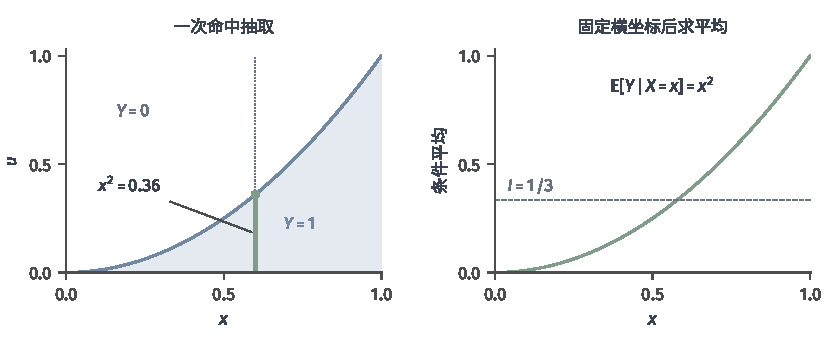
\includegraphics[width=140mm]{figures/02-mathematical-preliminaries-lower/01-random-variables-distributions-and-causality/matplotlib/probability-rao-blackwell-slice/figure.pdf}
  \caption{命中积分的Rao--Blackwell化（解析式教学图）。独立的\(X,U\)均在\((0,1)\)上均匀分布。左图阴影为\(U\leq X^2\)，竖切片\(x=0.6\)的命中长度为\(0.36\)；右图保留每个\(x\)对应的条件均值\(x^2\)。两个变量的总体期望均为\(1/3\)，但方差分别为\(2/9\)与\(4/45\)。图中没有使用随机样本估计这些量。}
  \label{fig:probability-rao-blackwell-slice}
\end{figure*}

\subsection{未知归一化常数下的积分计算}
\paragraph{自归一化权重与比值估计}
重要性估计要求能计算正确归一化的概率比。但后验密度等目标常只知道相差一个公共常数的表达。把加权读数总和除以权重总和，可以消去这个未知常数；代价是分子、分母均随机，不能再沿用线性平均的有限样本无偏结论。
设\(P\ll Q\)，但只能在未知公共常数倍的意义下计算目标密度比，即对某个\(c>0\)，
\[
  \widetilde{w}(x)
  =
  c\,\frac{\mathrm{d}P}{\mathrm{d}Q}(x),
\]
在\(Q\)-几乎处处意义下成立。对独立同分布样本\(X_i\sim Q\)，在分母为正时使用
\(\widetilde{w}_i=\widetilde{w}(X_i)\)并定义
\begin{equation}
  \widehat{I}^{\mathrm{SN}}_n
  =
  \frac{\sum_{i=1}^{n}\widetilde{w}_if(X_i)}
       {\sum_{i=1}^{n}\widetilde{w}_i}.
  \label{eq:probability-self-normalized-importance-sampling}
\end{equation}
它是两个随机平均的比值，通常在有限样本下有偏，因为一般而言
\(\mathbb E[A/B]\ne\mathbb EA/\mathbb EB\)。一致性的证明及矩条件留到第~\ref{sec:rv-aggregate-limits}节。
若\(\widetilde w\)不是目标密度比的公共常数倍，归一化权重便描述另一个加权分布，不能据此声称估计的是\(\mathbb E_Pf\)。

\paragraph{权重截断、重采样与有效样本量}
一个三点分布可以同时看清方差、截断与重采样的不同作用。令支持集为
\(\{a,b,c\}\)，提议分布和目标分布分别为
\[
  Q=(0.8,0.15,0.05),\qquad
  P=(0.4,0.3,0.3),
\]
于是重要性权重为\(w=(0.5,2,6)\)。对
\(f=(0,1,1)\)，目标均值为\(I=0.6\)。原始单样本贡献
\(Z=wf=(0,2,6)\)满足
\[
  \mathbb{E}_Q Z=0.6,\qquad
  \operatorname{Var}_Q(Z)
  =\{0.15\times4+0.05\times36\}-0.6^2
  =2.04.
\]
因此\(n\)个独立样本的无偏估计方差为\(2.04/n\)。若把权重截断在\(2\)，则
\(w^{(2)}=(0.5,2,2)\)，相应贡献的期望变为\(0.4\)，方差变为
\[
  \{0.15\times4+0.05\times4\}-0.4^2=0.64.
\]
截断降低了方差，却引入\(-0.2\)的偏差；两者必须同时报告。

再看一组恰好含\(16\)个\(a\)、\(3\)个\(b\)和\(1\)个\(c\)的二十粒子样本。
原始权重总和为\(20\)，归一化后的三点质量恰为\((0.4,0.3,0.3)\)。按这些质量做
\(20\)次多项重采样，三点后代数的条件期望为\((8,6,6)\)；重采样后无权平均的条件
期望仍为\(0.6\)，但条件方差增加了
\[
  \frac{0.6(1-0.6)}{20}=0.012.
\]
若先截断，归一化质量变成\((0.5,0.375,0.125)\)，重采样均值的条件期望是\(0.5\)，
不会恢复被截断改变的目标。原始和截断权重在这组粒子上的经验有效样本量分别约为
\(400/52=7.69\)与\(256/20=12.8\)：较均匀的权重提高了这一诊断量，但不证明偏差消失。

经验有效样本量常写成
\[ \widehat{n}_{\mathrm{eff}}
  =\frac{(\sum_i\widetilde{w}_i)^2}{\sum_i\widetilde{w}_i^2}. \]
它是权重退化的诊断量，不是对所有估计目标都成立的精确独立样本数。截断权重可降低
方差，却通常引入偏差；重采样减少后续计算中的权重不均，却增加额外随机性。本节的“自归一化”是随机比值估计，第~\ref{sec:stoch-self-normalized-adaptive-design}节的自归一化集中则用随机设计矩阵度量累计噪声，二者对象不同。

\subsection{候选函数族的采样积分误差}
对每个候选函数\(f\in\mathcal F\)，都可用同一组独立样本计算\(n^{-1}\sum_i f(X_i)\)。当计算完成后还要根据样本选择\(f\)时，单个预先固定函数的误差界不足以覆盖这一选择。第~\ref{sec:probability-uniform-errors-symmetry}节的统一偏差界直接控制\(\sup_{f\in\mathcal F}|\widehat P_n f-Pf|\)，因而同时给出整族积分近似的保证。函数类的有界性、可测性及复杂度条件仍须逐项核对；重要性权重无界时，不能直接沿用有界函数类的结论。

\subsection{历史依赖观测的轨迹重加权}
\label{sec:stoch-trajectory-reweighting}
一次积分的变量也可以是整段随机轨迹。若记录来自一种逐步生成规则，而目标平均属于另一种规则，就需要对整段联合规律换测度；单个时刻的边缘比值不足以保留历史依赖。
对有限联合观测\(X_1,\ldots,X_n\)，若在同一逐步参考核下，两个规律的条件密度分别为
\(p_i(x_i\mid x_{<i})\)、\(q_i(x_i\mid x_{<i})\)，且初始及逐步目标核对来源核绝对连续，则
\[
\frac{\mathrm dQ}{\mathrm dP}(x_{1:n})
=\prod_{i=1}^n
\frac{q_i(x_i\mid x_{<i})}{p_i(x_i\mid x_{<i})}
\quad P\text{-几乎处处}.
\]
每个比值都要条件可测，并在实际可能到达的历史上归一化；对\(P\)不可能产生而\(Q\)可能产生的观测，不能用有限权重补救。此式只依赖联合分布的链式分解，不预设Markov性。下面在共同环境中比较两种行动策略，检查哪些条件因子能够相消。

% Baseline P:1257-1273
换测度也可作用于整段观测，而不只作用于一个随机变量。考虑长度\(T\)的轨迹
\(\tau=(s_0,a_0,s_1,a_1,\ldots,s_T)\)，其中\(s_t\)记录当前状态，\(a_t\)记录当步行动。
本段取离散状态与行动，核写成条件质量函数。假定行动只按当前状态的概率核\(\pi(a_t\mid s_t)\)产生，下一状态只按
\(P(s_{t+1}\mid s_t,a_t)\)产生，且这两个核不随时间改变。
初始分布为\(\rho\)时，条件概率的链式分解给出
\[ p_\pi(\tau)
  =\rho(s_0)\prod_{t=0}^{T-1}\pi(a_t\mid s_t)P(s_{t+1}\mid s_t,a_t). \]
若目标策略为\(\pi\)，采样策略为\(\mu\)，并且两者共享同一初始分布和环境转移核，公共因子相消，得到
\begin{equation}
  \frac{p_\pi(\tau)}{p_\mu(\tau)}
  =
  \prod_{t=0}^{T-1}
  \frac{\pi(a_t\mid s_t)}{\mu(a_t\mid s_t)}.
  \label{eq:probability-trajectory-likelihood-ratio}
\end{equation}
该公式要求目标轨迹分布绝对连续于采样轨迹分布。具体地说，只要\(\pi(a\mid s)>0\)，在可能到达的状态上就需要\(\mu(a\mid s)>0\)。共同环境假设若不成立，转移核的比值也必须保留。即使每一步
比值有限，长轨迹连乘仍可能产生极大方差；密度比存在并不提供可用的二阶误差界。

\section{随机序列与过程的收敛}
\label{sec:rv-sequence-process-convergence}
有限样本偏差界固定观测次数；本节让观测次数或演化时间增长，研究所产生序列的极限。平均值、标准化累计偏差、每步状态分布及整条路径分别属于不同空间。每种极限都要同时说明生成规则、比较方式与所求对象。

\subsection{随机误差的收敛关系}
\label{sec:probability-random-convergence-asymptotics}
“越来越接近”至少有三种不同含义：几乎每一条实现都收敛到目标，大偏差事件的概率趋于零，或者整体分布逐渐逼近某个极限分布。这三种收敛不能互换。本节先建立它们之间的蕴含关系，再讨论平均和缩放波动各自趋向什么。

\subsubsection{逐次偏差与样本路径的收敛}
\label{sec:rv-numerical-convergence}
% Baseline P:1310-1444
逐个时刻的尾概率还不足以判断一条样本路径是否反复进入坏事件。记
\[
  \limsup_{n\to\infty}A_n
  =
  \bigcap_{m=1}^{\infty}\bigcup_{n\geq m}A_n,
\]
它表示事件\(A_n\)发生无穷多次。
\begin{theorem}[Borel--Cantelli引理]
  \label{thm:probability-borel-cantelli}
  对事件序列\((A_n)_{n\geq1}\)，有以下两条结论。
  \begin{enumerate}
    \item 若\(\sum_{n=1}^{\infty}\mathbb{P}(A_n)<\infty\)，则
    \(\mathbb{P}(\limsup_n A_n)=0\)；这一方向不要求独立。
    \item 若事件\(A_1,A_2,\ldots\)相互独立，且其概率之和发散，即
    \[
      \sum_{n=1}^{\infty}\mathbb{P}(A_n)=\infty,
    \]
    则\(\mathbb{P}(\limsup_n A_n)=1\)。
  \end{enumerate}
\end{theorem}

\begin{proof}
对第一条，联合界给出
\[
  \mathbb{P}\left(\bigcup_{n\geq m}A_n\right)
  \leq\sum_{n\geq m}\mathbb{P}(A_n)\longrightarrow0.
\]
而\(\limsup_n A_n\)包含在每个尾并集中，故其概率为零。对第二条，固定\(m\)。独立性
给出
\[
  \mathbb{P}\left(\bigcap_{n=m}^{N}A_n^{\mathsf c}\right)
  =
  \prod_{n=m}^{N}\{1-\mathbb{P}(A_n)\}
  \leq
  \exp\left\{-\sum_{n=m}^{N}\mathbb{P}(A_n)\right\}
  \longrightarrow0.
\]
因此从任意\(m\)开始至少有一个\(A_n\)发生的概率都为一；再对可数个\(m\)取交，
便得到\(A_n\)几乎必然发生无穷多次。
\end{proof}

\par\medskip\noindent\textbf{随机收敛的四种方式}\quad
回用定义~\ref{def:probability-random-convergence}，现在证明各收敛方式之间的关系。Markov不等式给出
\[ \mathbb{P}(|X_n-X|>\varepsilon)
  \leq\frac{\mathbb{E}[|X_n-X|^p]}{\varepsilon^p}, \]
所以\(L^p\)收敛蕴含依概率收敛。

主要蕴含关系为
\[ X_n\to_{\mathrm{a.s.}}X
  \Longrightarrow X_n\to_{\mathbb{P}}X\Longrightarrow X_n\Rightarrow X, \]
以及\(L^p\)收敛蕴含依概率收敛。前两个蕴含可以直接证明。若
\(X_n\to_{\mathrm{a.s.}}X\)，则对固定\(\varepsilon>0\)，指示变量
\(\mathbb{I}\{|X_n-X|>\varepsilon\}\)几乎处处趋于\(0\)，并由常数\(1\)控制。支配收敛定理给出
\[
  \mathbb{P}(|X_n-X|>\varepsilon)
  =\mathbb{E}\mathbb{I}\{|X_n-X|>\varepsilon\}\to0.
\]
若\(X_n\to_{\mathbb{P}}X\)，对\(F_X\)的连续点\(x\)和任意\(\varepsilon>0\)，事件包含关系给出
\[
  F_X(x-\varepsilon)-\mathbb{P}(|X_n-X|>\varepsilon)
  \leq F_{X_n}(x)
  \leq
  F_X(x+\varepsilon)+\mathbb{P}(|X_n-X|>\varepsilon).
\]
先令\(n\to\infty\)，再令\(\varepsilon\downarrow0\)，由\(F_X\)在\(x\)处连续便得
\(F_{X_n}(x)\to F_X(x)\)。

反向一般不成立。令
\(U\sim\operatorname{Unif}(0,1)\)并取
\[ X_n=\sqrt{n}\mathbb{I}\{U\leq1/n\}. \]
则\(X_n\to0\)几乎必然且依概率成立，但\(\mathbb{E}[X_n^2]=1\)，所以不均方收敛。另一方面，可以安排概率为\(1/n\)的独立
事件\(A_n\)，令\(Y_n=\mathbb{I}_{A_n}\)。此时\(Y_n\to_{\mathbb{P}}0\)，但
\(\sum_n\mathbb{P}(A_n)=\infty\)，定理~\ref{thm:probability-borel-cantelli}的第二条
说明\(A_n\)几乎必然发生无穷多次，故\(Y_n\)不几乎必然收敛到零。

依分布收敛到常数时可以推出依概率收敛到该常数；依分布收敛到非退化随机变量则通常不能。若\(X\)关于原点对称，令\(X_n=-X\)，则\(X_n\)与\(X\)同分布，却不必有\(|X_n-X|\to0\)。

虽然依概率收敛不保证整列逐路径收敛，却允许从每条子列中找到逐路径收敛的进一步子列。这使我们可以先逐条实现使用确定性极限规则，再返回概率结论。
\begin{lemma}[依概率收敛的子列判据]
 \label{lem:rv-probability-subsequence}
 对同一概率空间中的度量空间值随机变量，\(X_n\to_{\mathbb P}X\)当且仅当每条子列都有进一步子列几乎必然收敛到\(X\)。
\end{lemma}
\begin{proof}
若依概率收敛，在任意子列中递归选取指标\(n_k\)，使
\[
  \mathbb P\{d(X_{n_k},X)>2^{-k}\}\leq2^{-k}.
\]
从第\(m\)项起的偏差事件并集概率至多为\(\sum_{k\geq m}2^{-k}\)，随\(m\to\infty\)趋于零。因此几乎必然只有有限个偏差事件发生，所选子列逐路径趋于\(X\)。
反之，若不依概率收敛，则存在\(\varepsilon,\eta>0\)及一条子列，其每项都满足
\(\mathbb P\{d(X_{n_k},X)>\varepsilon\}\geq\eta\)。
它不可能有几乎必然趋于\(X\)的进一步子列，否则对偏差指示函数使用支配收敛，概率将趋于零。
\end{proof}

\subsubsection{一致尾部控制下的平均误差收敛}
只控制大多数结果上的误差，还不能交换极限与期望：极少数结果可以贡献固定的平均质量。下面的条件直接限制这种尾部贡献。
\begin{definition}[一致可积]
  \label{def:probability-uniform-integrability}
可积随机变量族\(\{X_n\}\)若满足
\[
  \lim_{K\to\infty}
  \sup_n\mathbb{E}\bigl[
    |X_n|\mathbb{I}\{|X_n|>K\}
  \bigr]=0,
\]
就称为\term{一致可积}（uniformly integrable）。
\end{definition}
它排除了越来越小概率上的巨大取值仍承载固定期望质量。若
\(X_n\to_{\mathbb P}X\)且\(\{X_n\}\)一致可积，先由一致尾界得到
\(\sup_n\mathbb E|X_n|<\infty\)。选一个几乎必然收敛的子列，再用Fatou引理，便有\(X\in L^1\)。
令\(T_K(x)=\max\{-K,\min\{x,K\}\}\)，把误差拆成
\[
\begin{aligned}
\mathbb E|X_n-X|
 &\leq\mathbb E|X_n-T_K(X_n)|\\
 &\quad+\mathbb E|T_K(X_n)-T_K(X)|\\
 &\quad+\mathbb E|T_K(X)-X|.
\end{aligned}
\]
第一项由一致可积性随\(K\)增大而统一趋零，第三项由\(X\)可积趋零。
固定\(K\)后，从任意子列用引理~\ref{lem:rv-probability-subsequence}抽取几乎必然收敛的进一步子列；截断函数连续且中间差值不超过\(2K\)，故支配收敛使中项在该子列上趋零。若整列中项不趋零，就能选出始终大于某个正数的子列，与上述结论矛盾。
因此先令\(n\to\infty\)、再令\(K\to\infty\)，得到
\(\mathbb E|X_n-X|\to0\)。没有一致可积性，例如
\(V_n=n\mathbb{I}\{U\leq1/n\}\)虽几乎必然趋于\(0\)，却满足
\(\mathbb{E}V_n=1\)，小概率上的大幅值会阻止期望收敛。

图~\ref{fig:probability-vanishing-spikes}把这个反例画在同一个基础结果\(U\)上。尖峰变高时，其底宽按相同比例缩小；每条曲线下的面积仍是\(1\)。对任何固定\(K\)，只要\(n>K\)，全部面积都位于\(V_n>K\)的尾部，因此一致可积定义中的\(\sup_n\)不能趋于零。这里失败的是对整个变量族的统一尾部控制，而不是每条样本路径的收敛。
\begin{figure*}[htbp]
  \centering
  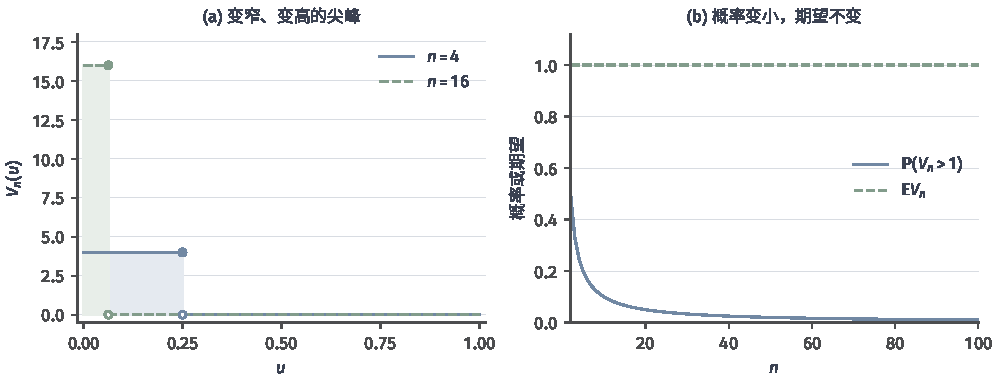
\includegraphics[width=\linewidth]{figures/02-mathematical-preliminaries-lower/01-random-variables-distributions-and-causality/matplotlib/probability-vanishing-spikes/figure.pdf}
  \caption{小概率尖峰与期望质量（解析式教学图）。左图为\(V_n(u)=n\mathbb I\{u\leq1/n\}\)在\(n=4,16\)时的取值，均以面积\(1\)贡献期望；右图对\(n\geq2\)显示\(\mathbb P(V_n>1)=1/n\)趋于零，而\(\mathbb E V_n=1\)不变。基础变量为\(U\sim\operatorname{Unif}(0,1)\)。}
  \label{fig:probability-vanishing-spikes}
\end{figure*}
\subsubsection{历史条件均值约束下的序列收敛}
鞅关系约束每一步的条件均值，但是否存在长期极限仍需条件。非负超鞅的上穿论证给出一个基本结论。设$(L_t)$为非负超鞅且
$\mathbb{E}L_0<\infty$。对任意有理数$0<a<b$，记$U_n[a,b]$为
$L_0,\ldots,L_n$从不高于$a$到不低于$b$的完整上穿次数。在每次不高于$a$时持有一单位
过程、达到$b$时卖出；由于$(L_t)$是超鞅，这个可预测交易策略的期望收益不大于$0$。
比较每次完整交易至少$b-a$的路径收益与最后一次未完成交易，得到Doob上穿不等式
\[
  (b-a)U_n[a,b]
  \leq
  \text{交易收益}+(L_n-a)^-,
  \qquad x^-:=\max\{-x,0\}.
\]
其中负部$(L_n-a)^-$至多为$a$，而交易收益的期望不大于$0$。取期望得到
\[
  (b-a)\mathbb{E}U_n[a,b]
  \leq
  \mathbb{E}(L_n-a)^-
  \leq
  a.
\]
令$n\to\infty$可知每个正有理区间几乎必然只被上穿有限次。若$L_t$的下极限严格小于上
极限，就能在二者之间选到一个正有理区间并产生无穷多次上穿，形成矛盾。因此$L_t$几乎必然
存在扩展实数极限；再由Fatou引理与
$\sup_t\mathbb{E}L_t\leq\mathbb{E}L_0<\infty$排除极限为正无穷。于是非负超鞅几乎
必然收敛到有限随机变量。这个结论只保证路径极限存在；若还要交换极限与期望，仍需一致
可积等额外条件。
非负性不是鞅收敛的唯一入口。对有正有负的累计误差，常能控制的是二阶矩。
\begin{theorem}[二阶矩有界鞅的收敛]
\label{thm:rv-l2-martingale-convergence}
若\((M_n,\mathcal F_n)\)是平方可积鞅且
\(\sup_n\mathbb E M_n^2<\infty\)，则存在\(M_\infty\in L^2\)，使
\(M_n\to M_\infty\)几乎必然且在\(L^2\)中成立，并且
\(M_n=\mathbb E[M_\infty\mid\mathcal F_n]\)。
\end{theorem}
\begin{proof}
对\(m\geq n\)，条件均值性质给出
\(\mathbb E[M_n(M_m-M_n)]=0\)，所以
\[
\mathbb E(M_m-M_n)^2=\mathbb EM_m^2-\mathbb EM_n^2.
\]
右侧来自单调有界数列，故\(M_n\)在\(L^2\)中Cauchy，有\(L^2\)极限\(M_\infty\)。
还需将均方极限提升到整条序列的几乎必然极限。对有限鞅\(Y_j\)及
\(Y^*=\max_{j\leq N}|Y_j|\)，按首次越过水平\(a\)的时刻分解事件，并用
\(|Y_j|\leq\mathbb E[|Y_N|\mid\mathcal F_j]\)，得
\[
a\,\mathbb P(Y^*\geq a)
\leq\mathbb E[|Y_N|\mathbb I_{\{Y^*\geq a\}}].
\]
积分并用Cauchy--Schwarz，得到
\[
\begin{aligned}
 \mathbb E(Y^*)^2
 &\leq2\mathbb E(|Y_N|Y^*)\\
 &\leq2\|Y_N\|_2\|Y^*\|_2,
\end{aligned}
\]
故\(\mathbb E(Y^*)^2\leq4\mathbb E Y_N^2\)。
把它用于从\(n\)起的差鞅，再令有限终点趋于无穷，有
\[
\mathbb P\left\{\sup_{m\geq n}|M_m-M_n|>\varepsilon\right\}
\leq\frac4{\varepsilon^2}
\bigl(\mathbb EM_\infty^2-\mathbb EM_n^2\bigr).
\]
取子列\(n_k\)，使括号小于\(2^{-4k}\)，并取\(\varepsilon=2^{-k}\)，坏事件概率可求和。Borel--Cantelli表明整列几乎必然Cauchy，极限与\(L^2\)极限一致。
最后对\(A\in\mathcal F_n\)，令\(m\to\infty\)于
\(\mathbb E[M_m\mathbb I_A]=\mathbb E[M_n\mathbb I_A]\)，得到所述条件期望表示。
\end{proof}
随机逼近将用平方可和步长控制累计鞅噪声；状态本身是否收敛，还要结合稳定性与漂移，不能只用这一定理替代。

\subsection{重复采样下的平均序列收敛}

每增加一个独立读数，都把累计和除以新的样本数，得到\(\overline X_n=n^{-1}\sum_{i=1}^nX_i\)。所求极限是单次读数的总体均值。前面的有限预算界可以支持部分依概率结论；要使几乎每条无限实现都收敛，还需核对相应的大数定律条件。
\label{sec:rv-aggregate-limits}
% Baseline P:1448-1511
\begin{theorem}[强大数定律]
\label{thm:probability-strong-law-large-numbers}
若\(X_1,X_2,\ldots\)独立同分布，且\(\mathbb{E}[|X_1|]<\infty\)，则
\[ \overline{X}_n
  =\frac{1}{n}\sum_{i=1}^{n}X_i\to_{\mathrm{a.s.}}\mathbb{E}[X_1]. \]
\end{theorem}

强大数定律说明同一分布下的独立重复观测，其平均几乎必然接近期望。有限方差是许多初等证明使用的方便条件，但独立同分布版本的结论只需有限一阶绝对矩。若观测相关、分布随
时间变化或样本由自适应规则收集，则不能直接引用该定理；第~\ref{sec:stoch-markov-long-run-average}节给出相关过程的一组替代条件\scite{math-kallenberg2021probability}。

有限方差时，较弱的依概率结论可以在这里完整得到。若
\(\operatorname{Var}(X_1)=\sigma^2<\infty\)，独立性使
\[
  \operatorname{Var}(\overline{X}_n)
  =\frac{1}{n^2}\sum_{i=1}^{n}\operatorname{Var}(X_i)
  =\frac{\sigma^2}{n}.
\]
把式~\eqref{eq:probability-chebyshev-inequality}用于样本平均，有
\[
  \mathbb{P}\bigl(
    |\overline{X}_n-\mathbb{E}X_1|\geq\varepsilon
  \bigr)
  \leq\frac{\sigma^2}{n\varepsilon^2}\to0.
\]
这证明了有限方差版本的弱大数定律。强大数定律只要求有限一阶绝对矩，但其证明还需截断大取值、控制截断变量的独立和，并把可求和坏事件转成几乎必然结论；不能由上面的逐个\(n\)概率界直接推出。

对例~\ref{ex:probability-noisy-observation}中的独立同分布噪声，只要\(\mathbb{E}|\varepsilon_i|<\infty\)，便有
\[ \overline{Y}_n
  =\theta+\frac{1}{n}\sum_{i=1}^{n}\varepsilon_i\to_{\mathrm{a.s.}}\theta. \]
这回答了“多测几次再平均是否稳定”，但没有给出固定\(n\)时误差超过指定阈值的概率。

\subsection{重复采样下的标准化累计偏差序列分布收敛}

平均值接近总体均值后，仍可考察剩下的随机波动。先从累计和中减去\(n\mu\)，再除以独立累计的标准差\(\sigma\sqrt n\)，得到\((\sum_{i=1}^nX_i-n\mu)/(\sigma\sqrt n)\)。这个序列通常不趋于一个固定数；在下面的条件下，它的分布趋于标准高斯。
\label{sec:rv-standardized-sum-limits}
\begin{theorem}[Lindeberg--L\'evy中心极限定理]
\label{thm:probability-iid-central-limit}
若\(X_1,X_2,\ldots\)独立同分布，\(\mathbb{E}X_1=\mu\)，\(0<\operatorname{Var}(X_1)=\sigma^2<\infty\)，则
\[ \frac{\sqrt{n}(\overline{X}_n-\mu)}{\sigma}
  \Rightarrow\mathcal{N}(0,1). \]
\end{theorem}

大数定律研究未缩放误差是否趋于零，中心极限定理研究乘以\(\sqrt{n}\)后的剩余波动近似什么分布。它给出渐近近似，而不是每个有限\(n\)都精确服从高斯分布。若方差
无限、样本依赖过强或分布随\(n\)变化而不满足相应Lindeberg条件，\(\sqrt{n}\)缩放与高斯极限都可能失效。

证明的关键是特征函数。令\(Y_i=(X_i-\mu)/\sigma\)，并记
\(\varphi(t)=\mathbb{E}e^{\mathrm{i}tY_1}\)。复指数绝对值恒为\(1\)，所以特征函数总有定义。由
\(\mathbb{E}Y_1=0\)、\(\mathbb{E}Y_1^2=1\)及零点处的二阶展开，
\[
  \varphi(u)=1-\frac{u^2}{2}+o(u^2),
  \qquad u\to0.
\]
独立性使标准化和的特征函数分解为
\[
  \mathbb{E}\exp\left\{
    \mathrm{i}t\frac{1}{\sqrt n}\sum_{i=1}^{n}Y_i
  \right\}
  =
  \left[\varphi\left(\frac{t}{\sqrt n}\right)\right]^n
  \longrightarrow e^{-t^2/2}.
\]
右侧是标准高斯的特征函数，并且在零点连续。定理
~\ref{thm:probability-levy-continuity}于是给出依分布收敛。第
~\ref{sec:statistics-intervals-quantiles}节使用这个渐近分布构造近似区间，但有限样本覆盖
仍需额外误差控制，不能只引用极限式。
\subsection{随机误差变换后的极限}
\label{sec:stoch-random-transform-limits}
样本平均的极限并不是所有计算的最终输出：归一化会引入随机分母，非线性变换还会改变误差尺度。先检查随机余项的大小，再传递连续变换和常数极限，才能判断新输出的长期波动。

\subsubsection{概率阶运算与随机误差的组合}
为控制非线性变换中的乘积余项，再核对两条概率阶规则。若\(Z_n\xrightarrow{\mathrm d}Z\)，对任意
\(\epsilon>0\)，可取充分大的\(M\)使
\(\mathbb{P}(|Z|\geq M)<\epsilon/2\)。依分布收敛的闭集上界给出
\[
  \limsup_{n\to\infty}\mathbb{P}(|Z_n|\geq M)
  \leq \mathbb{P}(|Z|\geq M)<\epsilon/2,
\]
所以\(Z_n=O_{\mathbb{P}}(1)\)。此外，若
\(A_n=o_{\mathbb{P}}(1)\)、\(B_n=O_{\mathbb{P}}(1)\)，则对任意
\(\eta,\epsilon>0\)，先取\(M\)使大样本下
\(\mathbb{P}(|B_n|>M)<\epsilon/2\)，再取充分大的\(n\)使
\(\mathbb{P}(|A_n|>\eta/M)<\epsilon/2\)。于是
\[
  \mathbb{P}(|A_nB_n|>\eta)
  \leq
  \mathbb{P}(|B_n|>M)
  +\mathbb{P}(|A_n|>\eta/M)
  <\epsilon,
\]
即\(o_{\mathbb{P}}(1)O_{\mathbb{P}}(1)=o_{\mathbb{P}}(1)\)。


\subsubsection{连续变换与随机因子的极限传递}
若样本平均趋近一个非零常数，取倒数是否仍趋近该常数的倒数，取决于极限处的连续性。一般连续变换先沿逐条实现传递极限；依概率和依分布的结论再分别使用子列判据与闭集概率控制。
\begin{theorem}[连续映射]
\label{thm:rv-continuous-mapping}
若\(X_n\to X\)几乎必然或依概率，且可测函数\(g\)在\(X\)的取值处几乎必然连续，则\(g(X_n)\to g(X)\)具有相应收敛方式。
若\(X_n\Rightarrow X\)且\(\mathbb P(X\in D_g)=0\)，其中\(D_g\)为\(g\)的不连续点集，则\(g(X_n)\Rightarrow g(X)\)。变量可取值于Polish空间。
\end{theorem}
\begin{proof}
几乎必然情形逐条在连续点应用确定序列的极限规则。依概率情形使用子列判据：每个子列都有一个几乎必然收敛的子子列，应用前一结论，再用同一判据返回依概率收敛。依分布情形对闭集\(C\)，有
\(\overline{g^{-1}(C)}\subseteq g^{-1}(C)\cup D_g\)；定理~\ref{thm:rv-portmanteau}的闭集上界给出
\(\limsup_n\mathbb P(g(X_n)\in C)\leq\mathbb P(g(X)\in C)\)，即得结论。
\end{proof}
例如倒数映射在零不连续；只有极限以概率一非零时才可直接取倒数。均方收敛不能对任意连续函数自动传递，因为变换可能放大尾部。
% Baseline T:562-634
\begin{theorem}[Slutsky定理]
  \label{thm:statistics-slutsky}
  若\(X_n\xrightarrow{\mathrm d}X\)，且
  \(Y_n\xrightarrow{\mathbb{P}}c\)，其中\(c\)为常数，则
  \[
    X_n+Y_n\xrightarrow{\mathrm d}X+c,\qquad
    X_nY_n\xrightarrow{\mathrm d}cX.
  \]
  若\(c\neq0\)，还有
  \(X_n/Y_n\xrightarrow{\mathrm d}X/c\)。比值在\(Y_n=0\)的事件上可补为任意固定值；这些事件的概率趋于零，因而不影响该分布极限。特别地，若
  \(R_n=o_{\mathbb{P}}(1)\)，则
  \(X_n+R_n\xrightarrow{\mathrm d}X\)。
\end{theorem}

\begin{proof}
先证明和的结论。任取\(\varepsilon>0\)，记\(p_n=\mathbb P(|Y_n-c|>\varepsilon)\)。事件包含关系给出
\[
 F_{X_n}(x-c-\varepsilon)-p_n
 \leq F_{X_n+Y_n}(x)
 \leq F_{X_n}(x-c+\varepsilon)+p_n.
\]
在\(F_{X+c}\)的连续点\(x\)，先令\(n\to\infty\)，再沿使两端均为\(F_X\)连续点的\(\varepsilon\downarrow0\)，得到\(F_{X_n+Y_n}(x)\to F_{X+c}(x)\)。

依分布收敛使\(X_n=O_{\mathbb P}(1)\)，而\(Y_n-c=o_{\mathbb P}(1)\)，故前面的概率阶规则给出\(X_n(Y_n-c)=o_{\mathbb P}(1)\)。将
\(X_nY_n=cX_n+X_n(Y_n-c)\)代入刚证明的和的结论，并对\(cX_n\)应用连续映射，即得乘积结论，包括\(c=0\)的退化情形。若\(c\neq0\)，连续映射还使\(1/Y_n\to_{\mathbb P}1/c\)，再用乘积结论得到比值。零分母事件包含在\(\{|Y_n-c|\geq|c|\}\)中，概率趋于零，因此该事件上的约定不影响极限。
\end{proof}

Slutsky定理允许把收敛到常数的标准误、归一化因子或余项代入渐近分布。它不表示两个一般
随机极限可以忽略联合分布；关键条件是其中一个序列依概率收敛到常数。

均值的标准误估计若依概率趋向正确的正尺度，Slutsky定理就允许在渐近统计量中代入它。条件是标准误的随机极限正确，不能由一次算出的数值看起来合理来代替。非线性函数的缩放误差将在定理~\ref{thm:statistics-delta-method}中进一步用Taylor展开处理。
% Baseline T:636-743
现在可以回到第~\ref{sec:probability-monte-carlo-variance-reduction}节，逐项核验积分近似的长期条件。直接平均只要
\(\mathbb E|f(X)|<\infty\)就强一致，若再有有限正方差，则中心极限定理给出
\(\sqrt n(\widehat I_n-I)\Rightarrow\mathcal N(0,\operatorname{Var}(f(X)))\)。
重要性采样把\(f(X)\)换成\(w(X)f(X)\)，因此要在来源分布下分别查
\(\mathbb E|wf|\)和\(\mathbb E[(wf)^2]\)；密度比存在并不推出第二项有限。

控制变量使用预先固定的系数及已知均值时，同样对修正后的被积量检查一阶、二阶矩。若系数由同一数据估计，无偏性可能不再成立；在系数一致、控制变量有适当矩等条件下，可用Slutsky分析其余项，不能直接照搬固定系数公式。Rao--Blackwell化的条件期望保留一阶可积性，在二阶可积时又由条件Jensen不等式不增方差。

自归一化重要性估计是两个平均的比。设非归一化权重\(\widetilde w\geq0\)，
\(0<Z=\mathbb E_Q\widetilde w<\infty\)，且
\(\mathbb E_Q|\widetilde wf|<\infty\)。沿用\(\widetilde w/Z=\mathrm dP/\mathrm dQ\)
及独立同分布的\(Q\)样本，两个强大数定律和连续映射给出
\[
\frac{\sum_i\widetilde w(X_i)f(X_i)}
{\sum_i\widetilde w(X_i)}
\longrightarrow
\frac{\mathbb E_Q[\widetilde wf]}Z=I
\quad\text{几乎必然}.
\]
分母由强大数定律最终远离零。若
\(\mathbb E_Q[\widetilde w^2(1+f^2)]<\infty\)，可把中心化比值直接写成
\[
 \sqrt n(\widehat I_{\mathrm{SN}}-I)
 =\frac{n^{-1/2}\sum_{i=1}^n
       \widetilde w(X_i)(f(X_i)-I)}
       {n^{-1}\sum_{i=1}^n\widetilde w(X_i)}.
\]
分子的求和项独立同分布，均值为零，方差为
\(\mathbb E_Q[\widetilde w^2(f-I)^2]\)。方差为正时，标量中心极限定理给出分子的高斯极限；分母强收敛到\(Z>0\)，再用Slutsky定理，得到渐近方差
\[
\frac{\mathbb E_Q[\widetilde w^2(f-I)^2]}{Z^2}.
\]
若该方差为零，分子各项几乎必然为零，极限相应退化为零常量。
这没有消除有限样本比值偏差。固定阈值截断权重通常收敛到截断后的目标；若希望阈值随样本量增长而仍恢复原积分，还要证明被截去尾部和随机误差同时消失。

\subsubsection{非线性变换后的渐近波动}
连续映射保证变换后的结果趋近目标，但没有说明误差乘以何种尺度后仍有非退化极限。若原误差具有高斯极限，局部线性近似会把变换的导数带入渐近方差。

\begin{theorem}[Delta方法]
\label{thm:statistics-delta-method}
若
\(\sqrt n(\widehat\theta_n-\theta)\xrightarrow{\mathrm d}\mathcal N(0,V)\)，
且\(g\)在\(\theta\)处可微，则
\[
  \sqrt n\bigl(g(\widehat\theta_n)-g(\theta)\bigr)
  \xrightarrow{\mathrm d}
  \mathcal N\bigl(0,g'(\theta)^2V\bigr).
\]
\end{theorem}

\begin{proof}
记
\[
  Z_n=\sqrt n(\widehat\theta_n-\theta),
  \qquad
  Z\sim\mathcal N(0,V).
\]
前面已证明依分布收敛推出概率有界，以及\(o_{\mathbb P}(1)O_{\mathbb P}(1)=o_{\mathbb P}(1)\)，故\(Z_n=O_{\mathbb P}(1)\)。

特别地，
\(\widehat\theta_n-\theta=n^{-1/2}Z_n=o_{\mathbb{P}}(1)\)，所以估计量依概率一致。
Taylor展开给出
\[
  g(\widehat\theta_n)-g(\theta)
  =g'(\theta)(\widehat\theta_n-\theta)
   +r_n(\widehat\theta_n-\theta),
\]
其中一致性与可微性保证\(r_n=o_{\mathbb{P}}(1)\)。乘以\(\sqrt n\)后，
余项是
\(r_nZ_n=o_{\mathbb{P}}(1)\)。主项由假设依分布收敛，再用Slutsky定理即得结论。
\end{proof}

例如若某估计量满足
\(\sqrt n(\widehat\theta_n-\theta)\Rightarrow\mathcal N(0,\sigma^2)\)，且
\(\theta>0\)，取\(g(\theta)=\log\theta\)，其渐近方差为
\(\sigma^2/\theta^2\)。估计量以趋于一的概率落在正半轴；在非正事件上任取一个约定值不影响极限。
若\(g'(\theta)=0\)，一阶Delta方法仍成立，但只给出零方差的退化极限；要描述非退化波动，需要更高阶展开与新的缩放。若\(g\)在目标点不可微，才不能直接应用上述定理。

\paragraph{方差稳定化与逆变换偏差}
不同均值的计数往往具有不同的方差。若希望在统一的误差尺度上处理这些读数，需要选取一种非线性变换，使变换后的渐近方差尽量不依赖未知均值。设独立同分布观测的均值为\(\mu\)，方差为已知函数形式\(V(\mu)>0\)，并且样本平均满足
\[
 \sqrt n(\overline X_n-\mu)\Rightarrow\mathcal N(0,V(\mu)).
\]
Delta方法使\(g(\overline X_n)\)的渐近方差变为\(g'(\mu)^2V(\mu)\)。因此在\(V\)正且连续的区间上，取
\begin{equation}
 g(x)=\int^x\frac{1}{\sqrt{V(u)}}\,\mathrm du,
 \qquad
 \sqrt n\{g(\overline X_n)-g(\mu)\}
 \Rightarrow\mathcal N(0,1),
 \label{eq:stoch-variance-stabilizing-delta}
\end{equation}
就得到\term{方差稳定化变换}（variance-stabilizing transform）。积分下限只改变常数偏移，不改变导数和误差方差；均值须处在所用区间内部，以保证局部展开有效。这是关于渐近波动的结论，不宣称有限样本方差精确相同。

Poisson观测满足\(V(\mu)=\mu\)。在\(\mu>0\)处，上式给出\(g(x)=2\sqrt x\)；若\(\mu=0\)，观测恒为零，不能沿用这里的非退化高斯极限。对单次均值很大的计数\(Y\sim\operatorname{Poisson}(\lambda)\)，局部Taylor近似同样给出
\(\operatorname{Var}(g(Y))\approx g'(\lambda)^2\lambda=1\)。进一步的高阶修正得到常用Anscombe变换
\[
 A(Y)=2\sqrt{Y+3/8}.
\]
其中\(3/8\)不是一阶Delta方法本身推出的常数，而是改善方差近似的修正；低计数时仍不能把离散变换结果视为精确的单位方差高斯读数\scite{vision-anscombe1948}。

对第~\ref{sec:rv-combinations}节的信号相关噪声模型，令\(Y=\alpha K+\varepsilon\)，其中\(\alpha>0\)、\(\mu\geq0\)、\(K\sim\operatorname{Poisson}(\mu/\alpha)\)，\(\varepsilon\sim\mathcal N(0,\sigma^2)\)，并假定二者独立，则
\(\mathbb EY=\mu\)、\(\operatorname{Var}(Y)=\alpha\mu+\sigma^2\)。同一导数条件给出
\[
 g(y)=\frac2\alpha\sqrt{\alpha y+\sigma^2}.
\]
这说明平方根形式如何承接线性变化的方差。该局部近似要求均值处于根号内为正且相对波动足够小的区域；高斯噪声可能使实际读数落到\(\alpha y+\sigma^2<0\)处。若对这类读数截断后再变换，就已改变变换规则及其误差，需另行核验，不能把上式当作全实轴上的精确稳定化。

逆变换也必须区分输入对象。未经处理的读数满足\(A^{-1}(A(Y))=Y\)，代数逆并不改变原读数的均值。但若在变换域平滑后，输出接近的是\(m(\lambda)=\mathbb E_\lambda A(Y)\)，则恢复\(\lambda\)需要反演函数\(m\)，不是直接对这个均值应用\(A^{-1}\)。这里甚至可以精确计算两者的差别：由于\(A(Y)^2=4Y+3/2\)，
\begin{equation}
 A^{-1}(m(\lambda))
 =\frac{m(\lambda)^2}{4}-\frac38
 =\lambda-\frac14\operatorname{Var}_\lambda(A(Y)).
 \label{eq:stoch-anscombe-inverse-bias}
\end{equation}
当\(\lambda>0\)时，右端严格小于\(\lambda\)。若变换后方差约为一，偏差便约为\(-1/4\)；变换域的平均估计即使准确，代数逆仍会引入这一系统偏移。按\(m(\lambda)\mapsto\lambda\)建立的校正逆能够消除此处由均值映射造成的偏差，但对带有额外估计误差的任意平滑输出，并不自动保证总体无偏。低计数下的逆变换校正和具体去噪计算可参考原始研究，应用模型留给图像处理部分\scite{vision-makitalo2011anscombe}。

\subsection{状态转移下的时间平均序列收敛}
\label{sec:stoch-markov-long-run-average}

沿同一条Markov轨迹计算\(n^{-1}\sum_{t=1}^n f(Z_t)\)，每次新读数都与此前状态相关。我们现在要判断这条时间平均序列是否识别平稳分布下的\(\mathbb E_\pi f\)。对有限不可约链，可以把返回某个状态的路径切成独立游程，再回用重复采样的强大数定律。
更具体地，状态\(i\)到\(j\)可达，是指存在\(m\geq0\)使\(P^m(i,\{j\})>0\)。
令\(T_i^+=\inf\{t\geq1:Z_t=i\}\)；若
% Baseline S:199-358
$\mathbb{P}_i(T_i^+<\infty)=1$，就称$i$为\term{常返状态}（recurrent state）。
有限多个互达类之间不可能沿可达关系循环而仍属于不同的类，因此沿可达关系前进，总能到达一个封闭类。
在有限不可约链中，还能得到比概率一返回更强的界：固定$i$，从每个状态选一条正概率、正长度的路径到$i$。
由于状态数有限，存在统一的整数$M$与$\varepsilon>0$，使从任意状态在接下来$M$步内访问$i$的概率至少为$\varepsilon$。
按长度$M$的时间块使用Markov性质，得到
\[
 \mathbb P_i(T_i^+>kM)\leq(1-\varepsilon)^k,\qquad
 \mathbb E_iT_i^+\leq M/\varepsilon<\infty.
\]
所以所有状态常返，且平均返回时间有限。对一般有限链的每个封闭类，在类内应用相同论证，也说明它是常返类。

从$i$出发，把从一次访问$i$起、到下一次返回$i$前为止的路径作为一个游程。返回时刻只由已经观察到的历史决定，属于定义~\ref{def:stoch-stopping-time}中的停时。Markov性质在这类随机时刻之后仍成立，称为强Markov性；在有限离散链中，把返回时刻的各个可能取值分别代入Markov条件即可验证。因此这些游程独立同分布。记第$k$个游程的长度为$L_k$、其中访问$j$的次数为
$R_k$。已证$\mathbb E_iL_1<\infty$，又有$0\leq R_k\leq L_k$，故可对两组变量使用强大数定律：
\[
  \frac{\sum_{k=1}^{m}R_k}{\sum_{k=1}^{m}L_k}
  \longrightarrow
  \frac{\mathbb{E}_iR_1}{\mathbb{E}_iL_1}
  \quad\text{几乎必然成立。}
\]
长期时间占比来自多个游程的累计比值，而不是单次随机比值$R_k/L_k$。
为识别右侧极限，先确认有限不可约链的平稳概率存在且唯一。任取初始概率向量\(\bm\nu\)，Ces\`aro平均\(n^{-1}\sum_{t=0}^{n-1}\bm\nu^{\top}\bm P^t\)都在有限维概率单纯形中，故有收敛子列。该平均乘\(\bm P\)前后的差为\((\bm\nu^{\top}\bm P^n-\bm\nu^{\top})/n\to\bm0\)，因此子列极限平稳。不可约性又使任意非零非负平稳向量的每个坐标都为正：若某坐标为零，所有能在若干步到达它的正坐标都会使平稳等式矛盾。若有两个平稳概率\(\bm\pi,\bm\rho\)，取\(c=\min_j\pi_j/\rho_j>0\)，则\(\bm\pi-c\bm\rho\)平稳、非负且至少一坐标为零，只能是零向量；再由归一化得到\(c=1\)及\(\bm\pi=\bm\rho\)。

现在记
$a_j=\mathbb E_i\sum_{t=0}^{L_1-1}\mathbb I\{Z_t=j\}$。
对每个$t$，事件$\{t<L_1\}$属于$\mathcal F_t$；逐项条件化并使用非负换序，得
\[
\begin{aligned}
 \sum_\ell a_\ell\bm P_{\ell,j}
 &=\mathbb E_i\sum_{t=0}^{L_1-1}\bm P_{Z_t,j}\\
 &=\mathbb E_i\sum_{t=0}^{L_1-1}\mathbb I\{Z_{t+1}=j\}
 =a_j.
\end{aligned}
\]
最后一步把计数区间从$0,\ldots,L_1-1$移到$1,\ldots,L_1$；因游程首尾都为$i$，总计数不变。
又有$\sum_j a_j=\mathbb E_iL_1$，所以归一化向量
$a_j/\mathbb E_iL_1$满足平稳方程，由唯一性就是$\pi_j$。
取$j=i$时每个游程恰计一次访问，因而$\pi_i=1/\mathbb E_iT_i^+$。

以上比值只覆盖完整游程，还须控制任意时刻剩下的一段。
令$A_m=\sum_{k=1}^mL_k$，强大数定律给出$A_m/m\to\mathbb E_iL_1$，相减即得
$L_m/m=A_m/m-A_{m-1}/m\to0$。
对$A_m\leq n<A_{m+1}$，未完成游程至多贡献$L_{m+1}$次访问，而
$L_{m+1}/A_m\to0$，因此它不改变时间占比的极限。
从任意其他初态出发，到首次访问$i$的时间也由上述几何尾界控制；
这段有限初始路径除以$n$后趋零。由此才得到对每个整数$n$及任意初态成立的遍历平均。

不可约性与非周期性在这里服务于逐时刻分布收敛。时间平均的要求略有不同：有限不可约链
即使有周期，对每个函数
$f:\mathcal{Z}\to\mathbb{R}$仍有
\begin{equation}
  \frac1n\sum_{t=1}^{n}f(Z_t)\longrightarrow\mathbb{E}_{\pi}[f(Z)]
  \quad\text{几乎必然成立。}
  \label{eq:stoch-markov-ergodic-average}
\end{equation}
例如在$0$与$2$之间确定性交替的链具有周期$2$。从$0$出发时，$Z_t$的分布在两个点之间
来回切换，不存在逐步极限；但时间平均仍趋向$1$。因此，讨论“遍历”时必须说明结论针对
逐步分布、时间平均还是其他对象。

例~\ref{ex:stoch-two-state-chain}没有这些退化。其第二个特征值为$0.7$。令
$\widetilde{Y}_t=Y_t-\mu$，直接计算可得
\begin{equation}
  \mathbb{E}[\widetilde{Y}_{t+1}\mid Z_t]=0.7\widetilde{Y}_t.
  \label{eq:stoch-two-state-eigenfunction}
\end{equation}
反复使用塔式性质便得到
$\mathbb{E}[\widetilde{Y}_{t+k}\mid Z_t]=0.7^k\widetilde{Y}_t$。
若链从平稳分布启动，
\begin{equation}
  \operatorname{Corr}_{\pi}(Y_t,Y_{t+k})=0.7^k.
  \label{eq:stoch-two-state-autocorrelation}
\end{equation}
这个几何衰减同时展示了“收敛到平稳”和“样本之间仍相关”：边缘分布可以从一开始就等于
$\pi$，相邻观测却不会因此独立。

\par\medskip\noindent\textbf{一般状态空间的返回条件}\quad
有限链可用矩阵、路径和周期描述可达性。连续或一般状态空间中，单点通常概率为零，“每个
状态互相到达”不再是合适表述。
\begin{definition}[一般状态空间的不可约性与Harris常返性]
  \label{def:stoch-harris-recurrence}
固定$(\mathcal{Z},\mathcal{A})$上的非零参考测度
$\varphi$。常用的$\varphi$不可约性要求：对每个满足$\varphi(B)>0$的
$B\in\mathcal{A}$以及每个初态$z\in\mathcal{Z}$，链从$z$出发都有正概率在有限时间内
到达$B$；若只研究某个不可约类，就先把$\mathcal{Z}$限制为该类。在此基础上，
\term{Harris常返性}（Harris recurrence）要求这些正测度集合以概率$1$被反复访问；
\term{正Harris常返性}（positive Harris recurrence）再要求存在不变概率分布。这里的反复访问要求：对每个上述\(B\)和每个初态\(z\)，以概率\(1\)有无穷多个\(t\geq0\)满足\(Z_t\in B\)。
\end{definition}
对
$\pi$可积的$f$，正Harris常返性提供一般状态空间遍历大数定律的标准入口。

这里“反复访问”带有概率$1$的量词：从$\mathcal{Z}$中的任意初态出发，每个满足
$\varphi(B)>0$的集合$B$都几乎必然被访问无穷多次。仅有“以正概率最终到达”还不够，
因为过程仍可能以正概率逃离后永不返回。正Harris常返链对其唯一不变概率$\pi$满足
式~\eqref{eq:stoch-markov-ergodic-average}的一般状态空间版本，但函数必须
$\pi$可积；若只知道局部可积或某个初态下样本值有限，不能推出该时间平均结论。

这些条件也解释了相关平均的边界。链若可约，长期平均可能由初始封闭类决定；链若只保持
$\pi$而不能充分移动，有限预算误差可能很大；观测函数若不可积，平稳分布存在也不能定义
所求均值。第~\ref{chap:dynamical-systems-and-state-estimation}章会把相关观测用于均值求根
式~\eqref{eq:stoch-mean-root}；这里提供的前提是长期平均确实识别目标均值，
而不是把相关的$Y_t$假装成独立样本。

\par\medskip\noindent\textbf{相关平均的有限样本方差}\quad
时间平均的极限确定了估计目标；有限观测下的精度还取决于跨时刻相关。下面在平稳初态下直接展开平均值的方差。
若链平稳，且观测函数具有有限正方差，记
\[
\sigma_f^2=\operatorname{Var}_{\pi}(f(Z_0)),\qquad 0<\sigma_f^2<\infty.
\]
它在间隔\(k\)处的自相关为
\[
\rho_f(k)=\operatorname{Corr}_{\pi}(f(Z_0),f(Z_k)).
\]
展开样本均值方差得到
\begin{align}
  \operatorname{Var}\left(
    \frac1n\sum_{t=1}^{n}f(Z_t)
  \right)
  &=
  \frac{\sigma_f^2}{n}
  \left[
    1+
    2\sum_{k=1}^{n-1}
      \left(1-\frac{k}{n}\right)\rho_f(k)
  \right].
  \label{eq:stoch-markov-average-variance}
\end{align}
若$\sum_{k\geq1}|\rho_f(k)|<\infty$，括号中的量趋向
\[
  \tau_f
  =
  1+2\sum_{k=1}^{\infty}\rho_f(k),
\]
称为积分自相关时间。它是非负的渐近方差比；在\(\tau_f>0\)时，用$n_{\mathrm{eff}}\approx n/\tau_f$表达
\term{自相关有效样本量}（autocorrelation effective sample size），只是把该函数
均值的渐近方差换算成独立样本尺度。它依赖$f$，也不同于重要性权重的有效样本量。若\(\sigma_f^2=0\)，观测函数在平稳分布下为常数，无须定义相关系数；若\(\tau_f=0\)，则\(n\operatorname{Var}(\overline f_n)\to0\)，不能用有限的\(n/\tau_f\)概括其误差。

对例~\ref{ex:stoch-two-state-chain}，式
\eqref{eq:stoch-two-state-autocorrelation}给出
\[
  \tau_Y=1+2\sum_{k=1}^{\infty}0.7^k
  =\frac{1+0.7}{1-0.7}=\frac{17}{3}.
\]
因而长链对均值$\mu$提供的信息量约为$3n/17$个独立观测，而不是$n$个。若自相关为负，
$\tau_f$也可能小于$1$；有效样本量是特定估计量的方差等价口径，不是链中“真正保留下来”
的样本条数。

\subsection{状态转移下的分布序列收敛}
\label{sec:rv-state-distribution-limits}
上一节的时间平均可以在逐时刻分布振荡时仍然收敛。现在固定初始状态，比较每步状态的分布\(P^t(z,\cdot)\)是否趋于\(\pi\)。在有限不可约链中，
$\bm{P}^{\top}$的特征值$1$对应唯一的概率右特征向量$\bm{\pi}$；等价地，
$\bm{\pi}^{\top}$是行随机转移矩阵$\bm{P}$的唯一概率左特征向量。加入非周期性后，
其他模态不会在单位圆上持续振荡，矩阵幂$\bm{P}^t$才逐行趋于
$\bm{\pi}^{\top}$。这两条路线分别解释了为什么周期不妨碍时间占比，却会妨碍逐时刻分布
收敛。

有限、不可约、非周期链满足
\begin{equation}
  P^t(z,\cdot)\longrightarrow\pi(\cdot)
  \quad\text{对每个初始状态 }z,
  \label{eq:stoch-finite-chain-distribution-convergence}
\end{equation}
其中有限状态下的收敛可以用\term{总变差距离}（total variation distance）衡量。这一距离比较所有事件概率，定义~\ref{def:information-total-variation}已经给出这一事件概率差的度量；本节回用下面的表达式：
对概率测度$\nu,\pi$，记
\[
  \lVert\nu-\pi\rVert_{\mathrm{TV}}
  =
  \sup_{B\text{ 可测}}|\nu(B)-\pi(B)|.
\]
逐时刻分布收敛还要排除周期轮转。在正Harris常返情形，一种等价的非周期表述是：
不存在\(d\geq2\)个两两不交、各有正\(\pi\)概率且并集具有全\(\pi\)概率的可测集
\(A_0,\ldots,A_{d-1}\)，使对\(\pi\)-几乎所有\(z\in A_i\)都有
\(P(z,A_{(i+1)\bmod d})=1\)。
对标准Borel状态空间上的正Harris常返、非周期链，任意初态下均有
\(\|P^t(z,\cdot)-\pi\|_{\mathrm{TV}}\to0\)。
这比遍历平均多要求了非周期性，但仍未给出统一的收敛速率\scite{math-kallenberg2021probability}。

\begin{definition}[几何遍历性]
  \label{def:stoch-geometric-ergodicity}
  对具有不变概率分布\(\pi\)的时间齐次链，\term{几何遍历性}（geometric ergodicity）要求存在共同的$0<r<1$，使每个初态\(z\)都对应有限常数$C(z)$，对所有整数\(t\geq0\)满足
\[
  \lVert P^t(z,\cdot)-\pi\rVert_{\mathrm{TV}}
  \leq C(z)r^t.
\]
\end{definition}
它比“存在平稳分布”或“时间平均收敛”更强，常与额外矩条件一起用于中心极限定理、Poisson
方程和随机逼近中的相关噪声控制。几何遍历是方便而有力的充分条件，不是所有遍历链都必须
满足的定义。

\par\medskip\noindent\textbf{分布收敛所需的步数}\quad
逐时刻分布趋近平稳分布以后，还可以问：从最不利的初态出发，需要多少步才能达到指定的分布误差？\term{混合速度}（mixing rate）描述链忘记初态的快慢。
\begin{definition}[有限链的混合时间]
  \label{def:stoch-finite-mixing-time}
对具有平稳分布\(\pi\)的有限时间齐次链，定义
\[
  d(t)
  =
  \sup_{z\in\mathcal{Z}}
  \lVert P^t(z,\cdot)-\pi\rVert_{\mathrm{TV}},
\]
对\(0<\varepsilon<1\)，混合时间为\(t_{\mathrm{mix}}(\varepsilon)=\inf\{t\in\mathbb N_0:d(t)\leq\varepsilon\}\)，空集的下确界约定为\(\infty\)。
\end{definition}
这个最坏初态指标
针对分布距离；估计某个特定$f$的时间平均时，还要考察$f(Z_t)$自身的自相关。

图~\ref{fig:stochastic-mixing-variance}把分布收敛与均值方差分开呈现。左图从同一确定初态出发，非周期链的状态概率逐渐接近平稳质量，周期链却一直交替；右图针对从平稳分布启动的非周期链，有限样本的方差放大可直接由自相关求和，不能把左图的初态偏差混入这条公式。

\begin{figure*}[htbp]
  \centering
  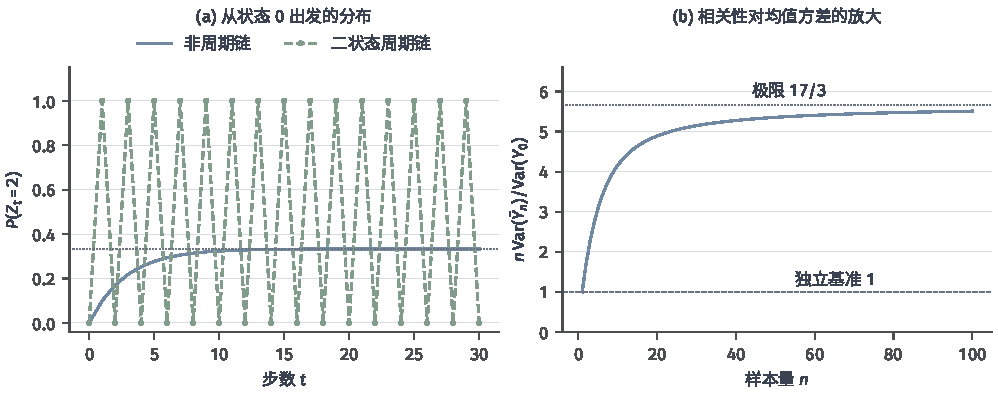
\includegraphics[width=\linewidth]{figures/02-mathematical-preliminaries-lower/01-random-variables-distributions-and-causality/matplotlib/stochastic-mixing-variance/figure.pdf}
  \caption{两状态链的解析式教学图。左图蓝线使用例~\ref{ex:stoch-two-state-chain}的转移矩阵，从\(Z_0=0\)出发绘制\(\mathbb P(Z_t=2)=(1-0.7^t)/3\)；绿线使用确定交替的转移矩阵。右图使用平稳初态和\(\rho_k=0.7^k\)，绘制\(1+2\sum_{k=1}^{n-1}(1-k/n)\rho_k\)，其极限为\(17/3\)，独立观测基准为\(1\)。}
  \label{fig:stochastic-mixing-variance}
\end{figure*}

\subsection{随机路径的收敛}
\label{sec:rv-path-convergence}
前面讨论同一个过程是否有连续版本；现在比较的是一列过程及其极限。路径极限
把整条函数当成随机对象，必须先规定函数之间怎样接近。对实值连续路径，
\(C([0,T])\)取一致距离
\(\|x-y\|_\infty=\sup_{t\leq T}|x(t)-y(t)|\)，是Polish空间。
对右连续且有左极限的路径，使用\(D([0,T])\)及Skorokhod \(J_1\)拓扑：
若存在严格递增的连续双射\(\lambda_n:[0,T]\to[0,T]\)，使
\[
\|\lambda_n-\operatorname{id}\|_\infty\to0,\qquad
\|x_n\circ\lambda_n-x\|_\infty\to0,
\]
就有\(x_n\to x\)于该拓扑。它允许跳跃时刻略微错开，再对齐比较；相应拓扑可由完备可分度量刻画。若极限连续，\(J_1\)收敛等价于一致收敛。

图~\ref{fig:probability-skorokhod-jump-alignment}用只有一次跳跃的路径说明时间校正的作用。令\(x(t)=\mathbb I\{t\geq1/2\}\)、\(x_n(t)=\mathbb I\{t\geq\tau_n\}\)，其中\(\tau_n=1/2+0.1/n\)。在两次跳跃之间，一条路径已经取\(1\)，另一条仍取\(0\)，所以普通一致误差始终等于\(1\)。取连接\((0,0)\)、\((1/2,\tau_n)\)、\((1,1)\)的分段线性\(\lambda_n\)，它是区间上的严格递增连续双射，并把目标跳跃时刻送到\(x_n\)的跳跃时刻。于是\(t<1/2\)时\(\lambda_n(t)<\tau_n\)，\(t\geq1/2\)时\(\lambda_n(t)\geq\tau_n\)，逐点得到\(x_n\circ\lambda_n=x\)，从而
\[
 \|x_n-x\|_\infty=1,\qquad
 \|\lambda_n-\operatorname{id}\|_\infty=0.1/n\longrightarrow0,\qquad
 \|x_n\circ\lambda_n-x\|_\infty=0.
\]
这个例子正好满足\(J_1\)的两个条件，却不满足普通一致收敛；极限路径的跳跃使这两种比较方式产生区别。

\begin{figure*}[htbp]
  \centering
  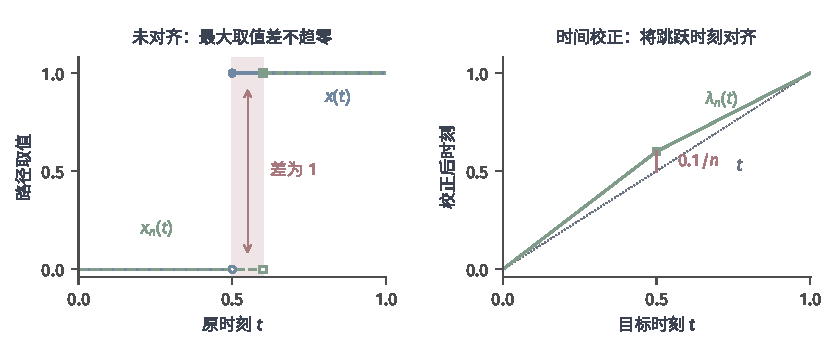
\includegraphics[width=140mm]{figures/02-mathematical-preliminaries-lower/01-random-variables-distributions-and-causality/matplotlib/probability-skorokhod-jump-alignment/figure.pdf}
  \caption{跳跃时刻对齐与\(J_1\)收敛（解析式教学图，展示\(n=1\)）。左图蓝实线的跳跃位于\(1/2\)，绿虚线的跳跃位于\(\tau_n=1/2+0.1/n\)；浅红时间带内二者取值相差\(1\)，实心与空心点区分端点是否取到。右图分段线性时间校正通过\((1/2,\tau_n)\)，相对恒等映射的最大偏差为\(0.1/n\)；经\(x_n\circ\lambda_n\)复合后，两条路径完全重合。}
  \label{fig:probability-skorokhod-jump-alignment}
\end{figure*}

有限维收敛仍不够。取确定连续函数
\[
x_n(t)=\max\{1-n^2|t-1/n|,0\},\qquad 0\leq t\leq1,\ n\geq2.
\]
每个固定时刻最终避开窄尖峰，所以任意有限维向量趋零；但
\(\|x_n\|_\infty=1\)，不可能在\(C([0,1])\)中趋零。
越来越窄的尖峰没有被有限个截面发现，却阻止了路径规律的紧性。

\begin{theorem}[连续路径的紧性与极限识别]
\label{thm:rv-continuous-path-tightness}
设\(X_n\)是\(C([0,T])\)值随机对象。令
\[
w(x,\delta)=\sup_{\substack{s,t\in[0,T]\\|t-s|\leq\delta}}|x(t)-x(s)|.
\]
若\((X_n(0))\)的分布一致紧，且对每个\(\varepsilon>0\)，
\[
\lim_{\delta\downarrow0}\sup_n
\mathbb P\{w(X_n,\delta)>\varepsilon\}=0,
\]
则路径分布一致紧。若其有限维分布还收敛到某个连续过程\(X\)的有限维分布，则
\(X_n\Rightarrow X\)于\(C([0,T])\)。
\end{theorem}
这里用到Arzelà--Ascoli定理的确定性形式：紧区间上一族连续函数若统一有界且等度连续，其一致范数闭包就是紧集。等度连续指对每个误差阈值，都能选择同一个时间间隔，同时控制族内全部函数的短时变化；每个函数各自连续还不够。Arzelà--Ascoli定理的证明见实分析教材\scite{math-folland1999real}；概率路径紧性的论证接着把这些紧集用于控制路径分布。

为把概率条件对应到这两项要求，固定\(0<\epsilon<1\)。由初值一致紧选\(M<\infty\)，使
\(\sup_n\mathbb P(|X_n(0)|>M)\leq\epsilon/2\)。
再取\(\eta_k=2^{-k}\)，逐个选取递减的\(\delta_k\downarrow0\)，使
\[
 \sup_n\mathbb P\{w(X_n,\delta_k)>\eta_k\}
 \leq\epsilon\,2^{-k-1},\qquad k\geq1.
\]
联合界说明每条\(X_n\)以至少\(1-\epsilon\)的概率同时满足初值界和全部尺度的振荡界。
满足这些限制的确定性路径族等度连续；把\([0,T]\)分成有限个长度不超过\(\delta_1\)的小段，还得到统一幅度界
\(M+\lceil T/\delta_1\rceil\eta_1\)。
因此其闭包是承载至少\(1-\epsilon\)概率的紧集，得到所需路径分布的一致紧性。

Prokhorov定理给出子列极限，坐标评价在\(C\)中连续，因此有限维规律识别每个子列极限。连续路径的Borel规律由稠密时刻坐标决定，故所有子列指向同一个极限。
若存在\(p>0\)、\(\beta>0\)及有限常数\(C\)，对全部\(n,s,t\)统一满足矩界
\(\mathbb E|X_n(t)-X_n(s)|^p\leq C|t-s|^{1+\beta}\)，且初值一致紧，则是上述模连续性条件的一项常用充分条件。

跳跃路径不能使用同一个连续模量：一个合法跳跃已使其无法趋零。对
\(D\)空间须另证\(J_1\)紧性，再在极限几乎必然连续的时刻核对有限维收敛。例如可用有界时间内的紧包含条件及停时短增量条件建立紧性；这些是额外假设，不由单时刻收敛自动成立。

缩放随机游走给出重要入口。若\(\xi_i\)独立同分布、均值零、方差一，
令\(S_k=\sum_{i=1}^k\xi_i\)，在网格\(k/n\)上取\(S_k/\sqrt n\)并作线性插值。
Donsker定理说明这些随机折线在\(C([0,T])\)中弱收敛到标准Brownian运动\scite{math-kallenberg2021probability}。
阶梯插值相应在\(D\)的\(J_1\)拓扑收敛。这里同时需要有限维极限与路径紧性，不能只把单时刻中心极限定理改写成带\(t\)的公式；Brownian的完整定义见第~\ref{sec:dynamical-brownian-motion}节，随机折线的构造则说明该路径规律怎样作为离散累计量的极限出现。


\section{本章小结}
\label{sec:stochastic-processes-and-approximation-summary}
\label{sec:random-sequences-and-processes-summary}

相同的单时刻分布可以对应不同的序列和路径。有限维联合规律保留坐标之间的联系，历史条件说明下一步允许依赖什么，路径条件则约束一次实现的连续性与跳跃。独立性、交换性、Markov性、鞅关系与平稳性各自限制不同的对象，不能由其中一种条件替代其余条件。

累计误差需要同时说明观测预算与结论的概率含义。固定时刻的集中不能自动覆盖看过记录后选出的时刻或候选；大数定律和中心极限定理也不直接给出当前预算下的误差概率。相关状态的时间平均可能收敛，而每一步的边缘规律仍周期振荡；路径极限又要求控制整族短时变化，超出逐个时刻极限所能保证的范围。

采样积分把这些结论用于给定规律下的计算。换测度保证平均目标可以改写，方差缩减还需额外的矩、辅助均值或条件积分信息；权重可计算与方差有限也须分别核对。随机比值和非线性变换的长期误差依赖概率阶、连续映射及局部展开，方差近似稳定并不免除反变换偏差。下一章将把给定规律改为未知观测模型，研究有限记录能够支持哪些统计结论。
